% !Mode:: "TeX:UTF-8"
%!TEX program  = xelatex

%\documentclass[bwprint,fontset=windows]{gmcmthesis}
\documentclass[bwprint]{gmcmthesis}

\hypersetup{hidelinks}
\usepackage[framemethod=TikZ]{mdframed}

%\usepackage{fontspec}  % for Consolas & Courier New
%\lstset{basicstyle=\small\fontspec{Consolas}}
%\lstset{basicstyle=\small\fontspec{Courier New}}
%\setmonofont{Consolas}
%\setcounter{tocdepth}{3}   % 调整目录深度

\usepackage{subfig}
\usepackage{colortbl}
\usepackage{makecell}
\usepackage{xcolor}
\definecolor{color1}{rgb}{0.78,0.88,0.99}
\definecolor{color2}{rgb}{0.36,0.62,0.84}
%\definecolor{color3}{rgb}{0.8235,0.8706,0.9373}
\definecolor{color3}{rgb}{0.88,0.92,0.96}
\definecolor{color4}{rgb}{0.96,0.97,0.98}%{0.9176,0.9373,0.9686}

% 算法
\usepackage[noend]{algpseudocode}
\usepackage{algorithmicx,algorithm}
\floatname{algorithm}{算法}
\renewcommand{\algorithmicrequire}{\textbf{输入:}}
\renewcommand{\algorithmicensure}{\textbf{输出:}}

%\numberwithin{equation}{section}
%\numberwithin{figure}{section}
%\numberwithin{table}{section}


\newcommand{\red}[1]{\textcolor{red}{#1}}
\newcommand{\blue}[1]{\textcolor{blue}{#1}}


%===================== 建模论文题目 ======================

\title{针对出血性脑卒中临床智能诊疗的建模}
\baominghao{\hspace{6em} 23101460004} %参赛队号
\schoolname{\hspace{5.8em} 辽宁科技大学} %学校名称
\membera{\hspace{6em} 谭旭} %队员A
\memberb{\hspace{6em} 肖俊} %队员B
\memberc{\hspace{6em} 蒋浩彦} %队员C

%=======================================================


\begin{document}

	%生成标题
	\maketitle
	
	%填写摘要
	\begin{abstract}
		脑卒中(中风)是一种急性脑血管疾病,可以分为缺血性、出血性和短暂性脑缺血。中国脑卒中患病率自1990年以来增加了147.5\%,这说明该问题亟需加强研究和检测。各种危险因素如高血压、吸烟、糖尿病等都会导致脑卒中风险增加。因此,对出血性脑卒中的智能化临床诊疗是有着长远意义,是非常值得研究的方向。
		
		\textbf{针对问题一}:我们充分进行数据分析与处理,进一步对限制要求进行分情况判断后,发现存在难判断的超过48h也超过阈值的多个对象,我们通过建立短期线性预测模型,考虑患者血肿变化率,拟合出了患者48小时内是否发生血肿扩张的具体时间情况。对于所有患者的血肿扩张概率预测我们则是采用了一种\textbf{基于Channel Attention注意力机制的集成学习加权模型},我们在其中加入了支持向量机SVM、多层感知机MLP、随机森林、LightGBM以及XGBoost进行基于通道注意力的加权计算,得到综合多模型输出的全体患者血肿扩张概率预测结果,该结果达到\textbf{81\%正确率},相比单一模型\textbf{提升近10个点},结果表明我们的方法比单一模型或普通集成模型具有更好的效果以及更好的泛化性和健壮性。
		
		\textbf{针对问题二}:我们将数据进行了对特征的转换,以及通过自定义的水肿变化率提炼算法对多个特征进行共同表达,完成了特征生成凝练工作,随后我们在得到的数据上使用多种函数拟合方式,包括\textbf{线性拟合、二次多项式拟合、高斯拟合和四次多项式拟合},通过对比四种结果拟合曲线,我们发现使用四次多项式函数可以相对较好的拟合全体患者水肿体积随时间进展曲线,其平均残差仅为\textbf{1.2626}。对于人群亚组的分类,我们则采取\textbf{K-means聚类},将人群分为了三组,分别对应:易水肿人群、普通人群、水肿抵抗人群。对于众多因素相关性的分析,我们则采取了\textbf{斯皮尔曼系数、肯德尔系数、灰色关联度系数以及随机森林}进行平均相关性分析,同时采用单因素与多因素方差分析和热力图等辅佐我们对关系做出判断。
		
		
		\textbf{针对问题三}:我们同样采用问题一的集成学习方式进行建模,通过对\textbf{LightGBM、XGBoost、随机森林、MLP以及KNN聚类进行集成投票},我们获得了患者90天mRS的投票预测结果,同时,为了使效果能够逼近问题一的加权模型,我们对投票模型进行了参数搜索,采用\textbf{多次迭代网格搜索},并采用更合理的交叉验证,我们将原来投票模型的性能提升了\textbf{10\%},模型的泛化性得到可观的提高。最后,我们通过采用随机森林重要性排序等方法获得了多因素之间的关联关系,我们提出了一系列针对血肿水肿检测预防处理措施、对糖尿病以及高龄高血压病患者给出了预后相关建议。
	
	
		\keywords{脑卒中智能诊疗\quad 数据挖掘\quad \textbf{集成学习}\quad\textbf{相关性分析}\quad\textbf{注意力机制}}
	
	\end{abstract}
	
	\pagestyle{plain}
	
	%目录 不推荐加
	\maketoc
	
	\clearpage
	
	\section{问题重述}
		\subsection{问题背景}   % 问题的背景
		
			脑卒中(cerebral stroke)国内习惯称为“中风”,是一种急性脑血管疾病,是由于脑部血管突然破裂或因血管阻塞导致血液不能流入大脑而引起脑组织损伤的一组疾病。通常脑卒中表现为缺血性脑卒中、出血性脑卒中以及短暂性脑缺血(TIA)。据文章\cite{ma2021temporal}统计,1990年至2019年,中国的脑卒中患病人数从1990年的2880万例增加了147.5\%。在不同类型的脑卒中中,缺血性脑卒中的患病率增加最多,增长超195.2\%,其次是蛛网膜下腔出血(54.8\%)和脑出血(43.0\%)。
			
			虽然出血性脑卒中在脑卒中的病例组成中占比相对较少,但基于我国庞大的人口基数,出血性脑卒中的研究和检测任然是亟待解决的问题。现代引发脑卒中的因素逐渐增多,高血压、吸烟、糖尿病、高胆固醇、肥胖、心血管疾病等等,很多危险因素在不同地区和人群中造成了不同程度的健康问题,研究表明\cite{feigin2014global},1990年至2010年期间,在高收入国家中,出血性中风的发病率显著降低了19\% ,死亡率降低了 38\%,相比之下,中低收入国家出血性中风的发病率显著增加了22\%,这说明发达国家与发展中国家在病情的预防、检测、治疗中任然存在很大差距。
			
			因此,我国加强对出血性脑卒中的临床诊疗智能化,成为了为患者解决检测治疗难点的重要环节之一,成为了近些年来该领域的热点问题。根据中华医学会神经病学分会在中华神经科杂志中发表的《中国脑出血诊治指南(2019)》\cite{strock2019bib}中所指导的诊治流程,诊治脑卒中通常流程为:院前处理、诊断与评估(病史与体征、影像学检查、实验室检查、疾病诊断)、脑出血治疗(内科治疗、外科治疗),如图\ref{fig:1}所示。
			
			在确定出血性脑卒中后,后续血肿范围的扩大是一个不利预后的重要风险因素之一。在出血发生后的短时间内,由于多种原因,如脑组织受损和炎症反应,血肿范围可能逐渐增大,导致颅内压急剧上升,从而加剧神经功能受损,甚至危及患者的生命。因此,监测和控制血肿的扩张是医疗关注的一个要点。此外,血肿周围的水肿作为脑出血后继发性损害的标志已引起广泛临床关注。血肿周围的水肿可能导致脑组织受到挤压,进而影响神经元的功能,使脑组织受损程度进一步加重,从而恶化患者的神经功能。综上所述,早期识别和预测出血性脑卒中后血肿扩张和血肿周围水肿的发生和发展对于改善患者的预后和提高其生活质量具有重要意义。
			
			\begin{figure}[H]
				\centering
				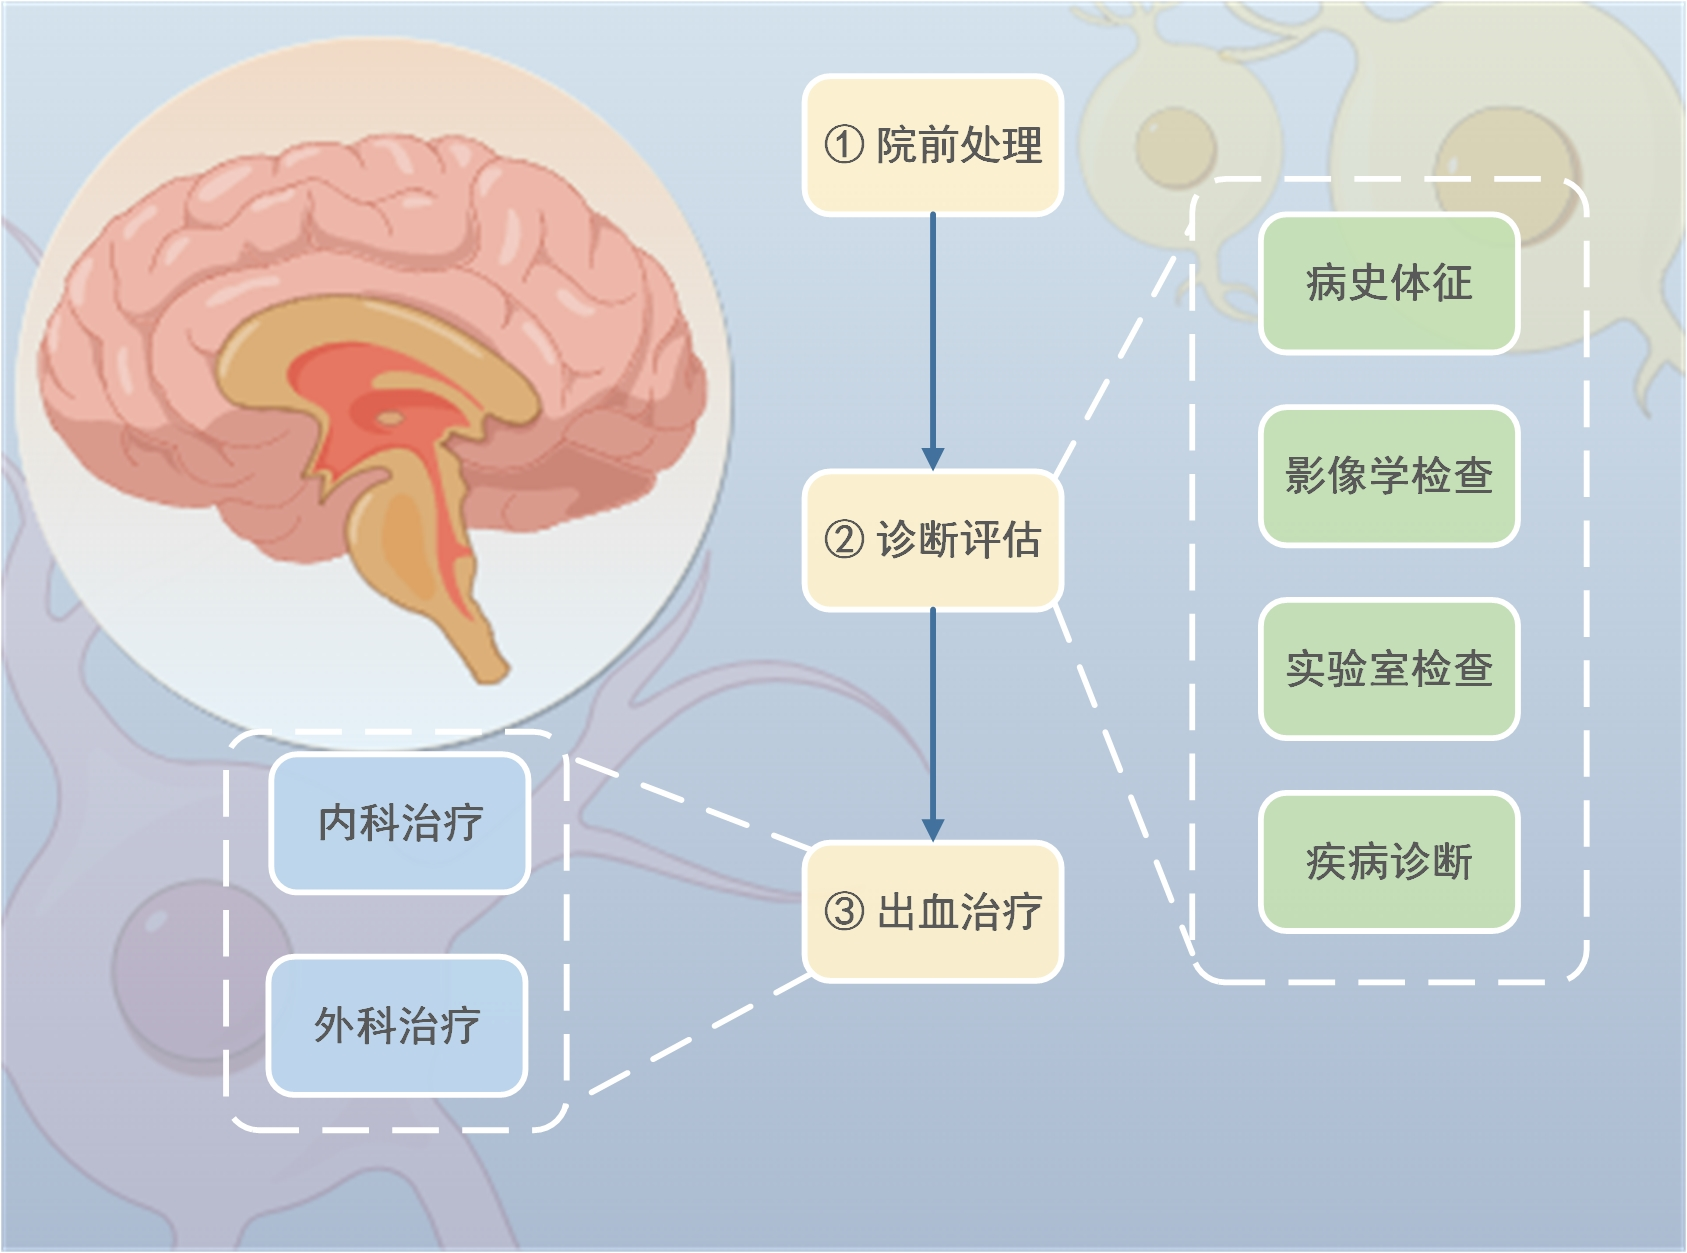
\includegraphics[width=.80\textwidth]{诊断流程图.jpg}
				\caption{诊断流程图}
				\label{fig:1}
			\end{figure}
		
		
		\subsection{问题的提出}
		
		%\subsubsection{问题的提出内容一}
		
			针对上述问题背景的研究,本文需要依次研究解决如下问题:
			
			\textbf{问题一(血肿扩张风险因素探索):} 首先,根据入院首次影像检查流水号、发病到首次影像检查时间间隔、各时间点流水号及对应的HM\_volume,判断患者sub001至sub100发病后48小时内是否发生血肿扩张事件,并同时记录血肿扩张发生时间。是否发生血肿扩张按照规则:后续检查比首次检查绝对体积增加≥6mL或相对体积增加≥33\%。结果填写规范为:1(发生血肿扩张)、0(未发生血肿扩张);时间保留两位小数,如10.33小时。
			
			其次,基于前100例患者个人史、疾病史、发病及治疗相关特征、影像检查结果(首次),以及获取到的是否发生血肿扩张情况,构建训练数据,要求预测所有患者(sub001至sub160)发生血肿扩张的概率。结果填写规范为:记录预测事件发生概率(取值范围0-1,小数点后保留4位数)。答案填写完整形式如表\ref{tab:ans1}所示:
			
			\begin{table}[H]
				\caption{问题一答案样式}
				\label{tab:ans1}
				\rowcolors{2}{gray!10}{white}
				\resizebox{\textwidth}{!}{
					\begin{tabular}{ccc}
						\toprule[1.5pt]
						\makebox[0.3\textwidth][c]{是否发生血肿扩张} & \makebox[0.3\textwidth][c]{血肿扩张时间(单位:小时)} &
						\makebox[0.4\textwidth][c]{血肿扩张预测概率}\\
						\midrule[1pt]
						1 & 10.33 & 0.8143\\
						\bottomrule[1.5pt]
					\end{tabular}	
				}		
			\end{table}
			
			
			\textbf{问题二(血肿周围水肿进展和治疗关联探索):}首先,根据前100个患者(sub001至sub100)的水肿体积(ED\_volume)和重复检查时间点,构建一条全体患者水肿体积随时间进展曲线$y=f(x)$,要求x轴为发病至影像检查时间,y轴为水肿体积。并记录真实值与拟合曲线之间存在的残差。
			
			其次,探索患者水肿体积随时间进展模式的个体差异,构建不同人群(分亚组:3-5个)的水肿体积随时间进展曲线,同样记录前100名患者真实值与曲线间的残差。
			
			最后,分析不同治疗方法对水肿体积进展模式的影响,以及分析血肿体积、水肿体积、及治疗方法三者之间的关系。同样,该题需要记录答案,答案完整形式如表\ref{tab:ans2}所示:
			
			\begin{table}[H]
				\caption{问题二答案样式}
				\label{tab:ans2}
				\rowcolors{2}{gray!10}{white}
				\resizebox{\textwidth}{!}{
					\begin{tabular}{ccc}
						\toprule[1.5pt]
						\makebox[0.3\textwidth][c]{残差(全体)} & \makebox[0.3\textwidth][c]{残差(亚组)} &
						\makebox[0.4\textwidth][c]{所属亚组(取值范围:0、1、2)}\\
						\midrule[1pt]
						8.3416 & 2.3157 & 1\\
						\bottomrule[1.5pt]
					\end{tabular}	
				}		
			\end{table}
			
			
			\textbf{问题三(患者预后预测及关键因素探索):}首先,要求根据前100个患者(sub001至sub100)个人史、疾病史、发病相关、首次影像结果构建预测模型,预测患者(sub001至sub160)90天mRS评分。
			
			其次,根据前100个患者(sub001至sub100)所有已知临床、治疗、影像(首次+随访)检测结果,以及前面所得的患者90天mRS评分情况构建训练集,来预测所有含随访影像检查的患者(sub001至sub100,sub131至sub160)90天mRS评分。所有的mRS评分预测结果填写格式为0-6的有序等级变量。
			
			最后,通过分析患者预后90天mRS、个人史、疾病史、治疗方法及影像特征等等的关联关系,提出临床相关决策提出建议。
			
			
			为方便后文建模理解,对问题给定数据和附件的解读如表\ref{tab:datasets}所示:
			
			\begin{table}[H]
				\caption{给定附件解释}
				\label{tab:datasets}
				\rowcolors{2}{gray!10}{white}
				\resizebox{\textwidth}{!}{
					\begin{tabular}{cl}
						\toprule[1.5pt]
						\makebox[0.4\textwidth][c]{附件名} & \makebox[0.5\textwidth][c]{内容解释} \\
						\midrule[1pt]
						表1:患者列表及临床信息 & 记录mRS、患者信息、病史、发病相关特征及治疗相关特征\\
						表2:患者影像信息血肿及水肿的体积及位置 & 记录患者多次检查血肿和水肿影像信息(体积与位置)\\
						表3:患者影像信息血肿及水肿的形状及灰度分布 & 记录患者多次检查血肿和水肿影像信息(形状和灰度分布)\\
						表4:答案文件 & 针对三个问题的结果汇总填写 \\
						附件1:检索表格-流水号vs时间 & 记录患者检测次数及每次的对应时间 \\
						
						\bottomrule[1.5pt]
					\end{tabular}	
				}		
			\end{table}
		

	\section{模型的假设}
		本次模型构建过程中,通过充分了解问题栈的深度和广度,为了方便后续简化赛题、排除其他因素的干扰,我们提出以下几点假设:\par
		(1)假设赛题提供的160例患者数据真实有效,不存在明显分布偏差。\par
		(2)假设\textbf{不同患者个人数据相同、流水号不匹配等异常数据}是人因因素导致,后续处理过程中进行处理后,数据分布与真实情况误差在可接受范围内。\par
		(3)假设血肿、水肿影像特征数据中,按不同部位划分的检测数据能够表示大脑情况的总体变化,存在正确的正相关或负相关性。\par
		(4)假设患者大脑血肿、水肿体积随时间变化不会发生剧烈震荡变化,血肿和水肿不会出现异常突变。\par
	
	
	
	\section{符号说明}
	
		本文所用到的关键符号及其符号意义如表\ref{tab:means}所示: 
		
		\begin{table}[H]
			\caption{符号说明}
			\label{tab:means}
			\rowcolors{2}{gray!10}{white}
			\begin{tabular}{cc}
				\toprule[1.5pt]
				\makebox[0.4\textwidth][c]{符号} & \makebox[0.5\textwidth][c]{符号意义} \\
				\midrule[1pt]
				mRS & 评估脑卒中患者功能状态和残疾程度,范围0到6\\
				Hemo & 血肿\\
				ED & 水肿\\
				Accuracy & 准确率 \\
				Precision & 精确率\\
				Recall & 召回率\\
				AUC & 曲线下面积 \\
				F1-Score & Precision和Recall的加权调和平均 \\
				\bottomrule[1.5pt]
			\end{tabular}			
		\end{table}
	
	
	\section{问题的分析}
		\subsection{【问题一】血肿扩张风险相关因素探索建模}
			\subsubsection{问题分析1a:48小时内血肿扩张判断}\label{sec:4.1.1}
				如果想要判断患者sub001至sub100发病后48小时内是否发生血肿扩张,并记录血肿扩张发生时间,我们需要获取到患者发病到首次检查前的时间间隔$\alpha$,以及第i次随访检查与上一次随访检查之间的间隔$\beta_i$,来作为48小时时间约束条件的判断,按照公式\ref{eq:1}计算每个患者发病后所隔时间,其中n为不超过48小时内的检测次数:
				\begin{equation}
					\label{eq:1}
					T=\alpha+\sum_{i=i}^{n}\beta_{i}
				\end{equation}
				
				同时,作为血肿扩张的重要判断依据,我们同样需要拿到患者首次检测的血肿体积$V_1$,以及第i次检测的血肿体积$V_i$,通过计算血肿体积前后变化,按照判断依据,定性的判断血肿扩张程度是否超过设定阈值,判断依据如公式\ref{eq:2}所示,0表示未超过血肿扩张阈值,1表示超过血肿扩张阈值:
				\begin{equation}
					\label{eq:2}
					\begin{cases}0,\quad V_{\mathrm{i}}-V_{1}<6\quad or\quad \frac{V_{i}-V_{1}}{V_{i}}\times100\%<33\%\\1,\quad V_{\mathrm{i}}-V_{1}\ge 6\quad or\quad \frac{V_{i}-V_{1}}{V_{i}}\times100\%\ge 33\%&\end{cases}
				\end{equation}
				
				通过实际对数据集进行观察,我们发现此题难点在于以下几处:
				
				\textbf{难点1:}数据表1与数据表2中,虽不存在缺失值,但160个患者信息里存在个别异常值,还有数据表与其他数据表匹配异常的问题。因为最终需要预测的答案里有异常对象,所以需要妥善处理异常值。
				
				\textbf{难点2:}实际按照时间和血肿扩张两个约束条件做患者判断时,情况会非常复杂,按照排列组合会出现四种情况,针对每种情况都需要做单独分析。
				
				\textbf{难点3:}血肿扩张发生时间难以精确推断,与患者何时进行发生血肿扩张前的最后一次检测时间以及两次检测时间的间隔有关。我们需要去用某种方式判断可能的相对精确血肿扩张发生时间。
				
				针对上述三个难点,我们建立了解决该问题的完整解题流程,对于三个难点的解答如下:
				
				对于难点1,我们发现患者sub003与sub131、患者sub004与sub132的患者临床信息一致,我们认为这是在数据采样环节出现了完全随机异常,可以假设为人因因素导致,正常情况下,我们会采取将后两者视作出现问题的异常值剔除,但是后续赛题频繁涉及对所有患者进行某种预测或分析,所以剔除两位患者并不合理,且数据样本量仅有160,赛题本身属于少样本学习,故每一条样本数据都弥足珍贵,所以我们采取了异常值处理中的忽略策略,不对异常患者进行处理。对于sub74患者流水号信息在两表之间不一致的情况,我们通过观察多表流水号数据,发现仅有一表与其他表不同,是可以人为修正的异常,故采取直接修改数据的方式进行异常值处理。
				
				对于难点2,当我们进一步进行分析会发现,每次循环判断约束条件时所划分出来的四种情况对应的含义如图\ref{fig:3}所示。
				
				\begin{figure}[H]
					\centering
					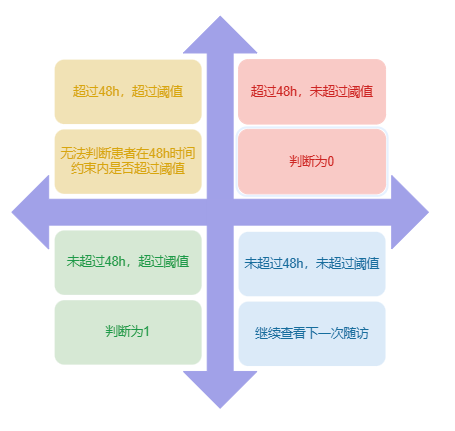
\includegraphics[width=.65\textwidth]{四种情况具体含义.png}
					\caption{四种情况具体含义}
					\label{fig:3}
				\end{figure}
				
				对每一个患者循环进行计算判断时,最终都会落入到一、二、三象限中得到收敛结果。象限一表示后续随访检测已经超过48h,此时仍然未超过阈值,基于血肿体积不会剧烈迅速变化的假设,我们可以认为该患者48h内未发生血肿扩张;象限三表示后续随访检测没有超过48h,而这时已经超过了体积变化阈值,我们可以认为该患者48h内发生了血肿扩张情况;象限四表示后续随访检测即没有超过48h,也没有超过血肿变化阈值,我们应该继续看该患者的下一次随访情况,再做一次四象限判断;最后,象限二表示后续随访检测已经超过了48h,而此时也出现了血肿扩张超过阈值,这种情况我们无法判断血肿扩张情况是在48h内发生的,还是48h外发生的,需要做特别处理。以上情况判断的算法如下所示:
				
				\begin{center}
					\begin{minipage}{0.8\textwidth}
						\begin{algorithm}[H]%[!htp]
							\caption{血肿扩张情况判断} %算法的名字
							{\bf 输入:} %算法的输入, \hspace*{0.02in}用来控制位置,同时利用 \\ 进行换行
							已处理过后的患者临床信息与血肿信息内联表\\
							{\bf 输出:} %算法的结果输出
							各个患者血肿扩张情况(0,1,-255)
							\begin{algorithmic}[1]
								\State Stroke Estimate
								\For{sub\_num} % For 语句,需要和EndFor对应
								\State time = seg\_time 
								\State volume = volume\_change
								\If{time > 48 and volume < 6} % If 语句,需要和EndIf对应
								\State \Return 0
								\EndIf
								\If{time < 48 and volume > 6} % If 语句,需要和EndIf对应
								\State \Return 1
								\EndIf
								\If{time > 48 and volume > 6} % If 语句,需要和EndIf对应
								\State \Return -255
								\EndIf
								\If{time < 48 and volume < 6} % If 语句,需要和EndIf对应
								\State \textbf{continue}
								\EndIf
								\EndFor
							\end{algorithmic}
						\end{algorithm}
					\end{minipage}
				\end{center}
				
				而对于难点3的异常情况,我们认为仅通过凭感觉猜测其血肿扩张是否发生在48h以内,或者统一设置为某个值是不合理的,由于通过检查患者血肿体积随时间变化的趋势情况,我们发现患者血肿体积随时间短期内基本表现为线性,部分患者拟合的趋势曲线如图\ref{fig:four pic}所示:
				
				
				\begin{figure}[H]
					\centering
					\subfloat[sub001]{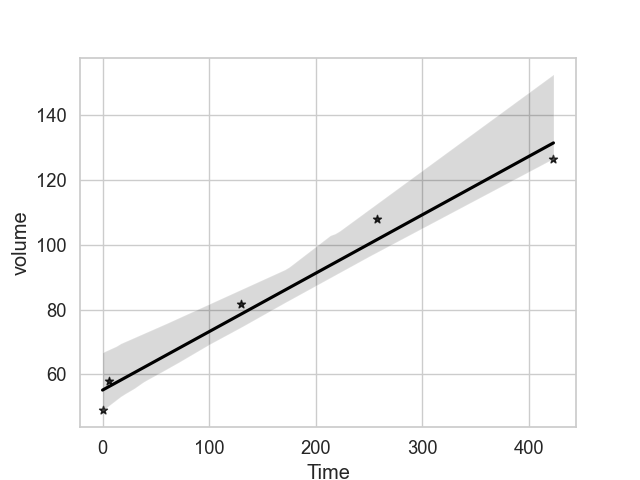
\includegraphics[width=0.28\textwidth]{sub1_self.png}}\qquad
					\subfloat[sub007]{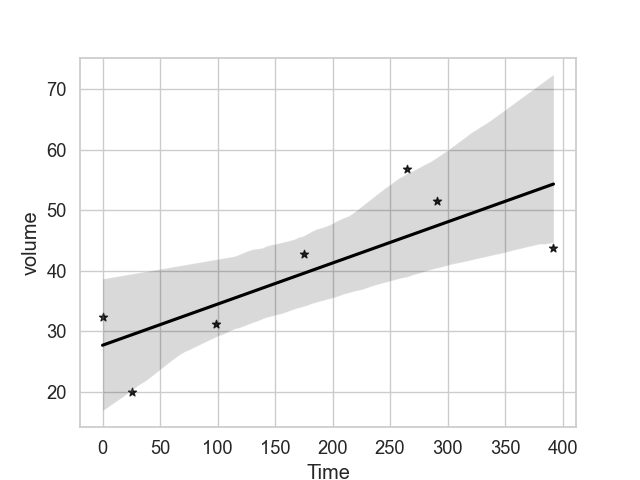
\includegraphics[width=0.28\textwidth]{sub7_self.png}} \\
					\subfloat[sub023]{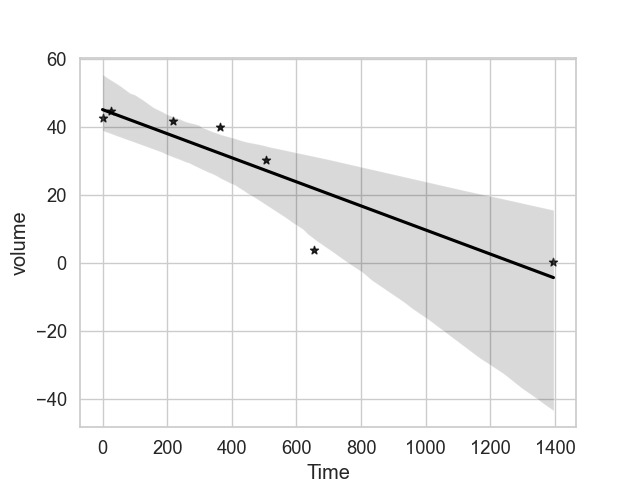
\includegraphics[width=0.28\textwidth]{sub23_self.png}}\qquad
					\subfloat[sub064]{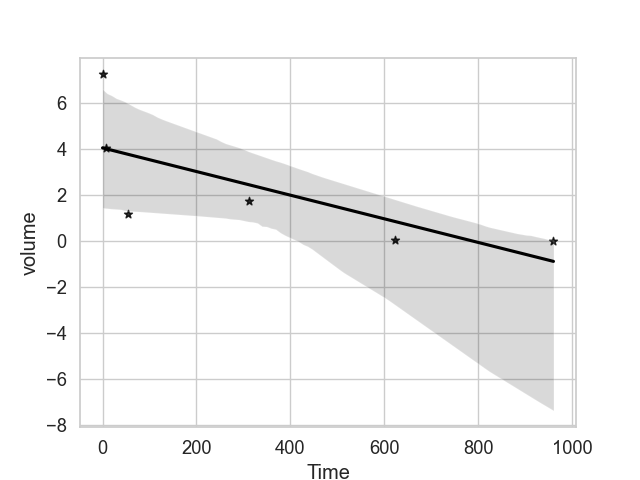
\includegraphics[width=0.28\textwidth]{sub64_self.png}}
					\caption{部分患者血肿体积随时间变化情况}
					\label{fig:four pic}
				\end{figure}
				
				因此我们选择对每一个难判断的患者计算其血肿扩张变化率$V_i$,然后通过查询发病到首次检查间隔时间$\alpha_i$,按照公式$\tau=\frac{6}{V_i}$定量预测患者若出现血肿扩张现象所需时间$\tau$,从而依据$\alpha_i+\tau$与48h对比,判断是否出现血肿扩张情况,并将其作为患者发生水肿的时间。
				
				
				
				
			\subsubsection{问题分析1b:所有患者血肿扩张概览预测}
				问题意图通过从表1、表2、表3中前100例患者的个人史、疾病史、发病与治疗相关特征、以及多个影像检查结果与是否发生血肿扩张事件的关系中去建立模型,使该模型能够很好的预测所有患者是否发生血肿扩张的概率。
				
				本题的目标变量为上一小问中获取到的前100例患者血肿扩张情况,由于要求的限制,只能纳入患者首次影像检查的结果作为数据输入,所以我们先要将符合要求的自变量和因变量重新构建一个适合该题训练的新数据集,同时,我们留意到新数据集的构建过程中,特征的维度将变大,各特征之间也存在一定的相关性,如表3中多个灰度特征与形状特征,在描述一个趋势的时候表达相同或相近的含义,一定程度上造成了冗余,所以构建新数据集后的数据处理也非常重要。
				
				我们要预测的结果为患者是否发生血肿扩张的概率,该概率为0到1之间的一个值,越接近0则表示没有发生,反之则表示发生血肿扩张,通常在机器学习中我们采用建立分类预测模型的方式来解决此类问题。
				
				常见的分类预测模型大体上分为机器学习类与神经网络类,通过探索赛题数据量以及对数据类型的初步观察,我们认为机器学习非常适合本题数据样本量较少的预测情况。通过学习和查找相关资料,我们选择了一种融合LightGBM、MLP、RF、XGB、SVC模型的基于注意力机制的类集成学习模型——\textbf{Channel Attention加权集成学习模型},通过训练模型并按照注意力得分加权各算法结果,最终可以获得我们需要的预测结果。
				
				问题一整体系统流程图如下所示:
				
				\begin{figure}[H]
					\centering
					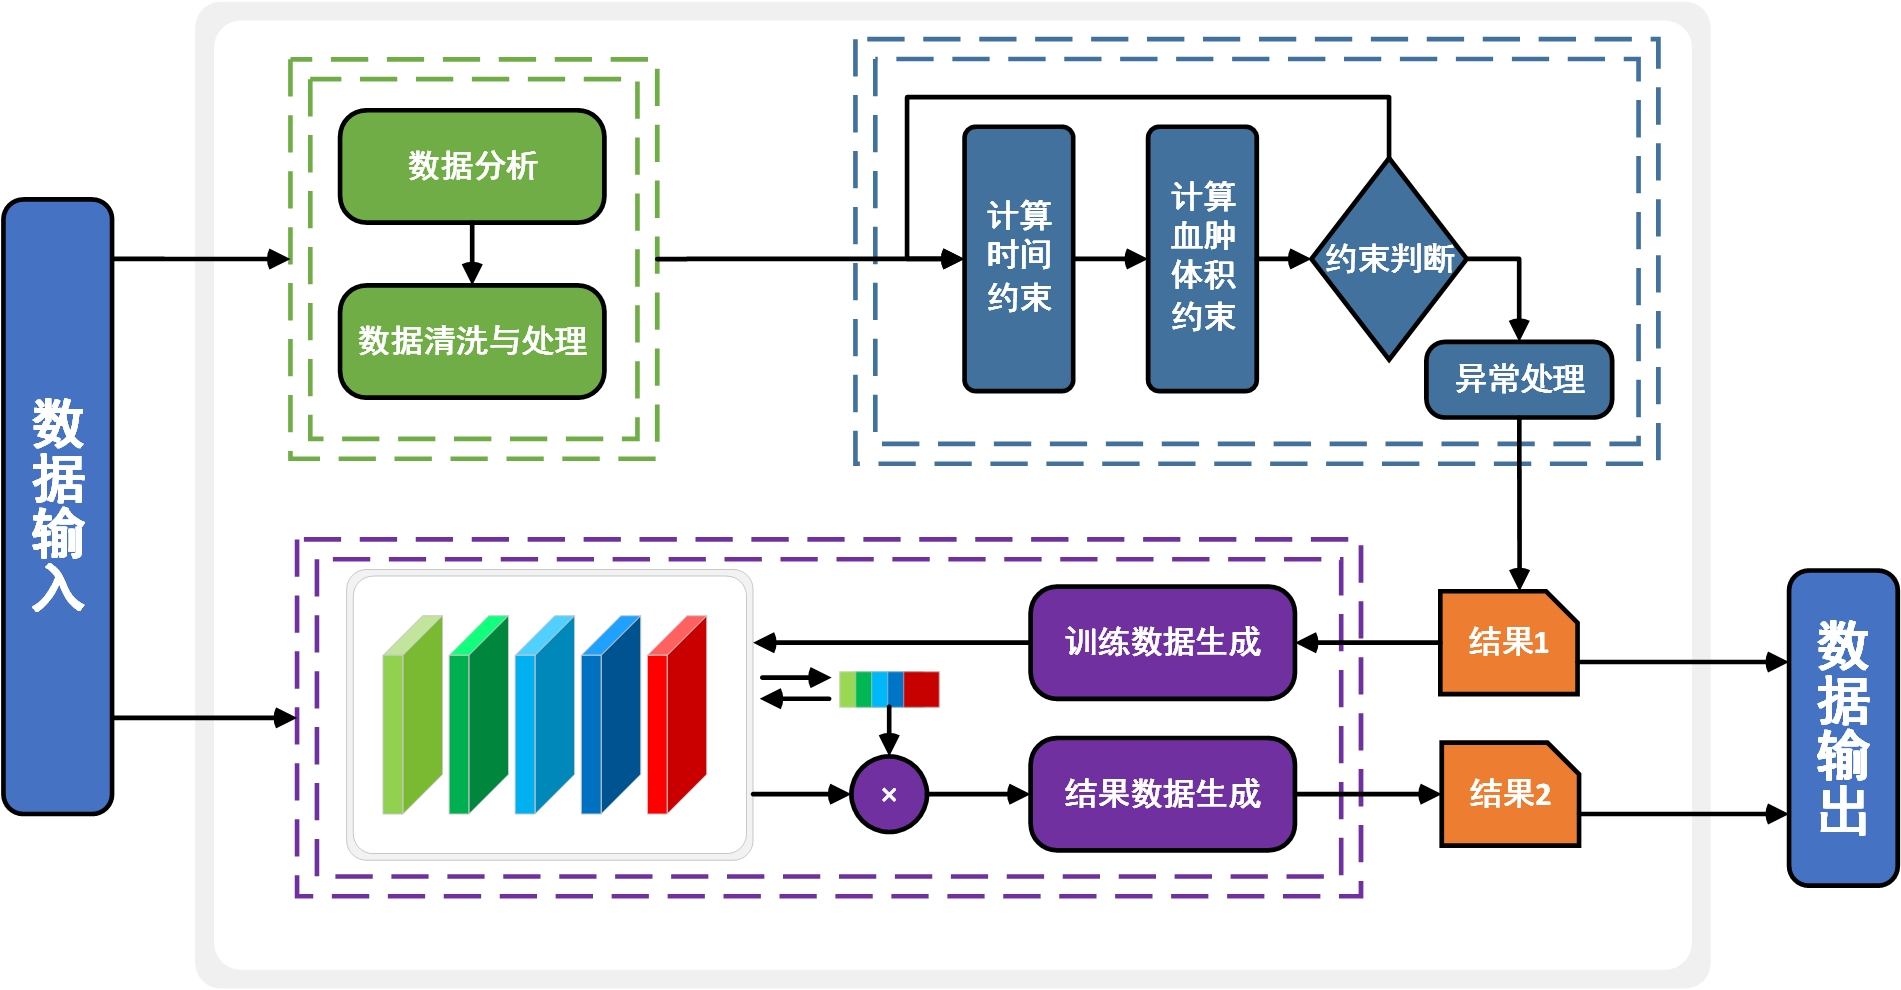
\includegraphics[width=.82\textwidth]{问题1系统图.jpg}
					\caption{问题一系统图}
					\label{fig:4}
				\end{figure}
				
			\subsubsection{理论基础}\label{lilun}
				\textbf{一、支持向量机SVM} 
				
				\textbf{1. 简介}
				
				支持向量机(support vector machines, SVM)是一种二分类模型,它的基本模型是定义在特征空间上的间隔最大的线性分类器,间隔最大使它有别于感知机;SVM还包括核技巧,这使它成为实质上的非线性分类器。SVM的的学习策略就是间隔最大化,可形式化为一个求解凸二次规划的问题,也等价于正则化的合页损失函数的最小化问题。SVM的的学习算法就是求解凸二次规划的最优化算法。在Python的Sklearn库中,SVM被实现为SVR和SVC两种类,SVR负责计算回归问题,SVC负责计算分类问题。
				
				\textbf{2. 原理}
				
				\textbf{【最大间隔平面】}
				
				支持向量机的目标是找到一个超平面,使得两个类别之间的间隔最大化。这个间隔被称为“间隔”,它是两个类别中距离超平面最近的数据点到超平面的距离之和。假设超平面的方程为:
				\begin{equation}
					w\cdot x+b=0 \nonumber
				\end{equation}
				
				其中, $w$是法向量, $b$是截距, $x$是输入特征。我们希望找到$w$和$b$,使得间隔最大化。
				
				\textbf{【支持向量】}
				
				支持向量是距离超平面最近的数据点,它们决定了超平面的位置。支持向量满足以下条件:
				\begin{equation}
					y_i(w\cdot x_i+b)=1 \nonumber
				\end{equation}
				
				其中, y\_i 是数据点 x\_i 的类别标签,取值为1或-1。
				
				\textbf{【核函数】}
				
				支持向量机的一个重要扩展是核技巧(Kernel Trick),它允许我们在高维空间中进行分类。核函数可以将数据从低维空间映射到高维空间,从而实现非线性分类。
				
				常见的核函数包括线性核、多项式核、高斯径向基核(RBF)等。
				
				\textbf{二、XGBoost梯度提升}
				
				\textbf{1. 简介}
				
				XGBoost(eXtreme Gradient Boosting)极致梯度提升,是一种基于GBDT的算法或者说工程实现。XGBoost的基本思想和GBDT相同,但是做了一些优化,比如二阶导数使损失函数更精准;正则项避免树过拟合;Block存储可以并行计算等。XGBoost具有高效、灵活和轻便的特点,在数据挖掘、推荐系统等领域得到广泛的应用。XGBoost特别适用于分类和回归问题,在性能和效率上取得了巨大的改进。
				
				\textbf{2. 原理}
				
				XGBoost的核心原理是通过迭代训练一系列决策树模型,然后将它们组合成一个强大的集成模型。每个决策树都是弱学习器,它们通过对之前模型的残差进行拟合来逐步改进预测结果。以下是XGBoost的核心原理步骤:
				
				\begin{table}[H]
					\centering
					\rowcolors{1}{gray!8}{white}
					\begin{tabularx}{\textwidth}{|X|}
						\hline
						\begin{enumerate}
							\item \textbf{初始化模型}:用一个简单的模型(通常是平均值)来预测目标变量。
							\item \textbf{计算残差}:计算当前模型对目标变量的预测误差,这被称为残差。
							\item \textbf{拟合决策树}:训练一个决策树模型来拟合残差,目标是最小化残差的损失函数(通常使用均方误差或对数损失)。
							\item \textbf{更新模型}:将新训练的决策树模型的输出与之前的模型相加,从而更新整体模型。
							\item \textbf{重复迭代}:重复步骤2至4,每次迭代都在之前模型的基础上进一步减小残差。
							\item \textbf{正则化}:为了控制模型的复杂度,XGBoost引入了正则化项,如L1和L2正则化,以防止过拟合。
							\item \textbf{终止条件}:迭代可以根据某个停止标准(如达到最大迭代次数或残差变化不大)而终止。
							\item \textbf{生成最终模型}:将所有决策树模型的输出相加,得到最终的预测结果。
						\end{enumerate}\\
						\hline
					\end{tabularx}
				\end{table}
				
				
				
				XGBoost的目标函数是一个关于模型的损失函数和正则化项的加权组合。具体地,XGBoost的目标函数可以表示为:
				\[
				\mathcal{L}(\theta) = \sum_{i=1}^{n} L(y_i, \hat{y}_i) + \sum_{k=1}^{K} \Omega(f_k)
				\]
				
				其中:
				
				\begin{table}[H]
					\centering
					\rowcolors{1}{gray!8}{white}
					\begin{tabularx}{\textwidth}{|X|}
					\hline
					\begin{itemize}
						\item $\mathcal{L}(\theta)$ 是目标函数。
						\item $n$ 是训练样本的数量。
						\item $L(y_i, \hat{y}_i)$ 是损失函数,用于衡量模型对第 $i$ 个样本的预测误差。
						\item $K$ 是树的数量。
						\item $f_k$ 是第 $k$ 个树。
						\item $\Omega(f_k)$ 是正则化项,用于控制树的复杂度。
					\end{itemize}\\
					\hline
				\end{tabularx}
				\end{table}
				
				XGBoost的目标是最小化目标函数 $\mathcal{L}(\theta)$ 关于模型参数 $\theta$ 的值。这通常通过梯度下降等优化算法来实现。
				
				\textbf{三、MLP多层感知机}
				
				\textbf{1. 简介}
				
				MLP(多层感知机)是一种常用于机器学习和深度学习任务的神经网络模型。它是一种前馈神经网络,由多个神经元组成的多层结构,具有输入层、隐藏层和输出层。MLP通过学习从输入数据到输出标签之间的映射关系来解决分类和回归问题。每个神经元都与前一层的所有神经元相连,通过权重和激活函数来传递信号。MLP是深度学习中的基础模型,通过增加隐藏层和神经元的数量,可以构建更复杂的神经网络架构来解决各种机器学习任务。
				
				\textbf{2. 原理}
				
				MLP的原理基于神经元的连接和激活。以下是MLP的核心原理:
				
				\begin{table}[H]
					\centering
					\rowcolors{1}{gray!8}{white}
					\begin{tabularx}{\textwidth}{|X|}
					\hline
					\begin{enumerate}
						\item \textbf{输入层}:输入层接受特征数据作为输入,每个特征对应一个输入神经元。
						\item \textbf{隐藏层}:隐藏层是位于输入层和输出层之间的一层或多层神经元。每个隐藏层神经元都连接到前一层的所有神经元,并具有权重。隐藏层的数量和每层的神经元数量是模型的超参数。
						\item \textbf{输出层}:输出层产生模型的最终输出,通常用于分类问题的分类标签或回归问题的预测值。
						\item \textbf{权重和偏差}:每个连接都有一个权重,控制信号的传递强度。每个神经元还有一个偏差项,用于调整神经元的激活阈值。
						\item \textbf{激活函数}:每个神经元都应用一个激活函数,通常是非线性函数,如Sigmoid、ReLU(修正线性单元)等。激活函数引入非线性性质,使MLP能够学习复杂的函数映射。
						\item \textbf{前向传播}:通过将输入信号传递到输出层,MLP执行前向传播操作,计算模型的预测结果。
						\item \textbf{反向传播}:通过计算损失函数的梯度,MLP使用反向传播算法来更新权重和偏差,以减小预测误差。这是通过梯度下降或其变种来实现的。
						\item \textbf{训练}:MLP通过迭代前向传播和反向传播来训练模型,直到损失函数达到最小值或收敛。
					\end{enumerate}\\
					\hline
				\end{tabularx}
				\end{table}
				
				MLP的前向传播和反向传播可以通过以下公式来描述:
				
				\textbf{前向传播}:
				对于隐藏层和输出层的每个神经元 $j$,其输入 $z_j$ 和激活输出 $a_j$ 可以表示为:
				
				\[
				z_j = \sum_{i=1}^{n} w_{ij}^{(l)} \cdot a_i^{(l-1)} + b_j^{(l)}
				\]
				
				\[
				a_j = f(z_j)
				\]
				
				其中,$l$ 表示层数,$n$ 表示前一层的神经元数量,$w_{ij}^{(l)}$ 是连接 $i$ 到 $j$ 的权重,$b_j^{(l)}$ 是神经元 $j$ 的偏差,$f(\cdot)$ 是激活函数。
				
				\textbf{反向传播}:
				通过计算损失函数 $L$ 关于权重 $w_{ij}^{(l)}$ 和偏差 $b_j^{(l)}$ 的梯度来更新模型参数。反向传播的目标是最小化损失函数 $L$。梯度下降法通常用于更新参数。
				
				\textbf{四、随机森林RF}
				
				\textbf{1. 简介}
				
				随机森林(Random Forest,RF)是一种强大的集成学习算法,常用于分类和回归问题。它通过构建多个决策树并组合它们的预测来提高模型的性能和泛化能力。RF是Bagging(Bootstrap Aggregating)方法的一种扩展,它引入了随机性来降低过拟合风险,同时保持了模型的多样性。
				
				\textbf{2. 原理}
				
				RF的原理基于以下关键思想:
				
				\begin{table}[H]
					\centering
					\rowcolors{1}{gray!8}{white}
					\begin{tabularx}{\textwidth}{|X|}
					\hline
					\begin{enumerate}
						\item **决策树集成**:RF由多个决策树组成,通常是成百上千棵树。每棵树都是一个弱学习器,它们的预测结果被组合以产生最终的预测。
						
						\item **随机性**:在构建每棵树时,RF引入了随机性。这包括随机选择训练数据的子集(有放回抽样),以及在每个节点处随机选择特征子集来进行分裂。这些随机性使得每棵树都是不同的,减少了过拟合的风险。
						
						\item **投票或平均**:在分类问题中,RF通常采用投票的方式,每棵树对类别进行投票,最终选择得票最多的类别作为预测结果。在回归问题中,RF采用平均的方式,每棵树的预测结果取平均值作为最终预测。
						
						\item **性能和泛化**:由于多个树的组合,RF具有较强的性能和泛化能力。它可以处理高维数据和大量特征,并在许多应用中表现良好。
						
					\end{enumerate}\\
					\hline
				\end{tabularx}
				\end{table}
				
				RF的整体预测过程可以用以下公式表示:
				
				对于分类问题:
				\[
				\hat{y} = \text{mode}(f_1(x), f_2(x), \ldots, f_n(x))
				\]
				其中,$\hat{y}$ 是最终的预测结果,$f_i(x)$ 是第 $i$ 棵树的预测结果,$\text{mode}$ 表示取众数(即得票最多的类别)。
				
				对于回归问题:
				\[
				\hat{y} = \frac{1}{n}\sum_{i=1}^{n} f_i(x)
				\]
				其中,$\hat{y}$ 是最终的预测结果,$f_i(x)$ 是第 $i$ 棵树的预测结果。
				
				在这些公式中,$n$ 表示树的数量,$x$ 表示输入特征向量。
				
				\textbf{五、LightGBM}
				
				\textbf{1. 简介}
				
				LightGBM(Light Gradient Boosting Machine)是一种梯度提升树(Gradient Boosting Tree)算法的实现,它在性能和效率方面取得了显著的进步。LightGBM以其高度可扩展性、速度快、精度高以及对大规模数据集的优秀处理能力而闻名。它常用于分类和回归问题,并且在数据竞赛和实际应用中取得了卓越的成绩。
				
				\textbf{2. 原理}
				
				LightGBM的原理和传统的梯度提升树类似,但引入了一些创新性的技术来提高性能。以下是LightGBM的核心原理:
				
				\begin{table}[H]
					\centering
					\rowcolors{1}{gray!8}{white}
					\begin{tabularx}{\textwidth}{|X|}
						\hline
						\begin{enumerate}
							\item **基于梯度的学习**:LightGBM采用梯度提升算法,通过迭代训练一系列决策树,每次训练都会优化损失函数的梯度。与传统的梯度提升树不同,LightGBM采用了直方图算法来加速梯度计算,从而提高训练速度。
							
							\item **按叶子节点生长**:传统的决策树算法是按深度生长树的,而LightGBM采用了叶子节点生长方式。这意味着每次分裂节点时,LightGBM只需考虑最佳的叶子节点分裂,而不必考虑每个分裂的内部节点,这减少了计算复杂度。
							
							\item **直方图优化**:LightGBM使用直方图算法来构建直方图,将数据分成离散的箱子,从而减少了内存占用和计算成本。这对于大规模数据集的处理非常有优势。
							
							\item **特征并行和数据并行**:LightGBM支持特征并行和数据并行,允许并行处理不同的特征或子数据集,提高了训练速度。
							
							\item **正则化**:LightGBM引入了正则化项,如L1和L2正则化,以控制模型的复杂性,减少过拟合风险。
							
						\end{enumerate}\\
						\hline
					\end{tabularx}
				\end{table}
				
				LightGBM的目标函数可以表示为:
				
				\[
				\mathcal{L}(\theta) = \sum_{i=1}^{n} L(y_i, \hat{y}_i) + \sum_{j=1}^{M} \Omega(f_j)
				\]
				
				其中:
				
				\begin{table}[H]
					\centering
					\rowcolors{1}{gray!8}{white}
					\begin{tabularx}{\textwidth}{|X|}
						\hline
						\begin{itemize}
							\item $\mathcal{L}(\theta)$ 是目标函数。
							\item $n$ 是训练样本的数量。
							\item $L(y_i, \hat{y}_i)$ 是损失函数,用于衡量模型对第 $i$ 个样本的预测误差。
							\item $M$ 是树的数量。
							\item $f_j$ 是第 $j$ 棵树。
							\item $\Omega(f_j)$ 是正则化项,用于控制树的复杂度。
						\end{itemize}\\
						\hline
					\end{tabularx}
				\end{table}
				
				LightGBM的目标是最小化目标函数 $\mathcal{L}(\theta)$ 关于模型参数 $\theta$ 的值,通常通过梯度下降等优化算法来实现。
				
				\textbf{6、Channel Attention加权集成学习}
				
				\textbf{1. 通道注意力机制}
				
				注意力机制(Attention Mechanism)是一种在机器学习和深度学习中广泛应用的技术,它允许模型在处理数据时更加关注输入中不同部分的信息,从而提高模型性能。注意力机制最早用于自然语言处理任务,但后来被应用于计算机视觉、语音识别等领域。因为机制模仿人观察事物时,会对不同事物投以不同程度的注意力,对应了核心思想:根据输入数据的不同部分分配不同的权重,以便模型可以更有针对性地关注与当前任务相关的信息。
				
				而通道注意力作为注意力机制的一种分支,原本是一种在深度学习中用于图像处理和计算机视觉任务的注意力机制,它用于增强卷积神经网络(CNN)在通道维度上的特征表示。通道注意力机制能够自动学习并强调输入特征图中不同通道之间的关系,从而提高模型的性能。通道注意力机制可以用如下公式表示:
				
				\[
				CA(\mathbf{X})=\sigma\left(\frac1C\sum_{i=1}^CW_i\cdot\mathbf{X}_i\right)
				\]
				
				其中,$CA(X)$表示通道注意力机制的输出,它是一个与输入特征图具有相同空间维度的张量。$X$是输入特征图,包含$C$个通道。$W_i$表示与第$i$个通道相关的权重。$\sigma$表示激活函数,通常是 sigmoid 函数,用于确保权重在 [0, 1] 范围内。
				
				\textbf{2. 加权集成学习}
				
				与普通集成学习的投票法或加权法不同,普通的加权法是根据专家对每个模型性能的先验知识,为每个模型设定不同的权重,该权重一旦固定,除非人为修改,否则将作为一个恒量加入模型学习中,通道注意力加权集成学习的权值则是学习通道注意力机制的思想,通过神经网络自动学得到的,本质上是无需人为设计、可以自动通过学习获得权值参数的组件,只需要从算法迭代开始,在每一次算法迭代时,输出预测结果并将多个算法结果分别视作一个维度,按照channel通道组成特征图进行通道注意力计算,得到通道注意力权重后分别乘以各个算法的结果进行加权,最后整合多模型结果输出最终预测结果,CA加权集成学习模型的流程如下图\ref{fig:5}所示:
				
				\begin{figure}[H]
					\centering
					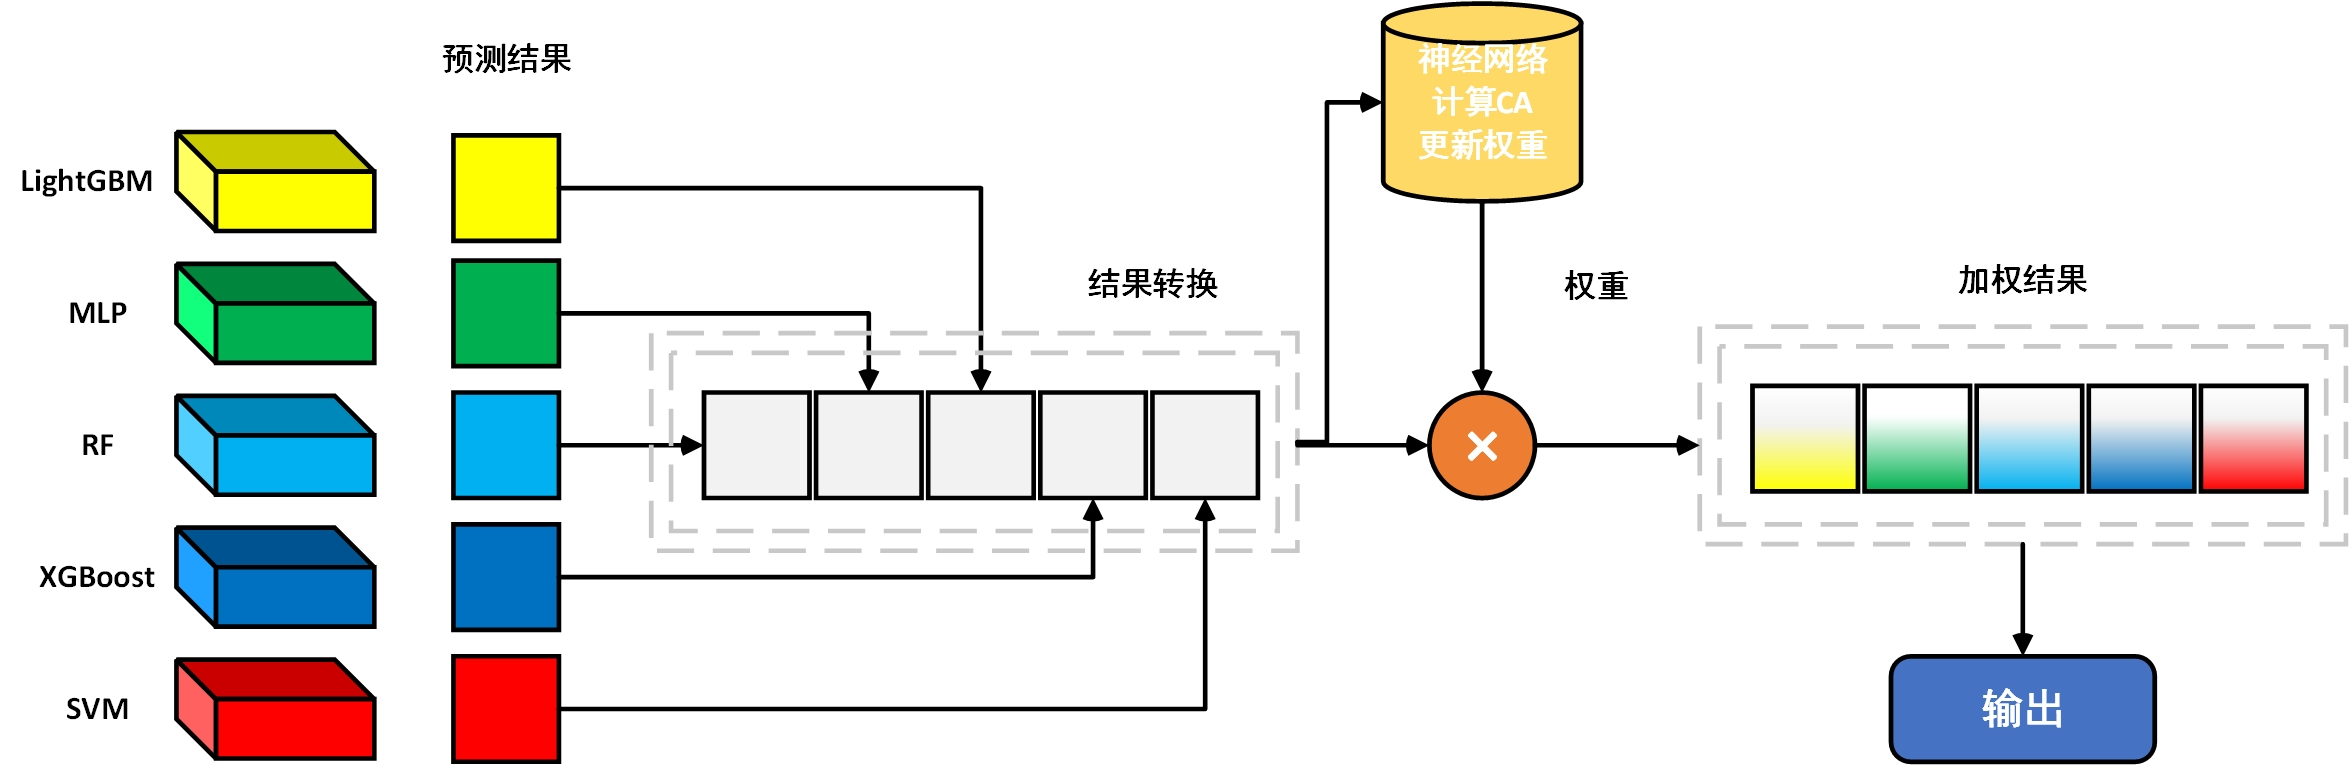
\includegraphics[width=.82\textwidth]{通道注意力加权流程图.jpg}
					\caption{CA加权集成学习流程图}
					\label{fig:5}
				\end{figure}
				
				
			\subsubsection{模型建立与求解}
				\textbf{一、判断患者是否发生血肿扩张}
				
				我们通过使用Python读入,对数据表1、数据表2相关字段经过检查,未发现缺失值,所以无需做缺失值处理。表1发现三位患者数据出现异常已经在本文\ref{sec:4.1.1}部分进行解释处理,此处不做赘述,经过计算以及\ref{sec:4.1.1}部分的判断依据,我们获得了前100位患者是否发生血肿扩张情况的结果,其中出现了\textbf{7位患者具有异常判断结果},他们分别是\textbf{sub008、sub015、sub016、sub025、sub034、sub052、sub063}。
				
				按照分析中所说,我们对7位患者是否发生血肿情况进行定量预测,首次检测到随访1区间内患者基于短期数据预测结果如下:
				
				\begin{table}[H]
					\centering
					\begin{tabular}{|c|c|c|c|c|c|c|}
						\hline
						\rowcolor{green!30} ID & 90天mRS & 年龄 & α(h) & 变化率(mL/h) & 发生时间(h) & 是否发生扩张 \\ \hline
						\rowcolor{green!5}sub008 & 4  & 55  & 2.00  & 0.7129 & 10.41 & 1 \\ \hline
						\rowcolor{white!5}sub015 & 2  & 81  & 5.00  & 0.0446 & 139.53 & 0 \\ \hline
						\rowcolor{green!5}sub016 & 5  & 61  & 1.00  & 0.0093 & 646.16 & 0 \\ \hline
						\rowcolor{white!5}sub025 & 2  & 38  & 7.00  & 0.475 & 19.63 & 1 \\ \hline
						\rowcolor{green!5}sub034 & 4  & 52  & 0.50  & -0.0078 & 0 & 0 \\ \hline
						\rowcolor{white!5}sub052 & 3  & 77  & 4.00  & 0.8126 & 11.38 & 1 \\ \hline
						\rowcolor{green!5}sub063 & 2  & 61  & 10.00  & 0.0437 & 147.29 & 0 \\ \hline
					\end{tabular}
				\end{table}
				
				将异常结果填入答案后,我们获得了最终的答案,我们将48h内未发生扩张情况的患者血肿扩张时间设定为0,此处仅输出10行答案作为展示:
				
				\begin{table}[H]
					\centering
					\setlength{\tabcolsep}{13mm}
					\begin{tabular}{|c|c|c|}
						\hline
						\rowcolor{blue!25} ID & 是否发生血肿扩张 & 血肿扩张时间 \\ \hline
						\rowcolor{blue!5}sub001 & 0 & 0\\ \hline
						\rowcolor{white!5}sub003 & 1 & 9.52\\ \hline
						\rowcolor{blue!5}sub008 & 1 & 10.41\\ \hline
						\rowcolor{white!5}sub009 & 1  & 40.06 \\ \hline
						\rowcolor{blue!5}sub015 & 0  & 0  \\ \hline
						\rowcolor{white!5}sub052 & 1  & 11.38 \\ \hline
						\rowcolor{blue!5}sub061 & 1  & 6.54 \\ \hline
						\rowcolor{white!5}sub076 & 1  & 15.99 \\ \hline
						\rowcolor{blue!5}sub079 & 1  & 27.85 \\ \hline
						\rowcolor{white!5}sub099 & 1  & 17.67 \\ \hline
					\end{tabular}
				\end{table}
				
				患者的血肿扩张情况整体占比如图\ref{fig:6}所示:
				
				\begin{figure}[H]
					\centering
					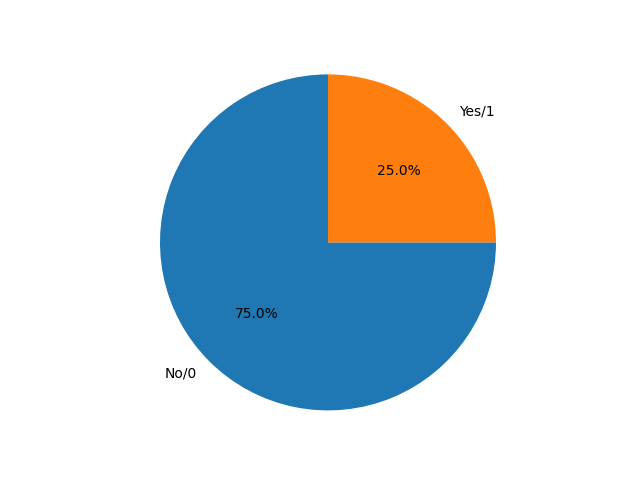
\includegraphics[width=.82\textwidth]{1a饼图.png}
					\caption{100名患者血肿扩张情况饼图}
					\label{fig:6}
				\end{figure}
				
				
				\textbf{二、预测所有患者发生血肿扩张概率}
				
				我们将上题中的前100位患者的血肿扩张结果拼接其他数据后生成了样本量为100的训练数据集,我们注意到此处没有缺失值,无需做缺失值处理,同时我们注意到性别为男或女,且血压中高压和低压放在了一起,此类特征并不适合模型训练,所以我们将性别转化为0或1,血压分为高压和低压。
				
				经过合适的特征变换,以及针对血肿体积特征采用3$\sigma$拉伊达原理进行异常值的分析处理并采用Min-Max进行标准化后,我们将训练数据输入到模型中,我们通过充分实验,得到了集成学习模型与单个模型的结果,其模型输出的预测概率与真实标签在评估指标\textbf{Accuracy、AUC、F1}评价下的结果如表\ref{tab:3}所示:
				
				\begin{table}[H]
					\centering
					\caption{1b模型训练结果对比}
					\label{tab:3}
					\setlength{\tabcolsep}{7mm}
					\begin{tabular}{|c|c|c|c|}
						\hline
						\rowcolor{green!30} Model & Accuracy & AUC & F1 \\ \hline
						\rowcolor{green!5}LightGBM & 0.75  & 0.428571429 & 0.28\\ \hline
						\rowcolor{white!5}MLP & 0.70  & 0.722380952
						  & 0.40  \\ \hline
						\rowcolor{green!5}RF & 0.71  & 0.404761905
						  & 0.13  \\ \hline
						\rowcolor{white!5}SVC & 0.72  & 0.511904762
						  & 0.10  \\ \hline
						\rowcolor{green!5}XGBoost & 0.71  & 0.428571429
						  & 0.15  \\ \hline
						\rowcolor{white!5}CA加权集成学习 & \textbf{0.81}  & \textbf{0.778251852}  & \textbf{0.58}  \\ \hline
					\end{tabular}
				\end{table}
				
				我们可以看到通过Channel Attention通道注意力机制学习到的权值参数在集成学习时施加到不同算法结果上,对整体模型的预测效果有了明显的提升,我们将权重参数输出,得到加权学习模型最终的权重分布如公式所示(仅展示效果,权重仅保留4位有效数字):
				
				\begin{equation}
					\centering
					\begin{aligned} 
						\varphi(x)=A_{LightGBM}(x)\cdot 0.3545+A_{MLP}(x)\cdot 0.3063+A_{RF}(x)\cdot 0.1070 \\ +A_{SVC}(x)\cdot 0.1298+A_{XGBoost}(x)\cdot 0.2549
					\end{aligned}
				\end{equation}
				
				其中五个集成学习子模型输出的预测情况对比如图\ref{fig:7}所示。
				
				\begin{figure}[H]
					\centering
					\caption{子模型预测对比}
					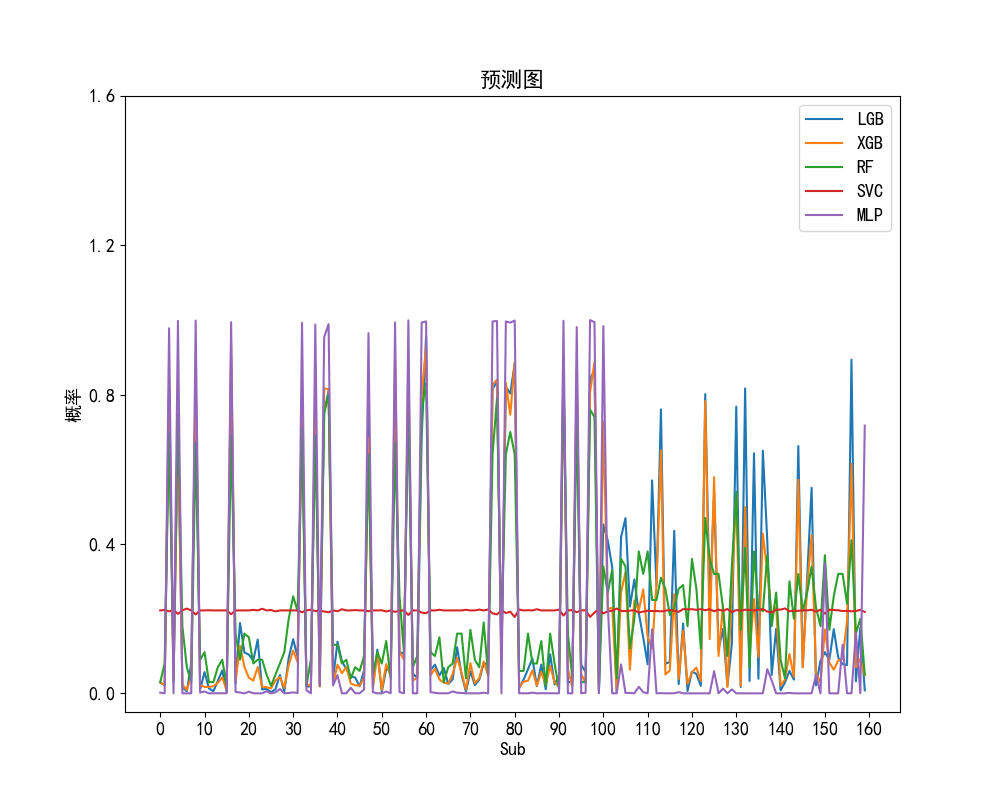
\includegraphics[width=.60\textwidth]{1b预测对比图.png}
					\label{fig:7}
				\end{figure}
				
				最后,集成模型输出的160位患者是否发生血肿扩张的概率结果如表\ref{tab:5}所示(仅展示其中的10位患者结果):
				
				\begin{table}[H]
					\centering
					\caption{1b答案展示}
					\label{tab:5}
					\setlength{\tabcolsep}{17mm}
					\begin{tabular}{|c|c|}
						\hline
						\rowcolor{blue!25} ID & 血肿扩张预测概率 \\ \hline
						\rowcolor{blue!5}sub001 & 0.0177 \\ \hline
						\rowcolor{white!5}sub002 & 0.1200 \\ \hline
						\rowcolor{blue!5}sub003 & 0.9701 \\ \hline
						\rowcolor{white!5}sub004 & 0.0533  \\ \hline
						\rowcolor{blue!5}sub005 & 0.9950  \\ \hline
						\rowcolor{white!5}sub006 & 0.0248  \\ \hline
						\rowcolor{blue!5}sub007 & 0.0328  \\ \hline
						\rowcolor{white!5}sub008 & 0.0235 \\ \hline
						\rowcolor{blue!5}sub009 & 0.9027  \\ \hline
						\rowcolor{white!5}sub010 & 0.0159  \\ \hline
					\end{tabular}
				\end{table}
				
							
		
		\subsection{【问题二】血肿周围水肿进展和治疗关联探索}
			\subsubsection{问题分析2a:全体患者水肿体积随时间进展曲线拟合}
				首先,题目要求我们通过学习前100名患者水肿体积随时间间变化的趋势来拟合一条符合全体患者水肿体积随时间进展的曲线,我们需要先获取到前100名患者检查次数,并从每次检查中拿到对应当次水肿体积的信息,我们注意到每次检查的时间信息都是完整的时间类型不方便计算,且每名患者的每次检查时间从早到晚均有分布,倘若全部放入$X$轴,会将区间拉的非常稀疏,所以我们首先考虑\textbf{将完整时间类型转换为——与首次检查所间隔时间},同时我们将水肿体积也重新转换单位统一成了mL,数据还需要做异常值的判断,经过完整的数据处理工作后,我们就能获得用于拟合曲线的数据,数据表如表\ref{tab:6}所示。
				
				\begin{table}[H]
					\caption{水肿体积随时间变化表(头部部分数据)}
					\label{tab:6}
					\rowcolors{2}{gray!10}{white}
					\begin{tabular}{ccc}
						\toprule[1.5pt]
						\makebox[0.3\textwidth][c]{ID} &
						\makebox[0.3\textwidth][c]{Time(h)} & \makebox[0.4\textwidth][c]{Volume(mL)} \\
						\midrule[1pt]
						sub1 & 2.50 & 48.919\\
						sub1 & 8.26 & 57.898\\
						sub1 & 132.10 & 81.747\\
						sub1 & 259.73 & 107.793\\
						sub1 & 425.53 & 126.558\\
						sub2 & 3.00 & 23.526\\
						sub2 & 14.92 & 23.39\\
						\bottomrule[1.5pt]
					\end{tabular}			
				\end{table}
				
				拟合曲线通常做法是进行回归分析,确定实验数据之间的线性关系,但现实数据之间不一定是线性关系,更可能是复杂的非线性关系,所以此时用函数曲线拟合可以更准确的描述实验现象,寻找数据内在的规律。我们考虑到可以使用多种函数来完成拟合曲线,分别采用\textbf{线性拟合、二次多项式拟合、四次多项式拟合、高斯拟合对比最终曲线结果},来找到全体患者水肿体积随时间进展的最佳描述曲线,并计算到真实值与曲线间的残差。
				
			\subsubsection{问题分析2b:人群亚组划分与曲线拟合}
				该题要求我们找到患者水肿体积随时间进展的个体差异,根据不同人群的个体差异构建水肿体积变化亚组,再按照不同的亚组重新构建拟合曲线,并计算组内真实值与曲线间的残差。
				
				我们注意到,该题的一大难点是每位患者的数据有多个时间对应的多个水肿体积信息,这些信息应该是属于个人的,用于体现水肿体积变化,所以是高度不可分的,而亚组的分组依据理应就是组内患者具有类似的水肿变化情况,所以直接将2a中的数据表进行聚类分析是错误的,我们考虑找到一种办法来高度抽象每个患者的水肿变化情况,将多条不同时间点的水肿体积数据转化为一条体现水肿变化率的数据。我们将患者多次检查的水肿体积变化与时间做商,得到不同时期下的水肿变化率,再\textbf{通过统计分析获得每位患者水肿变化率的均值和标准差情况,来高度概括这名患者水肿体积随时间变化的特征},依据该特征我们就能很方便的对多名患者进行\textbf{K-Means聚类分析},变化后的训练数据如表\ref{tab:7}所示。
				
				\begin{table}[H]
					\caption{患者水肿变化特征表(部分数据)}
					\label{tab:7}
					\rowcolors{2}{gray!10}{white}
					\begin{tabular}{ccc}
						\toprule[1.5pt]
						\makebox[0.3\textwidth][c]{ID} &
						\makebox[0.3\textwidth][c]{Mean} & \makebox[0.4\textwidth][c]{Standard} \\
						\midrule[1pt]
						sub1 & 0.516609 & 0.694506\\
						sub10 & 0.114889 & 0.265286\\
						sub100 & -0.028230 & 0.015190\\
						sub12 & 0.034121 & 0.132560\\
						\bottomrule[1.5pt]
					\end{tabular}			
				\end{table}
			
			\subsubsection{问题分析2c:治疗方法与水肿体积进展关系}
				该题需要我们分析不同治疗方法对水肿体积进展模式的影响,通常多特征之间的相关性分析主要采用某些相关性系数的计算来定量分析,如:\textbf{Spearman系数、Kendall相关系数、随机森林重要性分析、灰色关联度系数等},治疗方法包括脑室引流、止血治疗、降颅压治疗、降压治疗、镇静镇痛治疗、止吐护胃、营养神经等七个手段,通过与水肿体积进展变化数据进行训练数据的建立,我们考虑\textbf{采用上述多种相关性分析方法对每一个治疗方法与水肿体积进展模式计算相关性,并通过多次随访变化结果计算平均相关性},最终我们便可以充分分析不同治疗方法的或正向或反向的相关影响。
			
			\subsubsection{问题分析2d:血肿、水肿及治疗方法三者之间的关系}
				与2c类似,我们需要分析血肿体积、水肿体积以及治疗方法三者之间的关系。除了上述提到的相关性系数的计算来定量分析特征之间的关系之外,还有一些方法可以帮助我们进行相关性分析,如:\textbf{单因素方差分析、多因素方差分析、热力图等},通过整合多种相关性分析方法的结果,我们就可以对三者之间的关系进行理论分析。
				
				问题二整体流程图如图\ref{fig:16}所示:
				
				\begin{figure}[H]
					\centering
					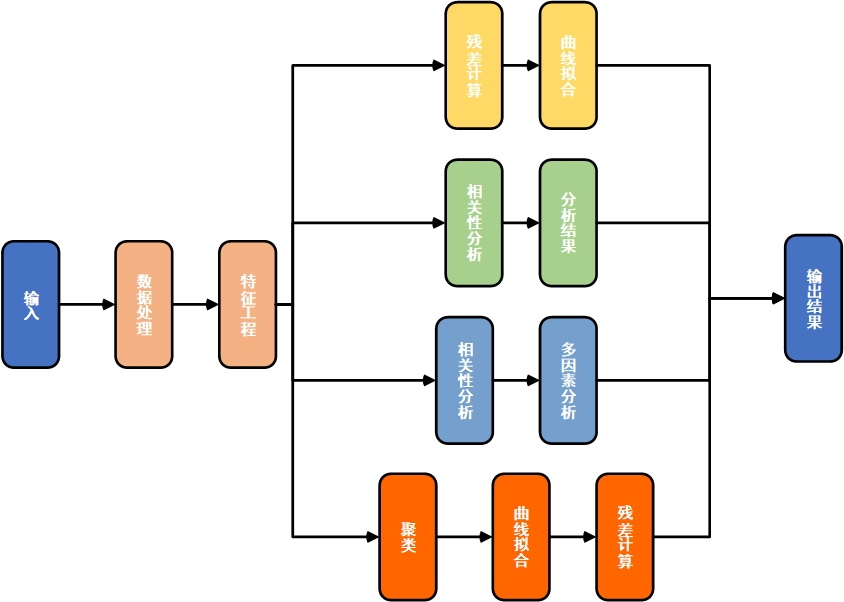
\includegraphics[width=.60\textwidth]{问题二流程图.jpg}
					\caption{问题二流程图}
					\label{fig:16}
				\end{figure}
				
			\subsubsection{模型建立与求解}
				\textbf{一、全体患者曲线拟合}
				
				根据分析,我们获得了用于拟合全体患者曲线的前100位患者水肿体积随时间进展的数据表,我们首先需要整体性的观察一下患者水肿体积与时间的之间的一个分布情况,我们输出患者水肿体积与时间间隔的散点图如图\ref{fig:8}左所示,我们发现数据存在一些离群值,将会导致曲线拟合时拟合到一些不合理的位置,所以我们进行了异常值的剔除,剔除后的效果如图\ref{fig:8}右所示。
				
				\begin{figure}[H]
					\centering
					\subfloat[处理前]{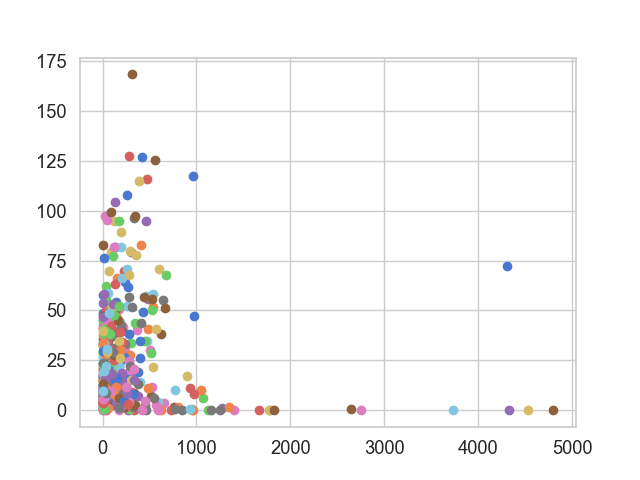
\includegraphics[width=0.45\textwidth]{患者100水肿与时间散点图.png}}\qquad
					\subfloat[处理后]{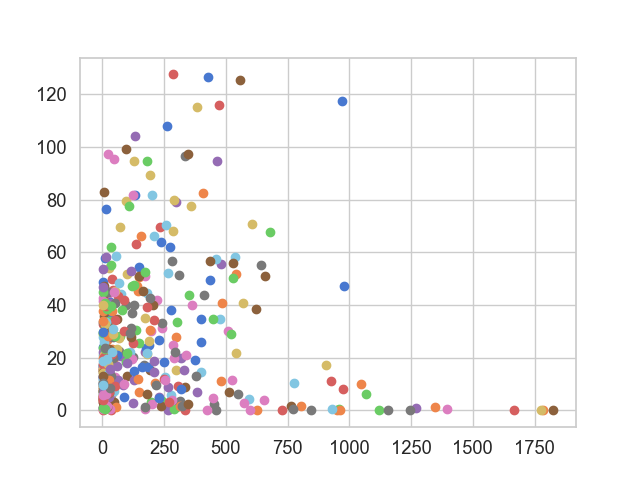
\includegraphics[width=0.45\textwidth]{患者100水肿与时间散点图异常处理后.png}}
					\caption{患者水肿体积与时间散点图}
					\label{fig:8}
				\end{figure}
				
				经过处理后,我们尝试分别使用线性回归、二次多项式回归、四次多项式回归以及高斯拟合对散点进行曲线拟合,分别得到如图\ref{fig:9}结果。
				
				\begin{figure}[htp!]
					\centering
					\subfloat[线性拟合]{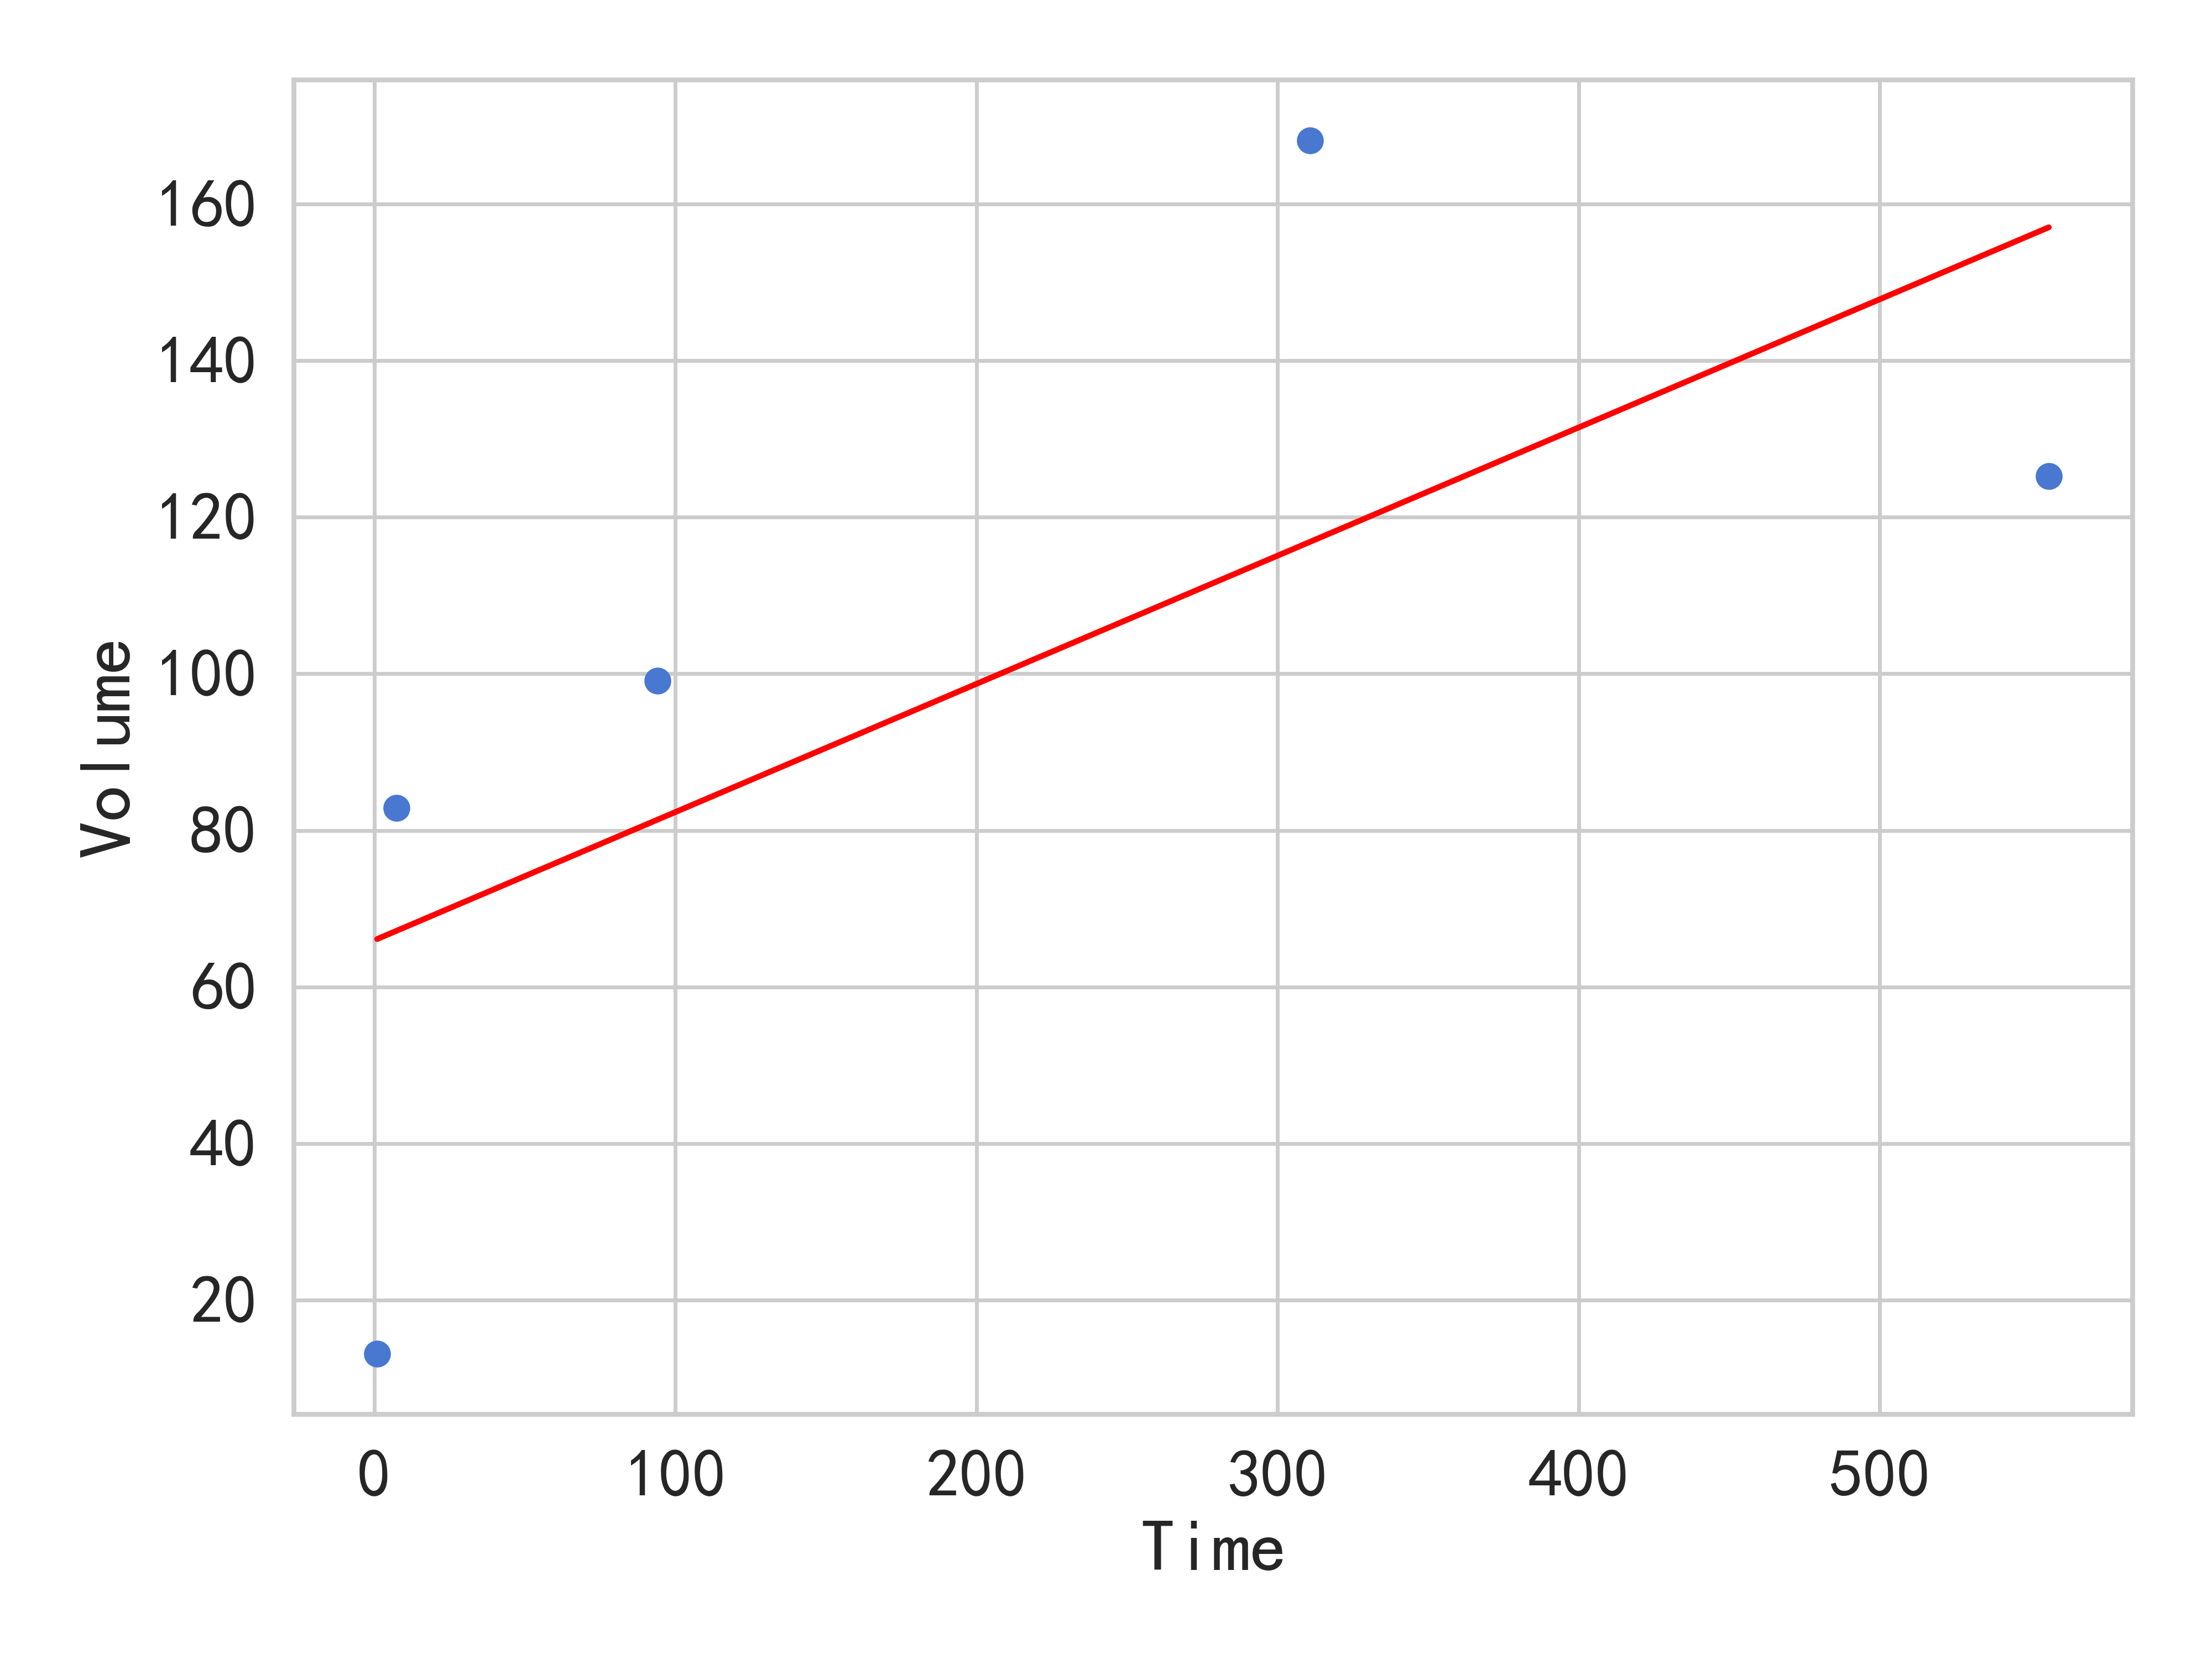
\includegraphics[width=0.40\textwidth]{线性回归散点图.png}}\qquad
					\subfloat[二次多项式拟合]{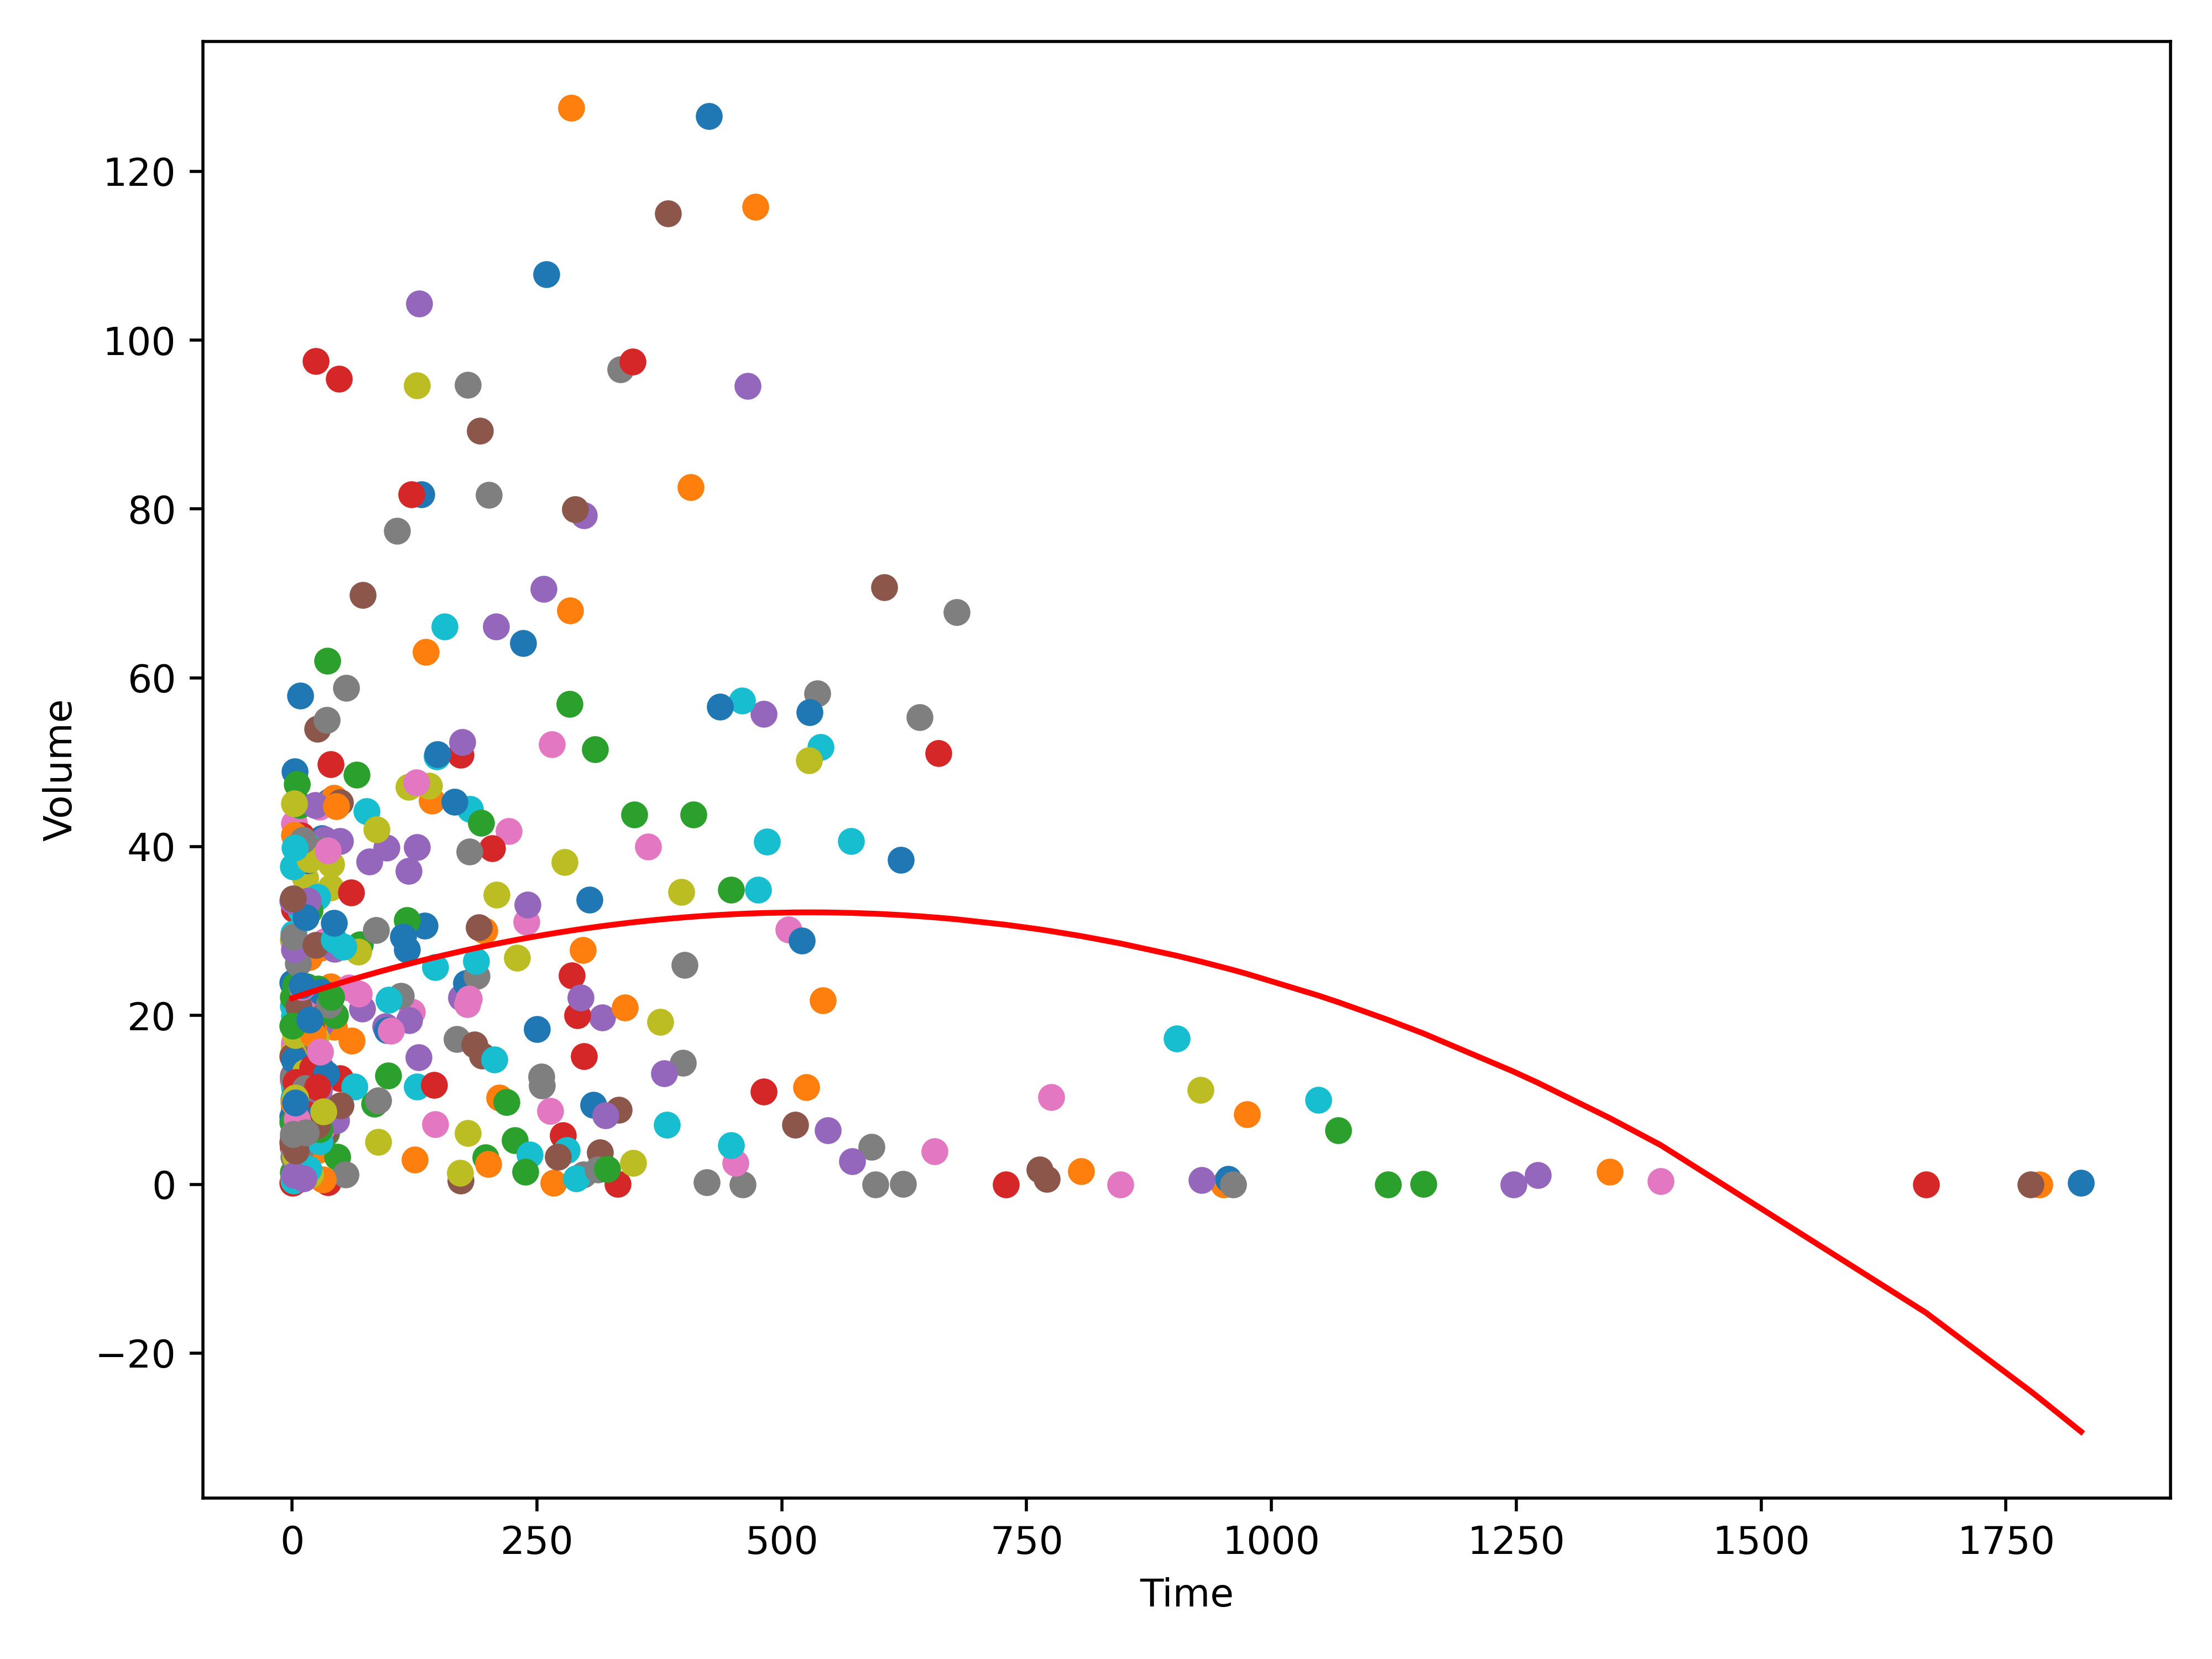
\includegraphics[width=0.40\textwidth]{2次多项式回归散点图.png}} \\
					\subfloat[高斯拟合]{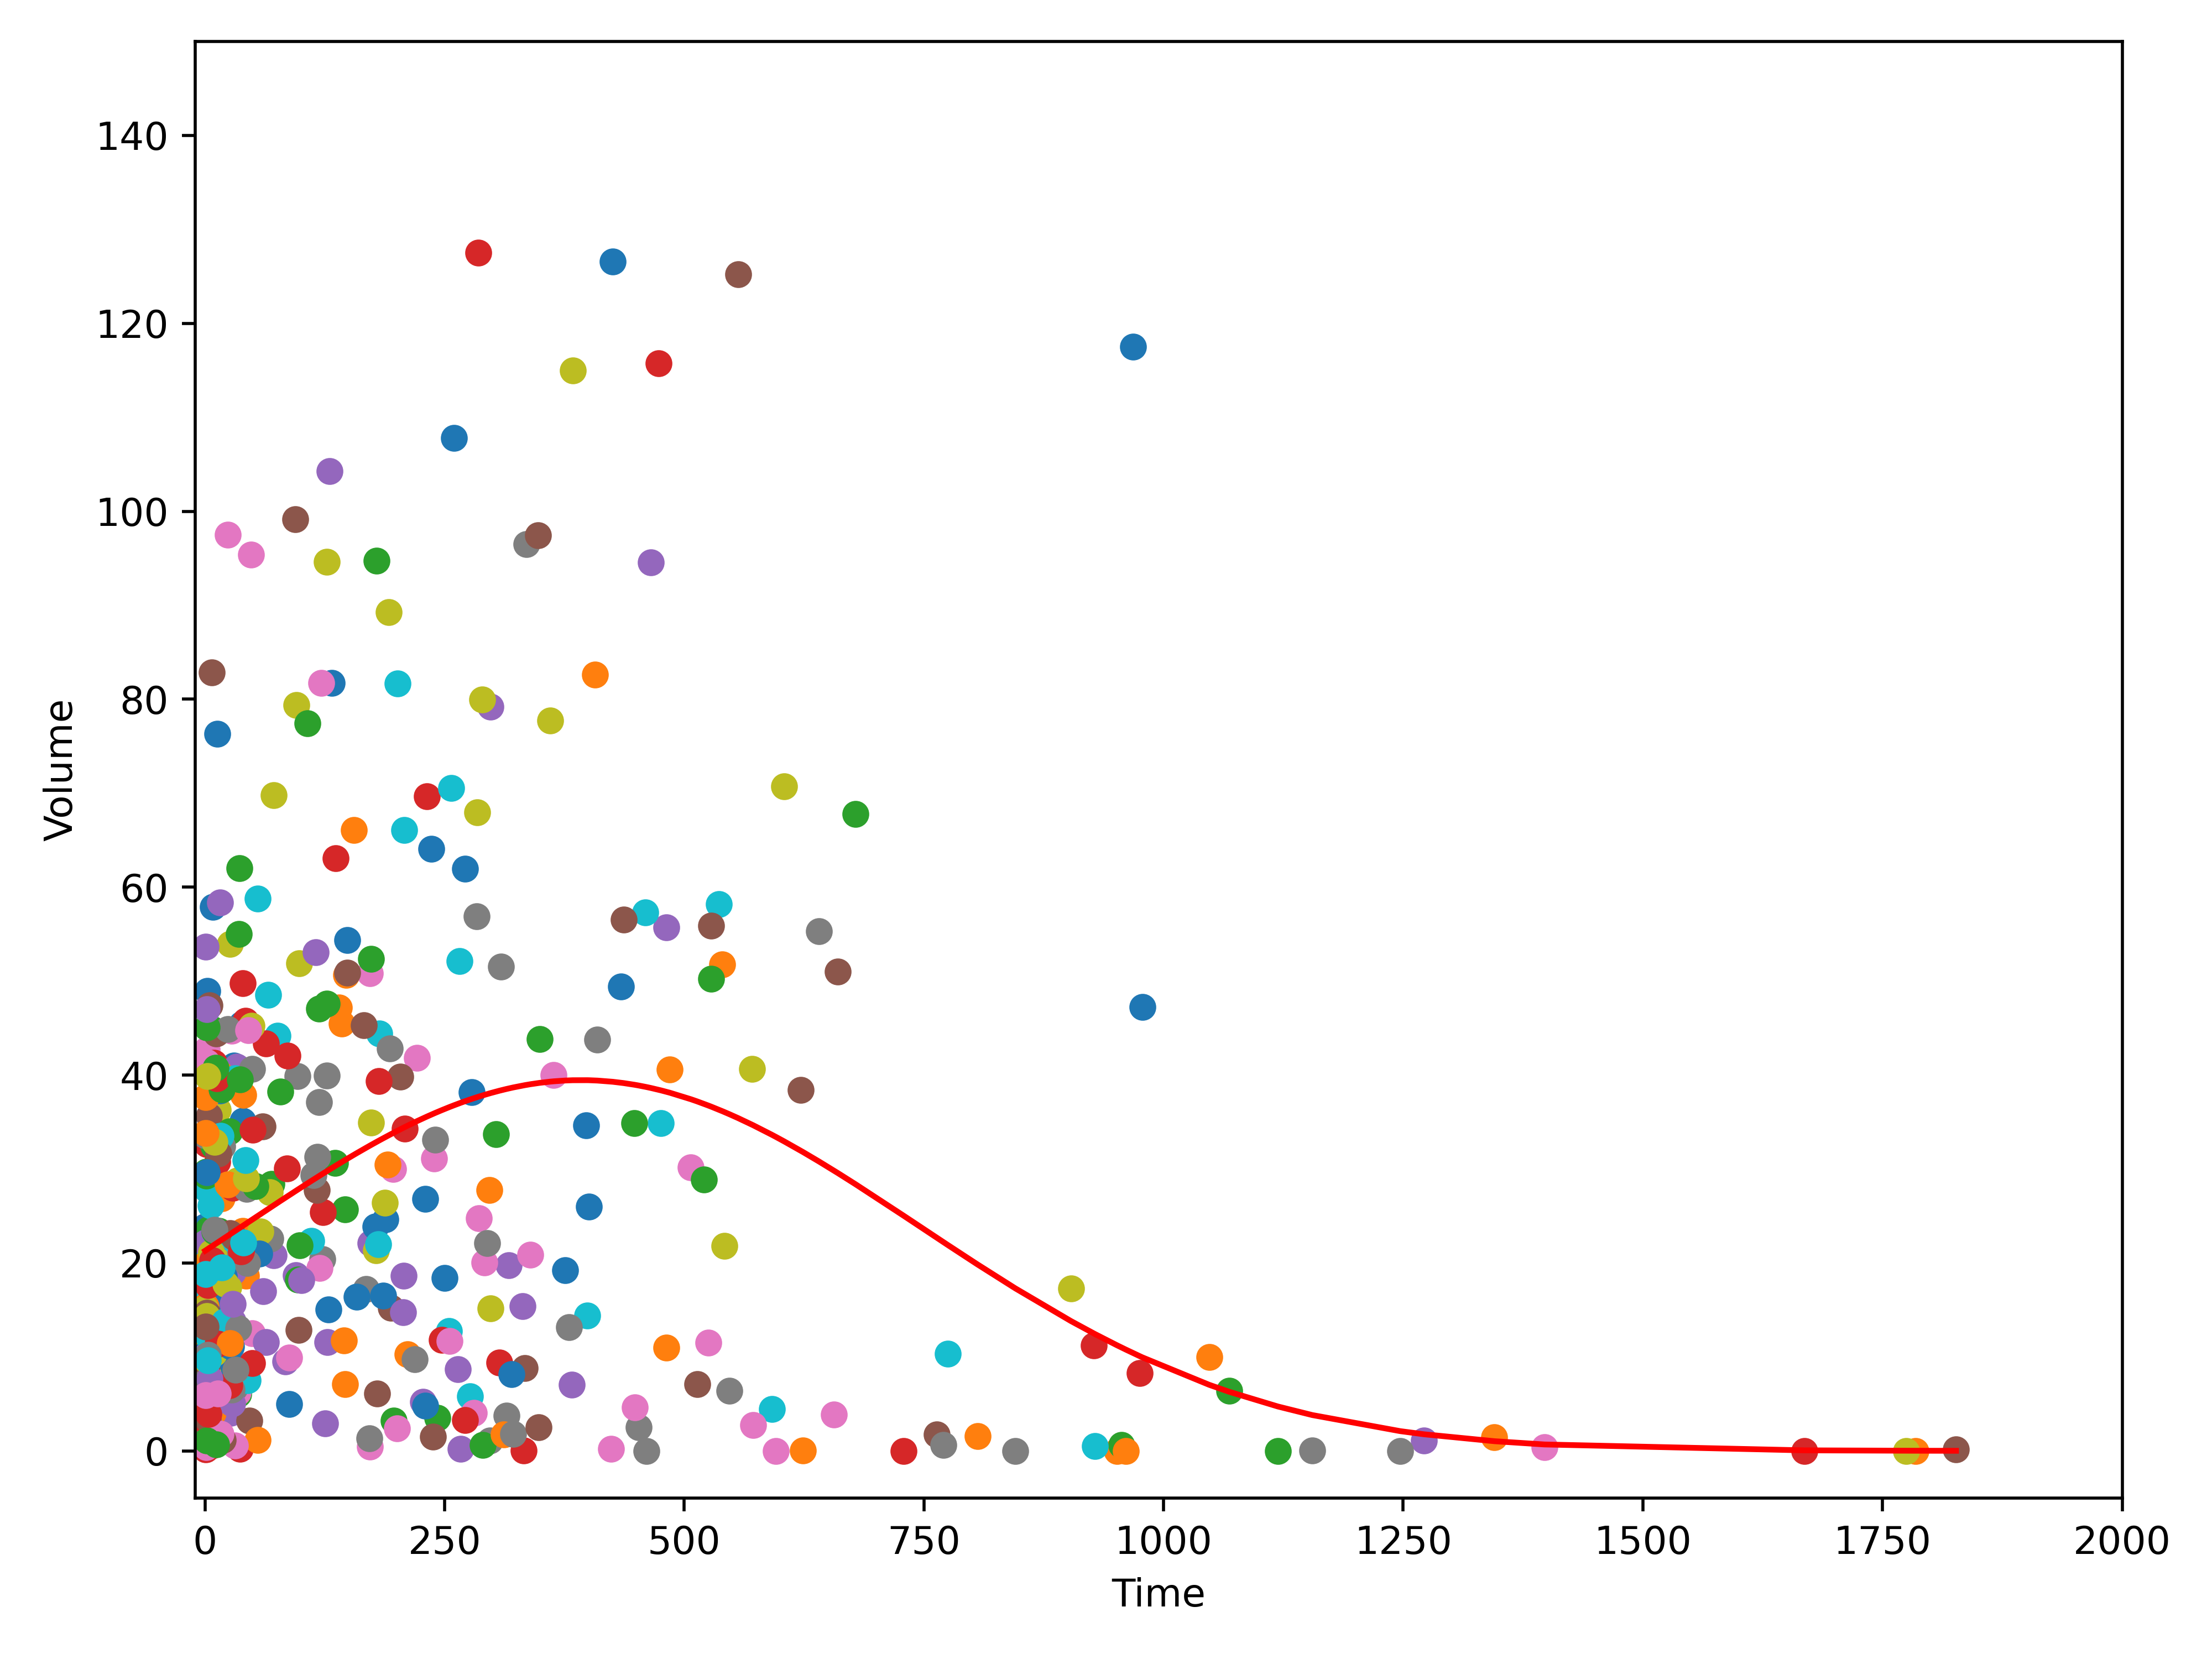
\includegraphics[width=0.40\textwidth]{高斯拟合散点图.png}}\qquad
					\subfloat[四次多项式拟合]{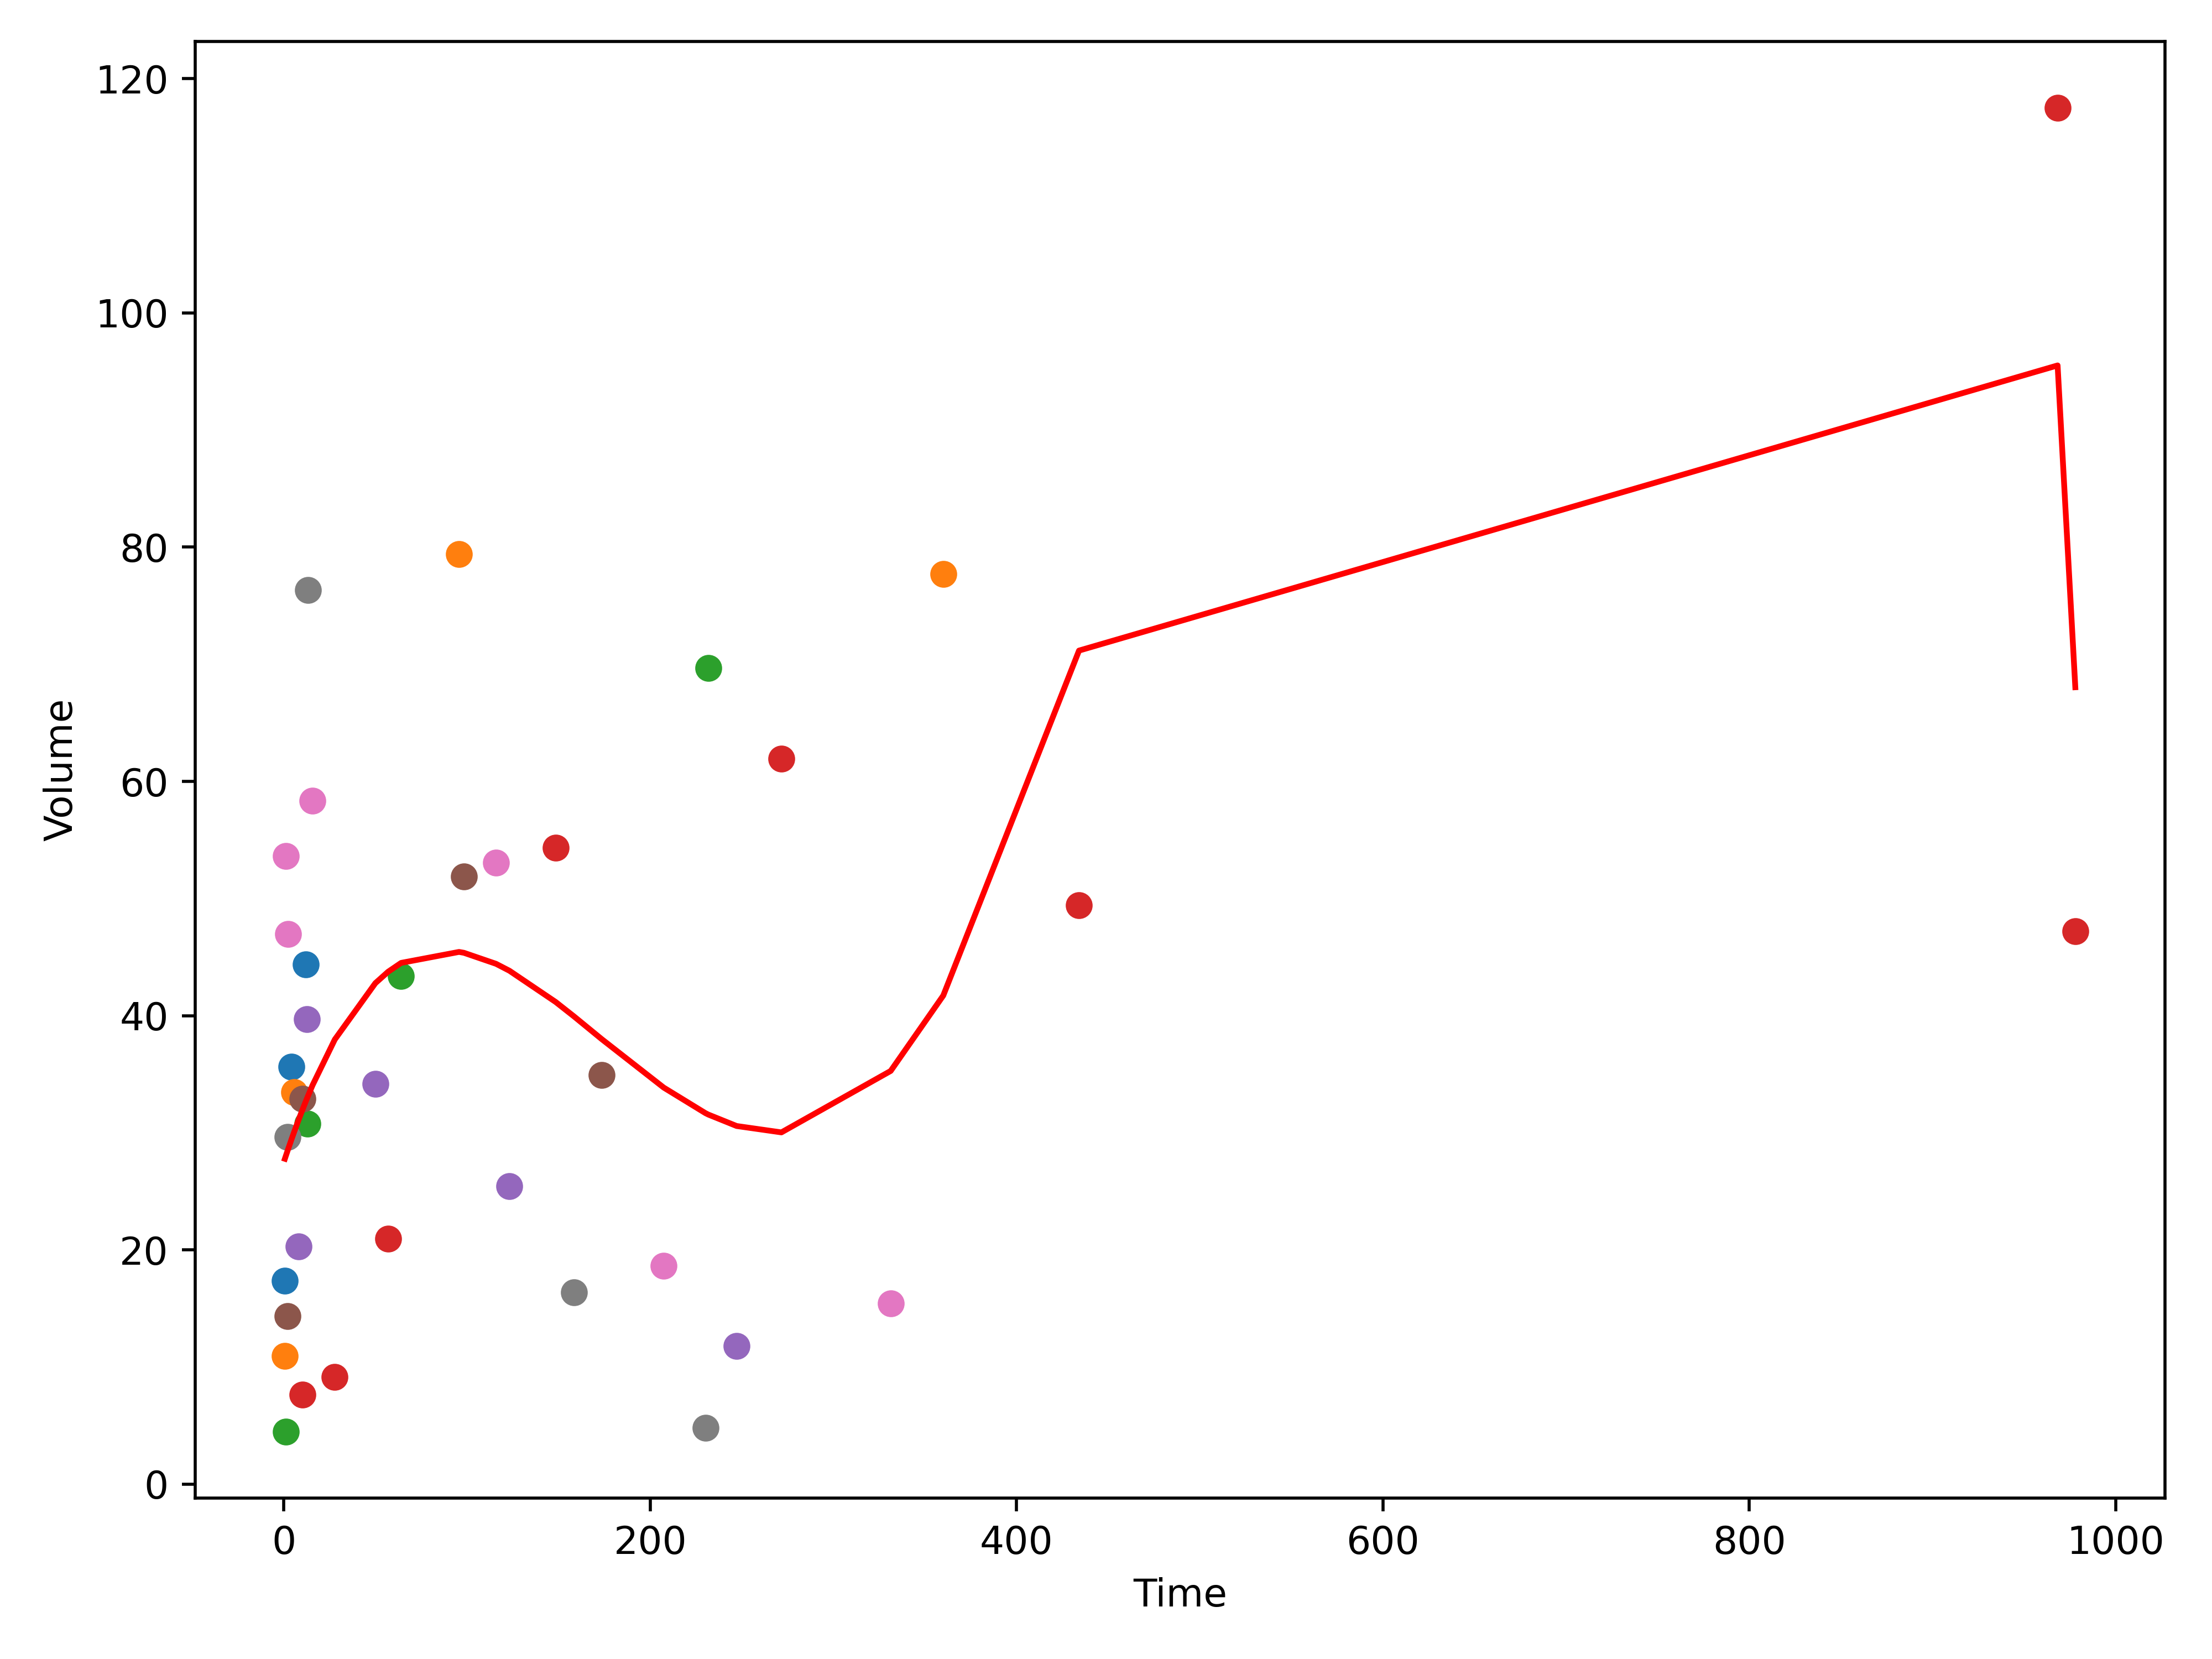
\includegraphics[width=0.40\textwidth]{4次多项式回归散点图.png}}
					\caption{多方法拟合曲线对比}
					\label{fig:9}
				\end{figure}
				
				通过对比四种方法所输出的拟合曲线,我们发现高斯函数与四次多项式函数拟合出来的全体患者水肿体积随时间进展曲线更加贴近患者数据所描述的趋势,同时我们也分别对比输出了四种方式所拟合出来的曲线与真实值之间的平均残差:
				
				\begin{table}[H]
					\caption{四种方法平均残差对比}
					\label{tab:8}
					\rowcolors{2}{gray!10}{white}
					\begin{tabular}{cc}
						\toprule[1.5pt]
						\makebox[0.5\textwidth][c]{Methods} &
						\makebox[0.5\textwidth][c]{Mean Risdual} \\
						\midrule[1pt]
						Linear & 1.83936 \\
						2Polynomial & 1.59432 \\
						4Polynomial & \textbf{1.2626} \\
						Gauss & 1.2911 \\
						\bottomrule[1.5pt]
					\end{tabular}			
				\end{table}
				
				该题要求输出sub001至sub100真实值和所拟合曲线之间存在的残差填写于表4答案中,以附件形式提交,在此不做展示。
				
				\textbf{二、人群亚组划分及曲线拟合}
				
				依据分析如果我们直接对题2a中的散点图进行聚类分析的话,会得到聚类分析图如图\ref{fig:11}左所示结果,这种\textbf{直接聚类结果是不合理的,对于每一个患者来说,不同时期的水肿体积会被割裂开,出现单人多个分组的情况},所以按照分析中的转化方式,我们获得了转化后的针对每位患者水肿变化率描述情况的数据表,数据表散点分布如图\ref{fig:10}所示,可以很明显的观察到三层散点,所以我们尝试\textbf{将K-means聚类中心点设置为3,于是划分出来了3个亚组},每个亚组所包含患者(前100名)如表所示,聚类效果如图\ref{fig:11}右所示。
				
				\begin{figure}[H]
					\centering
					\caption{数据转换后的散点图}
					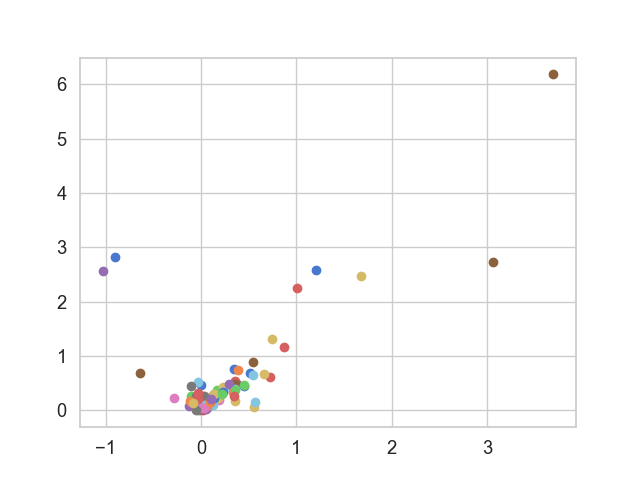
\includegraphics[width=.60\textwidth]{time和volume转换成速度平均值和方差后的散点图.png}
					\label{fig:10}
				\end{figure}
				
				\begin{figure}[H]
					\centering
					\subfloat[数据转换前]{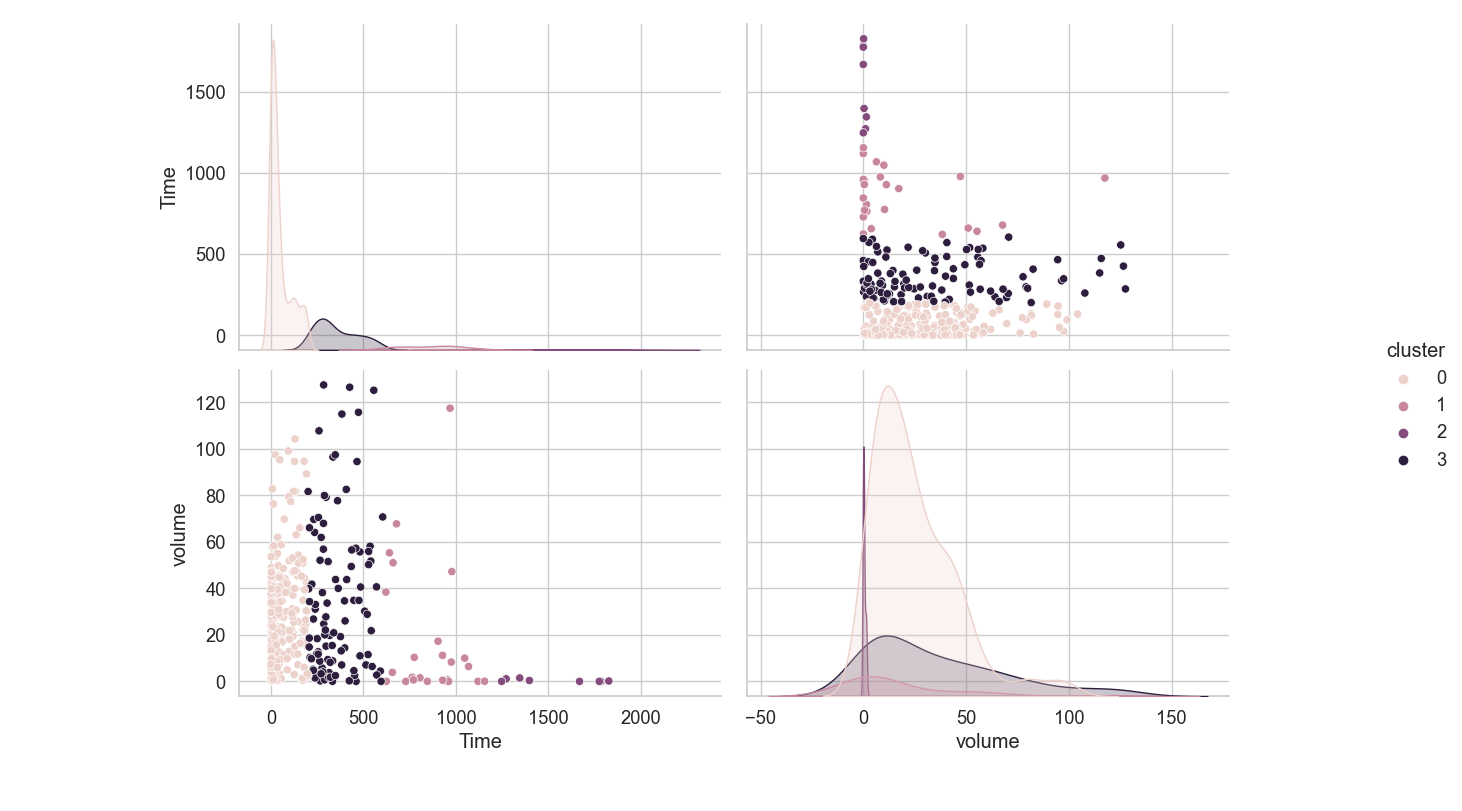
\includegraphics[width=0.55\textwidth]{对散点直接做聚类的分析图.png}}\qquad
					\subfloat[数据转换后]{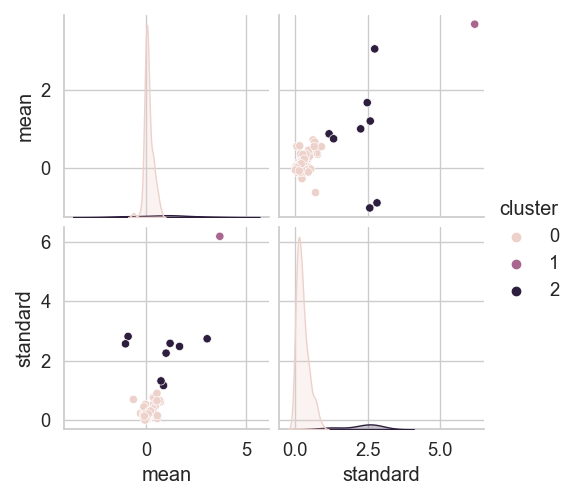
\includegraphics[width=0.35\textwidth]{对散点做特征变换出平均和标准差后做聚类的分析图.png}}
					\caption{患者水肿体积与时间散点图}
					\label{fig:11}
				\end{figure}
				
				\begin{table}[H]
					\centering
					\label{tab:10}
					\caption{患者所属亚组及残差(部分数据)}
					\setlength{\tabcolsep}{13mm}
					\begin{tabular}{|c|c|c|}
						\hline
						\rowcolor{blue!25} ID & 所属亚组 & 残差(亚组) \\ \hline
						\rowcolor{blue!5}sub001 & 0 & -56.21056\\ \hline
						\rowcolor{white!5}sub003 & 0 & -21.42548\\ \hline
						\rowcolor{blue!5}sub008 & 2 & 2.45037\\ \hline
						\rowcolor{white!5}sub095 & 1  & 0.48041 \\ \hline
						\rowcolor{blue!5}sub063 & 2  & 6.42172 \\ \hline
					\end{tabular}
				\end{table}
				
				此时三个亚组所拟合出来的曲线如图\ref{fig:12}所示:
				
				\begin{figure}[H]
					\centering
					\subfloat[亚组0]{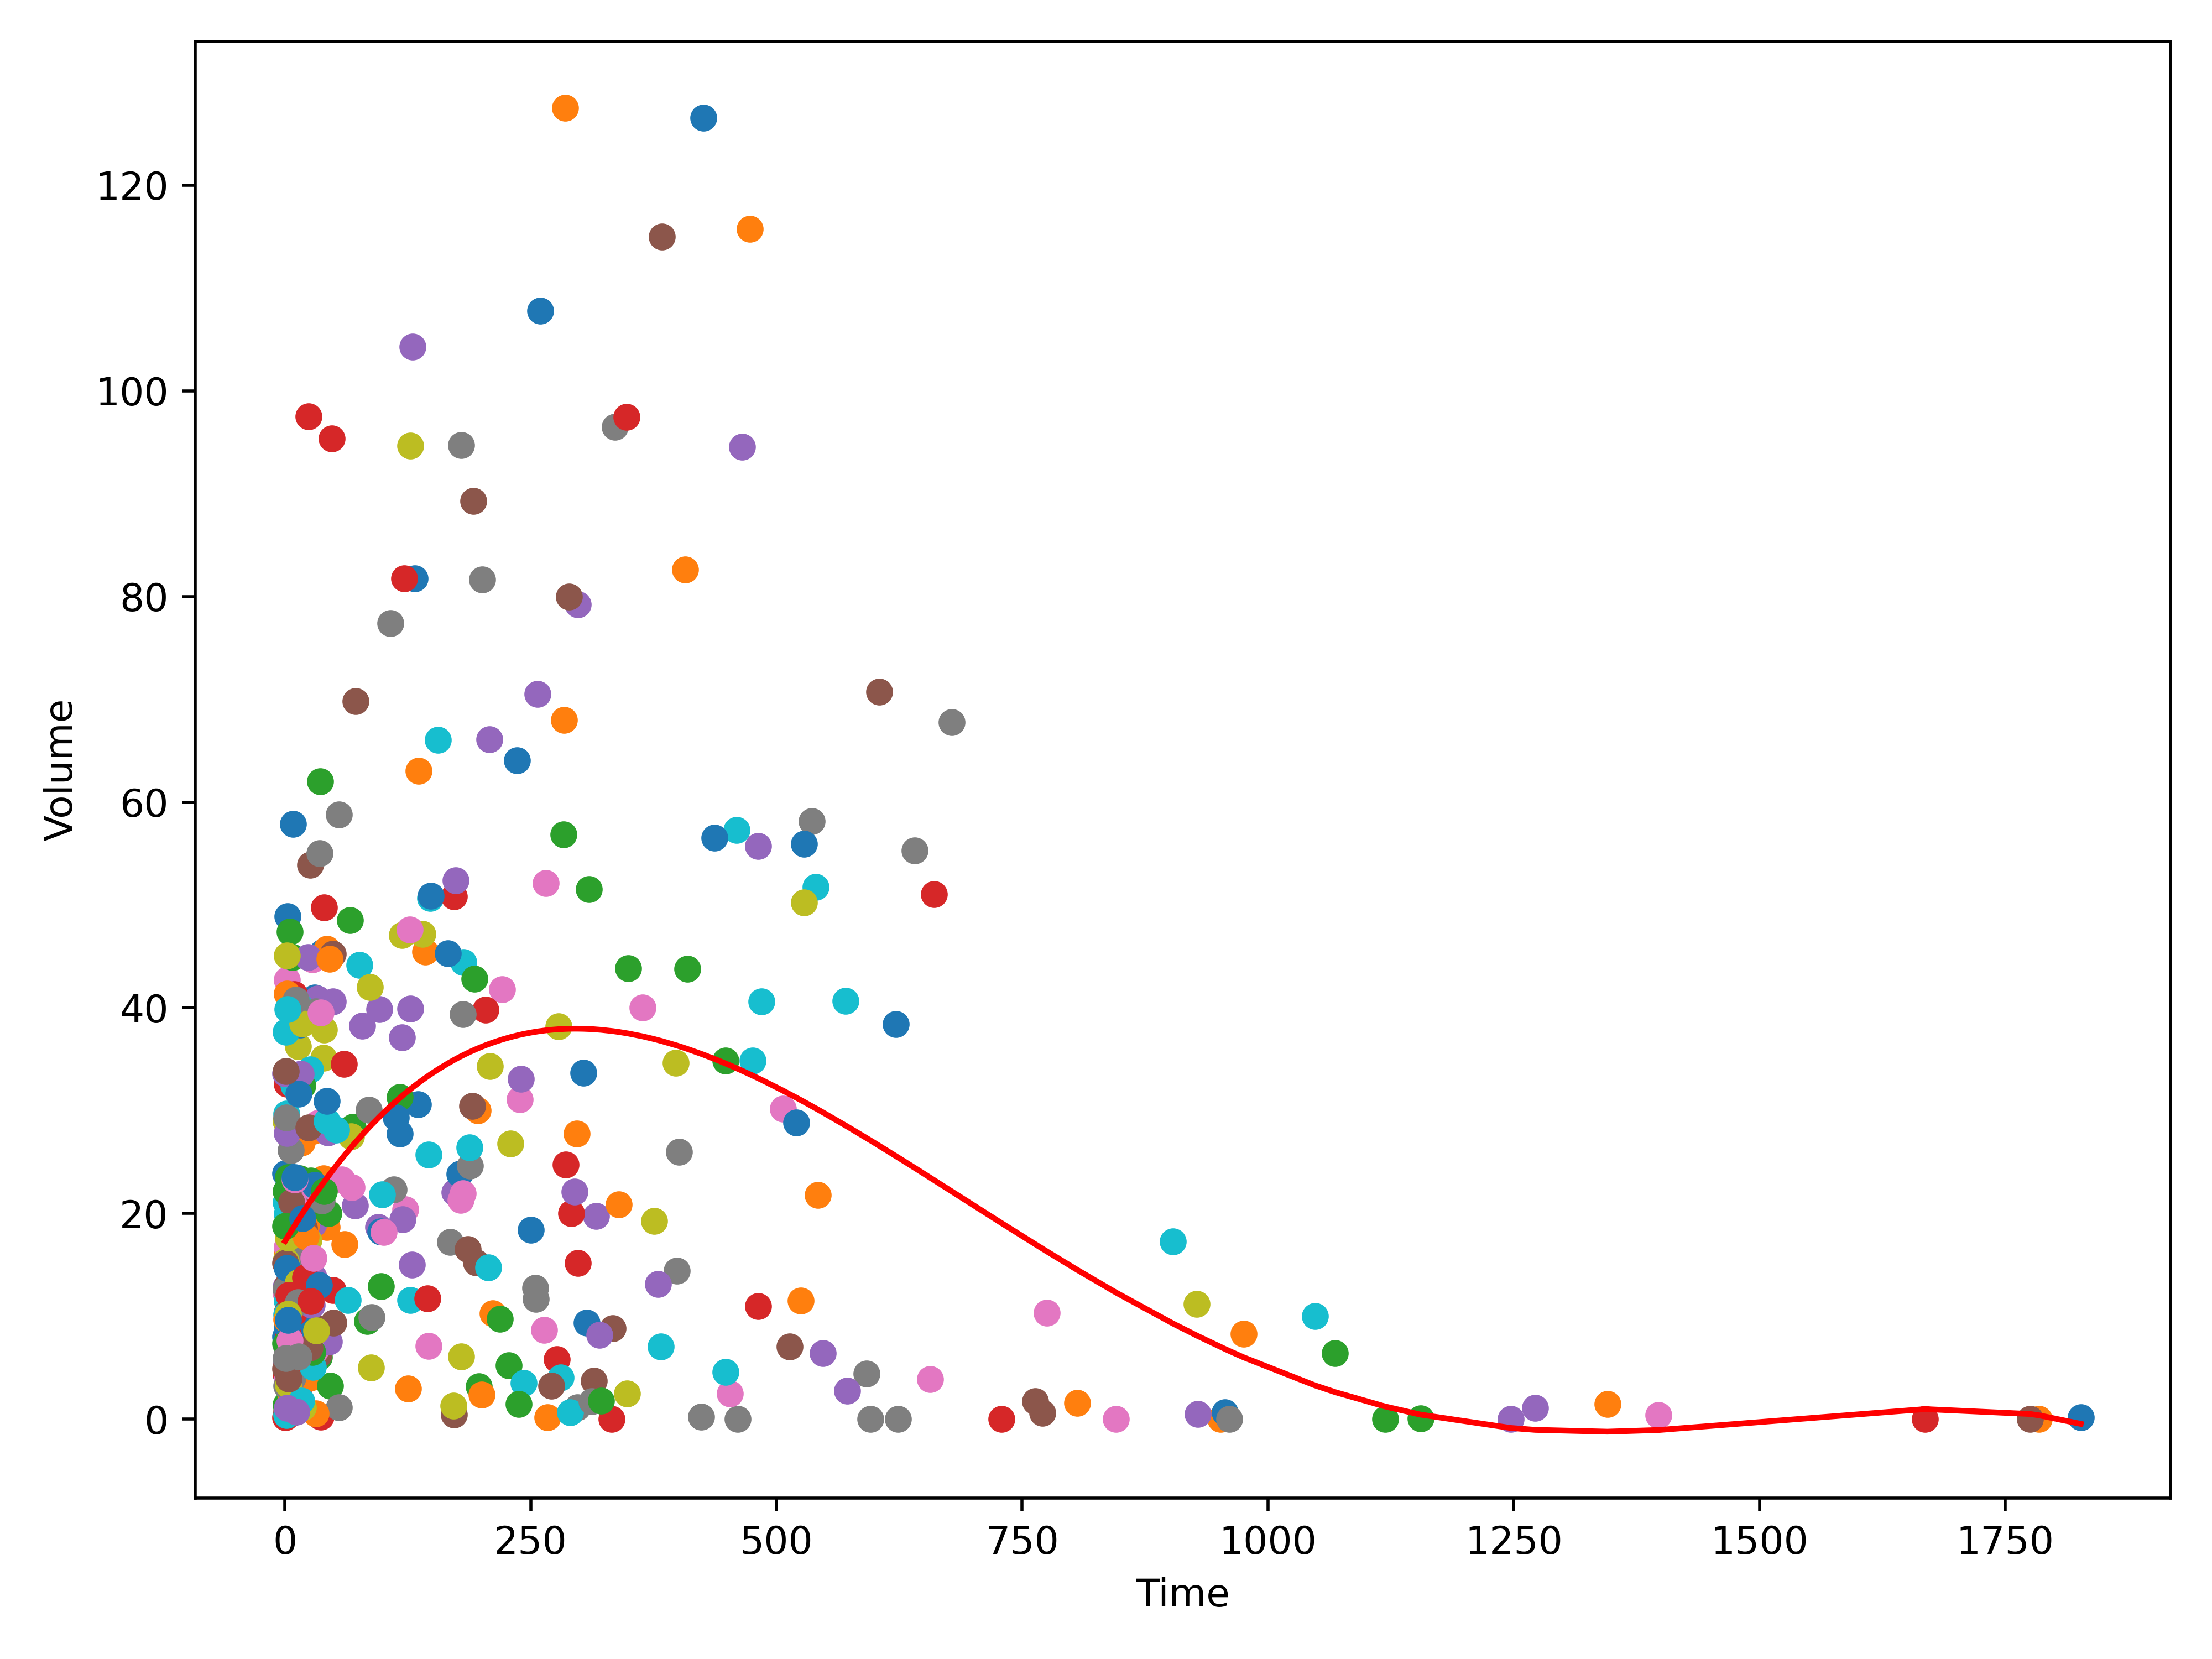
\includegraphics[width=0.34\textwidth]{class04次多项式回归散点图.png}}\qquad
					\subfloat[亚组1]{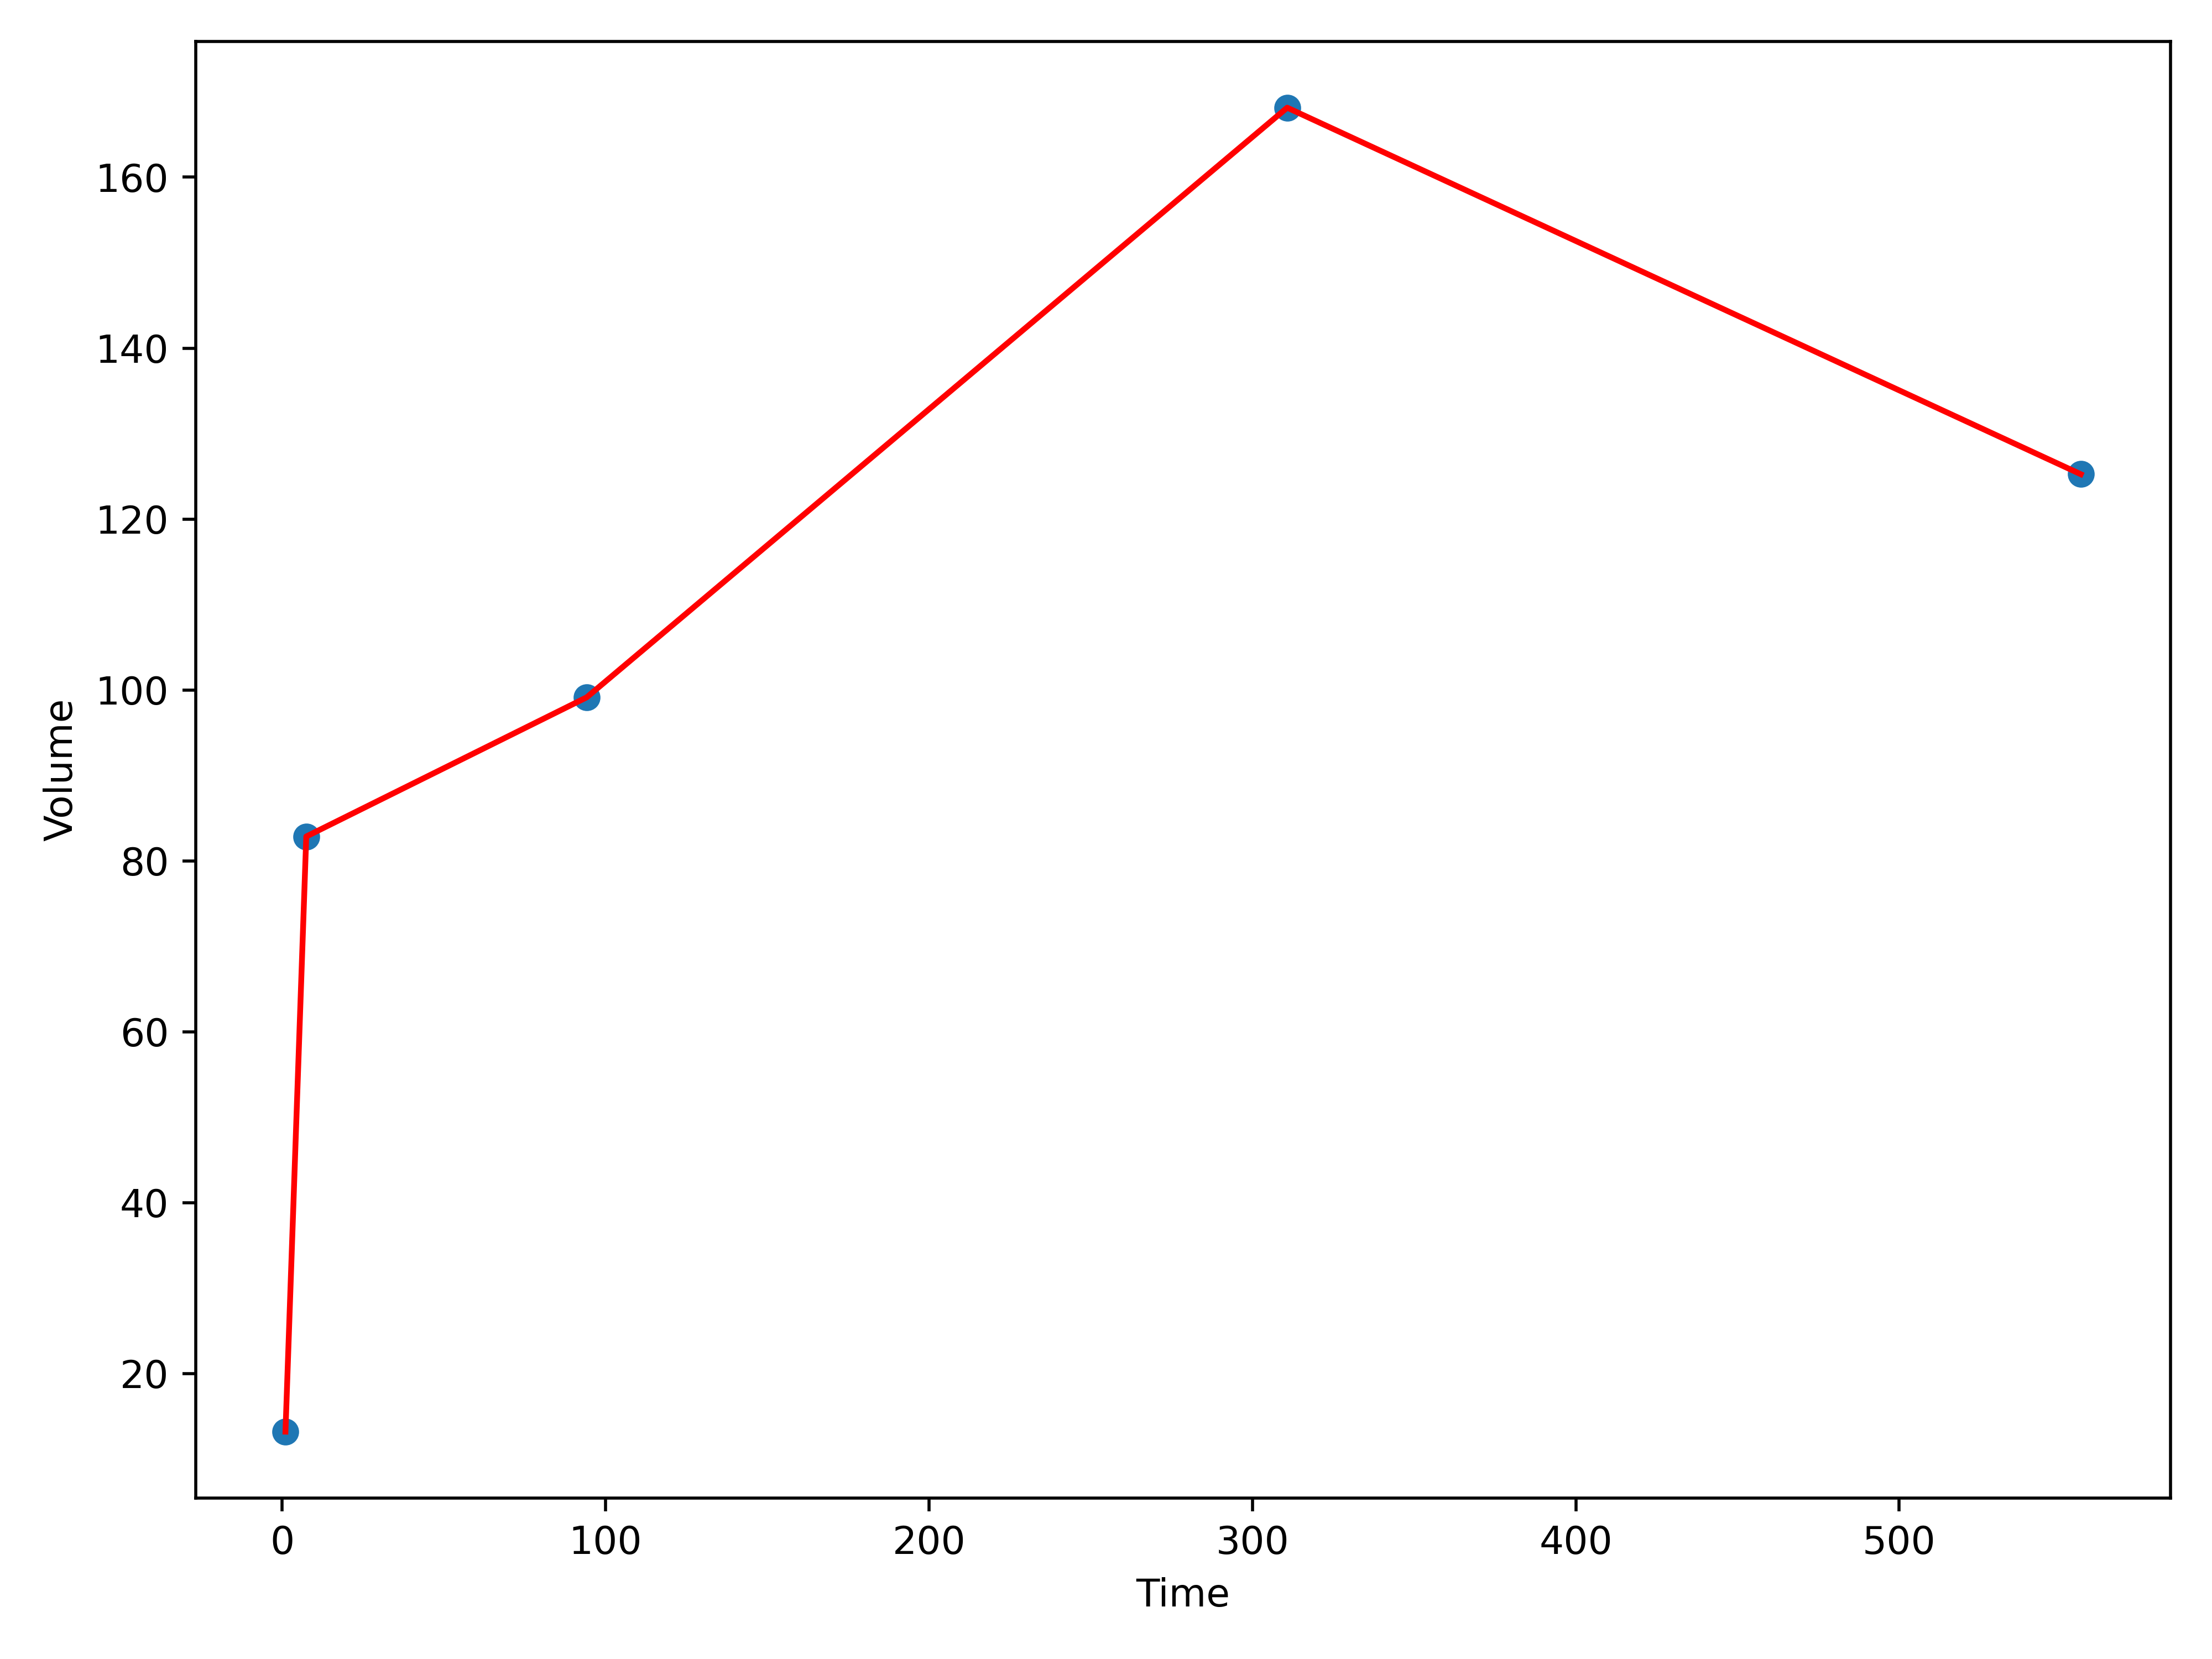
\includegraphics[width=0.33\textwidth]{class14次多项式回归散点图.png}}\qquad
					\subfloat[亚组2]{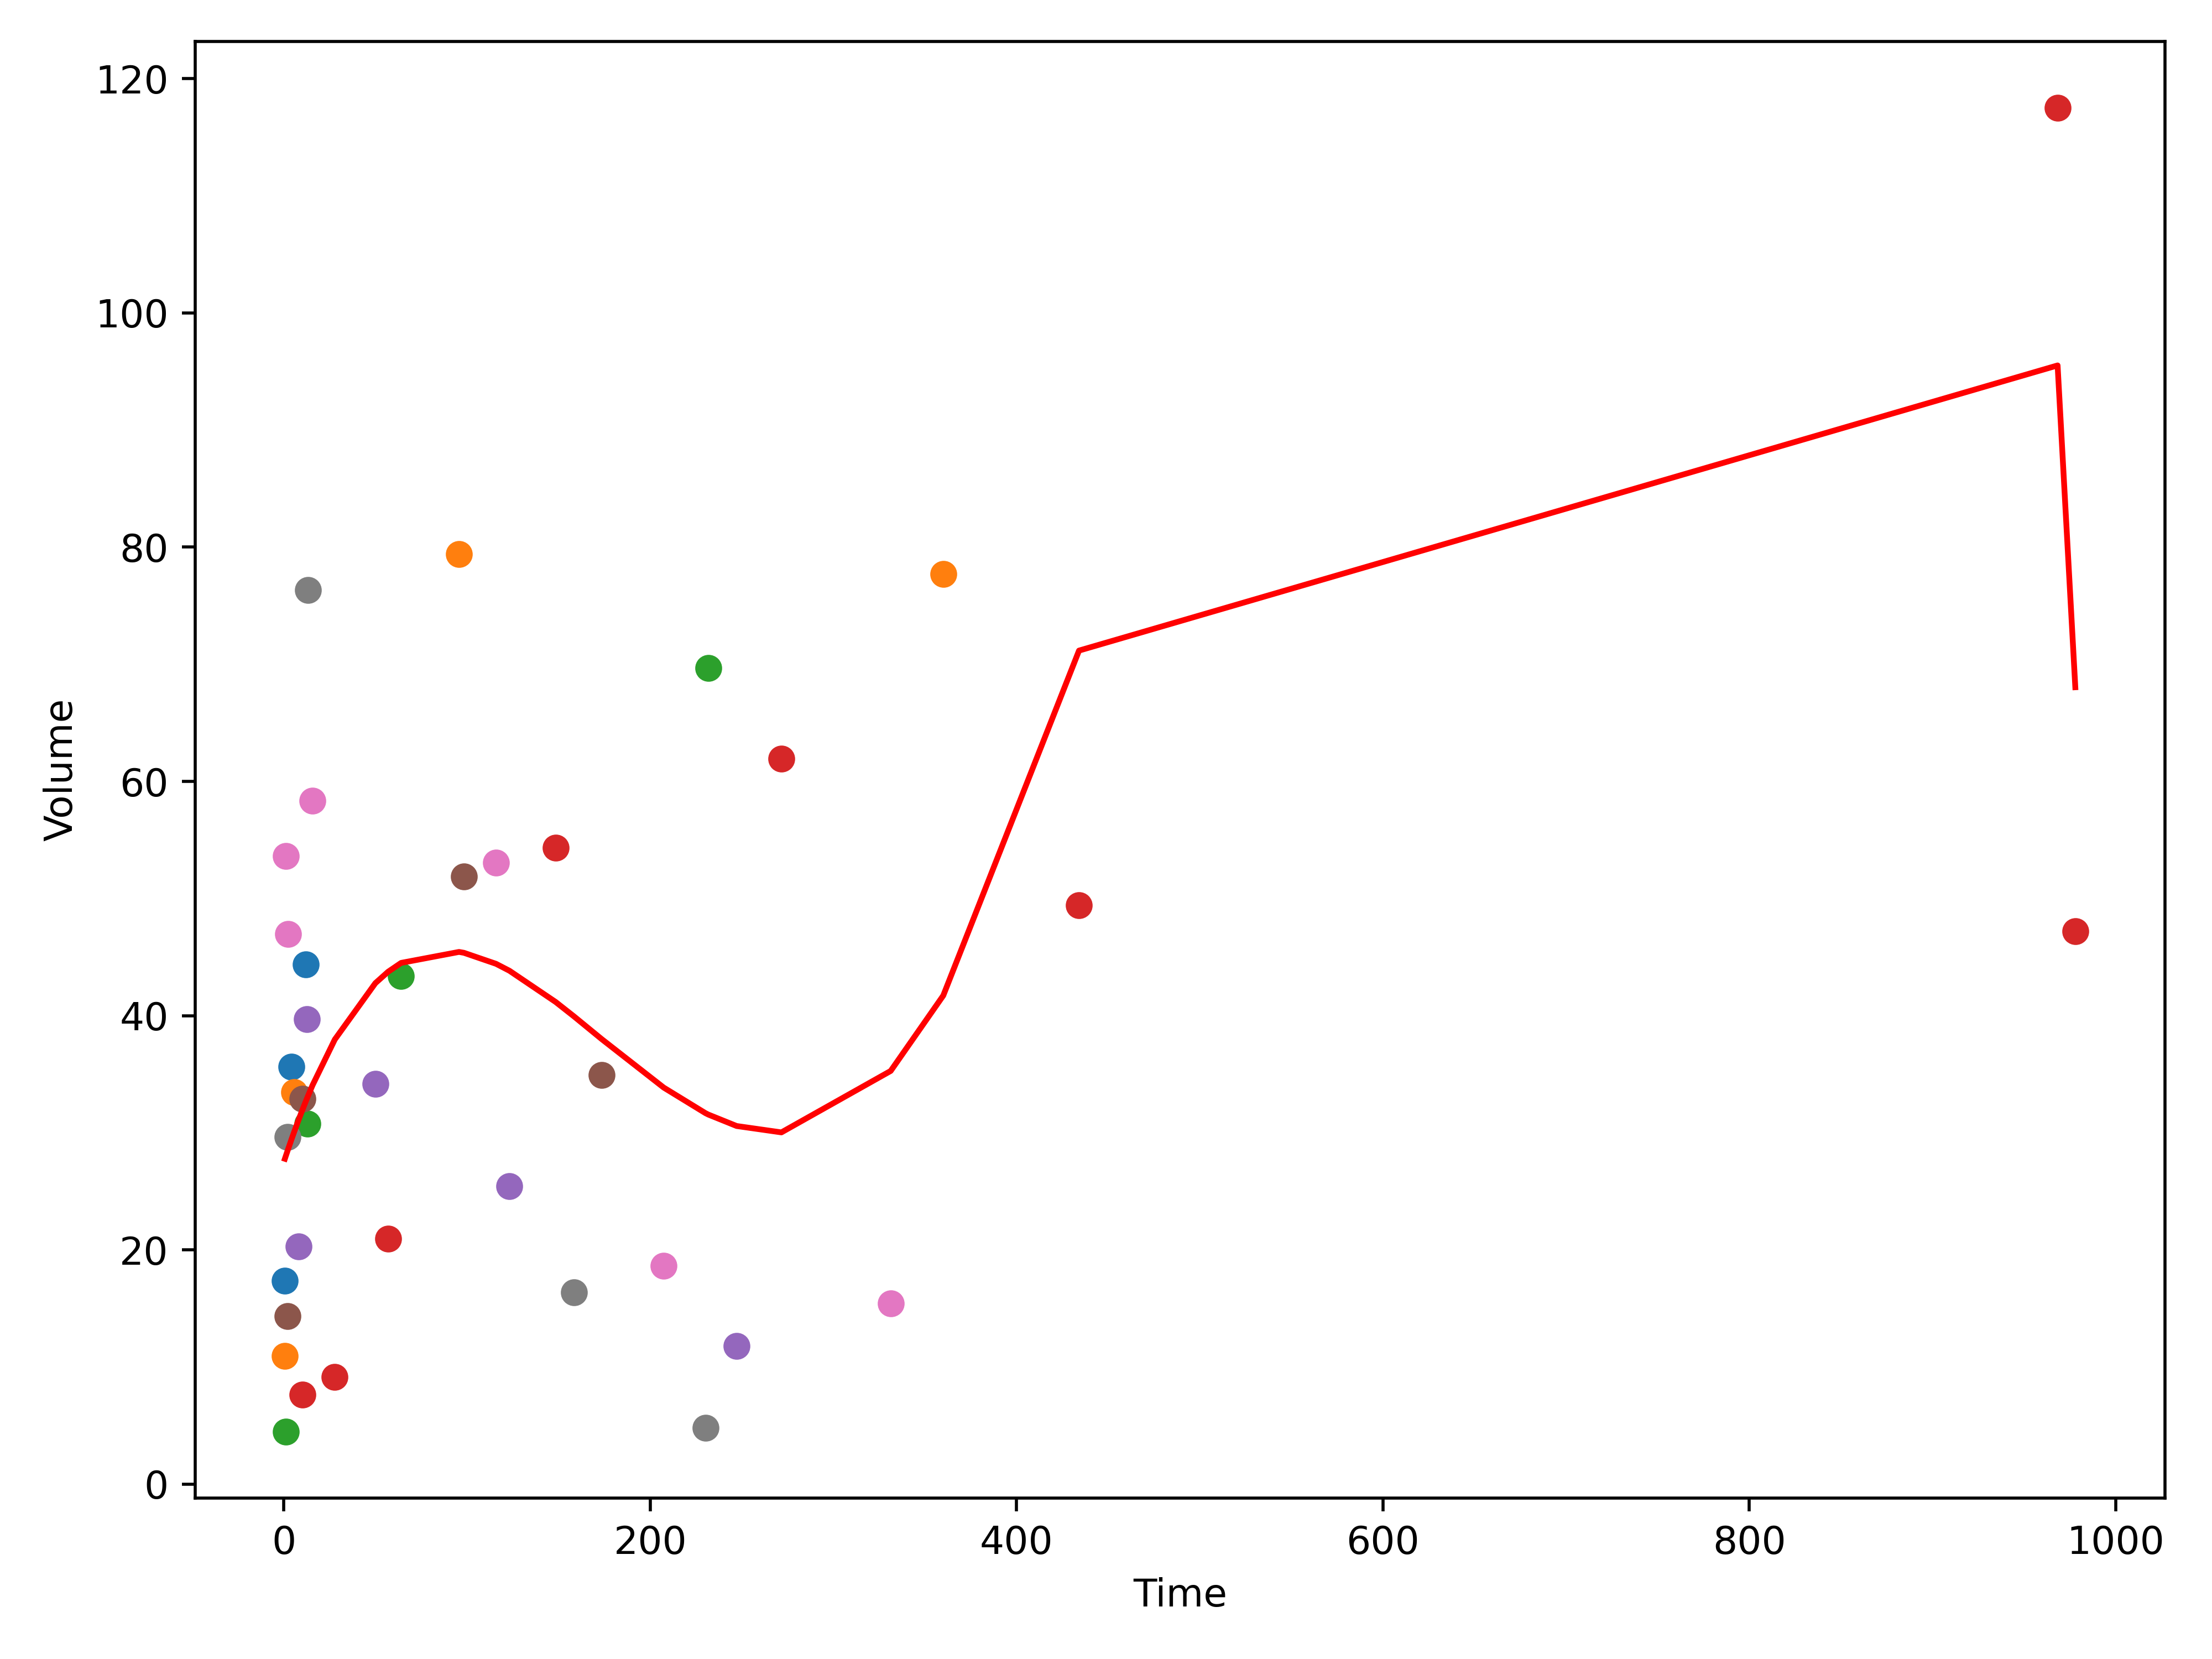
\includegraphics[width=0.33\textwidth]{class24次多项式回归散点图.png}}
					\caption{分亚组拟合曲线}
					\label{fig:12}
				\end{figure}
				
				\textbf{三、治疗方法与水肿体积进展关系}
				
				依据分析中的方法,我们首先将治疗方法与水肿体积进展构建训练数据,随后分别对数据\textbf{计算灰度关联系数、Spearman相关系数、Kendall相关系数、随机森林重要性得分}等。
				
				灰度关联系数是一种用于衡量因素间关联程度的方法。它的基本思想是通过计算主因子序列和每个行为因子序列之间的灰色关联度,来判断因子之间关系的强度、大小和顺序。如果两个因素变化的趋势具有一致性,即同步变化程度较高,那么我们可以认为这两者的关联程度较高;反之,则较低1。灰度关联系数公式如下:
				\[
				y(x0(k),xi(k))=\frac{\mathrm{minmin}|x0(k)-xi(k)|+\rho\mathrm{maxmax}|x0(k)-xi(k)|}{|x0(k)-xi(k)|+\rho\mathrm{maxmax}|x0(k)-xi(k)|}
				\]
				
				斯皮尔曼等级相关系数,简称斯皮尔曼相关系数,是由查尔斯·斯皮尔曼于1904年提出的,用于衡量两个变量之间的相关性。它是一种非参数统计方法,适用于任何类型的数据,包括有序、等级或连续数据。斯皮尔曼相关系数通过将两个变量的观察值转换为等级,然后计算等级之间的相关性来衡量变量之间的关系。斯皮尔曼相关系数计算公式如下:
				\[
				\rho=1-\frac{6\sum d_{i}^{2}}{n(n^{2}-1)}
				\]
				
				肯德尔系数,也称为肯德尔秩相关系数,是一种用来测量两个随机变量相关性的统计值。它的目标对象是有序的类别变量,比如名次、年龄段、肥胖等级等。肯德尔系数的取值范围在-1到1之间,当$\tau$为1时,表示两个随机变量拥有一致的等级相关性;当$\tau$为-1时,表示两个随机变量拥有完全相反的等级相关性;当$\tau$为0时,表示两个随机变量是相互独立的。肯德尔系数计算公式如下:
				\[
				\tau=\frac{(\text{和谐的观察值对}-\text{不和谐的观察值对的数量})}{0.5\times n\times(n-1)}
				\]
				
				随机森林的基本原理如章节\ref{lilun}所述,随机森林重要性得分则是一种衡量特征在随机森林模型中的重要程度的方法。这种评估方法的基本思想是看每个特征在随机森林中的每颗树上做了多大的贡献。
				
				基于上述原理,我们分别计算了每个治疗方法与水肿体积进展之间的相关性系数,如表所示;
				
				\begin{table}[H]
					\centering
					\begin{tabular}{|c|c|c|c|c|}
						\hline
						\rowcolor{green!30} 治疗方法 & 灰度关联系数 & Spearman系数 & Kendall系数 & 随机森林重要性得分 \\ \hline
						\rowcolor{green!5}脑室引流 & 0.235915 & 0.09813 & 0.080445 & 0.080644 \\ \hline
						\rowcolor{white!5}止血治疗 & -0.007515 & 0.11758 & 0.09639 & 0.1990965 \\ \hline
						\rowcolor{green!5}降颅压治疗 & 0.144045 & 0.230165 & 0.188685 & 0.180942 \\ \hline
						\rowcolor{white!5}降压治疗 & 0.120355 & 0.221375 & 0.18148 & 0.139967  \\ \hline
						\rowcolor{green!5}镇静、镇痛治疗 & 0.09117 & 0.12949 & 0.106155 & 0.15616 \\ \hline
						\rowcolor{white!5}止吐护胃 & 0.02071 & 0.006835 & 0.0056 & 0.095942 \\ \hline
						\rowcolor{green!5}营养神经 & 0.069045 & 0.1518 & 0.124445 & 0.1472485 \\ \hline
					\end{tabular}
				\end{table}
				
				所以,我们根据分析结果的出来的结论如下:
				
				\begin{table}[H]
					\centering
					\rowcolors{1}{blue!8}{white}
					\begin{tabularx}{\textwidth}{|X|}
						\hline
						\begin{enumerate}
							\item 灰度关联分析:
							
							脑室引流与灰度关联系数呈正相关,脑室引流治疗可能导致灰度值增加。
							
							止血治疗与灰度关联系数接近零,止血治疗对灰度值影响较小。
							
							降颅压治疗与灰度关联系数呈正相关,降颅压治疗可能导致灰度值增加。
							
							降压治疗与灰度关联系数呈正相关,降压治疗可能导致灰度值增加。
							
							镇静、镇痛治疗与灰度关联系数呈正相关,镇静、镇痛治疗可能导致灰度值增加。
							
							止吐护胃与灰度关联系数呈正相关,止吐护胃治疗可能导致灰度值增加。
							
							营养神经与灰度关联系数呈正相关,营养神经治疗可能导致灰度值增加。
							
							\item 斯皮尔曼相关性分析(按相关系数从大到小排序):
							
							降颅压治疗:0.230165;降压治疗:0.221375;营养神经:0.1518;镇静、镇痛治疗:0.12949;止血治疗:0.11758;脑室引流:0.09813;止吐护胃:0.006835
							
							所有治疗方法都呈正相关,降颅压治疗具有最强的正相关性,而止吐护胃的相关性最低。所有方法都对水肿体积进展产生积极影响。
							
							\item Kendall秩相关性分析(按相关系数从大到小排序):
							
							降颅压治疗:0.188685;降压治疗:0.18148;营养神经:0.124445;镇静、镇痛治疗:0.106155;止血治疗:0.09639;脑室引流:0.080445;止吐护胃:0.0056
							
							所有治疗方法都呈正相关,降颅压治疗和降压治疗的相关性较高,而止吐护胃的相关性最低。
							
							\item 随机森林重要性分析(按重要性得分从大到小排序):
							
							止血治疗:0.1990965;降颅压治疗:0.180942;镇静、镇痛治疗:0.15616;营养神经:0.1472485;降压治疗:0.139967;止吐护胃:0.095942;脑室引流:0.080644
							
							根据随机森林模型的重要性得分,止血治疗具有最高的重要性,其次是降颅压治疗和镇静、镇痛治疗。脑室引流的重要性相对较低。需要注意的是,这些分析结果不能简单用来确定因果关系或绝对的治疗效果,仍需要进一步的临床验证和考虑其他因素。
							
						\end{enumerate}\\
						\hline
					\end{tabularx}
				\end{table}
				
				\textbf{四、血肿水肿治疗方法三者关系}
				
				依据分析,我们将血肿体积、水肿体积、治疗方法三方数据整合,生成新的训练数据表,随后我们对三个特征进行\textbf{单因素方差分析、多因素方差分析、热力图分析}等。
				
				通过上述分析所获得的分析结果如下:
				
				\begin{table}[H]
					\centering
					\label{tab:11}
					\caption{单因素方差分析结果}
					\begin{tabular}{|c|c|c|c|c|c|c|c|}
						\hline
						\rowcolor{green!35} \multicolumn{4}{|c|}{血肿} & \multicolumn{4}{c|}{水肿}\\ \hline
						\rowcolor{green!25} ID & F & P & 显著关系 & ID & F & P & 显著关系 \\ \hline
						\rowcolor{green!5}脑室引流 & 10.0546 & 0.0019 & 非常显著 & 脑室引流 & 11.8015 & 0.0008 & 非常显著 \\ \hline
						\rowcolor{white!5}止血治疗 & 0.0415 & 0.8388 & 不显著 & 止血治疗 & 0.1037 & 0.7479 & 不显著 \\ \hline
						\rowcolor{green!5}降颅压治疗 & 3.9367 & 0.0494 & 不显著 & 降颅压治疗 & 1.3418 & 0.2488 & 不显著 \\ \hline
						\rowcolor{white!5}降压治疗 & 0.9658 & 0.3276 & 不显著 & 降压治疗 & 0.7682 & 0.3824 & 不显著 \\ \hline
						\rowcolor{green!5}镇静镇痛 & 0.1531 & 0.6962 & 不显著 & 镇静镇痛 & 2.0150 & 0.1582 & 不显著 \\ \hline
						\rowcolor{white!5}止吐护胃 & 0.9631 & 0.3282 & 不显著 & 止吐护胃 & 0.1903 & 0.6634 & 不显著 \\ \hline
						\rowcolor{green!5}营养神经 & 0.5716 & 0.4510 & 不显著 & 营养神经 & 1.5825 & 0.2107 & 不显著 \\ \hline
					\end{tabular}
				\end{table}
				
				\begin{table}[H]
					\centering
					\caption{多因素方差分析结果(水肿与治疗方法)}
					\begin{tabular}{|c|c|c|c|c|c|c|}
						\hline
						\rowcolor{green!30}\textbf{水肿} & df & sum\_sq & mean\_sq & F & PR(>F) & 显著水平 \\ \hline
						\rowcolor{green!5}脑室引流 & 1 & 2274423254 & 2274423254 & 11.88736337 & 0.000780087 & 有影响 \\ \hline
						\rowcolor{white!5}止血治疗 & 1 & 2342260.348 & 2342260.348 & 0.012241917 & 0.91208413 & 无影响 \\ \hline
						\rowcolor{green!5}降压治疗 & 1 & 66995698.07 & 66995698.07 & 0.350155674 & 0.555138191 & 无影响 \\ \hline
						\rowcolor{white!5}降颅压治疗 & 1 & 220738046.6 & 220738046.6 & 1.153696158 & 0.284931819 & 无影响 \\ \hline
						\rowcolor{green!5}止吐护胃 & 1 & 10971807.4 & 10971807.4 & 0.057344587 & 0.81115179 & 无影响 \\ \hline
						\rowcolor{white!5}营养神经 & 1 & 192283012.6 & 192283012.6 & 1.004974794 & 0.318126942 & 无影响 \\ \hline
						\rowcolor{green!5}镇静治疗 & 1 & 830021941.2 & 830021941.2 & 4.338142606 & 0.03939155 & 有影响 \\ \hline
					\end{tabular}
				\end{table}
				
				\begin{table}[H]
					\centering
					\caption{多因素方差分析结果(血肿与治疗方法)}
					\begin{tabular}{|c|c|c|c|c|c|c|}
						\hline
						\rowcolor{green!30}\textbf{血肿} & df & sum\_sq & mean\_sq & F & PR(>F) & 显著水平 \\ \hline
						\rowcolor{green!5}脑室引流 & 1 & 7835648316 & 7835648316 & 10.03973981 & 0.001943676 & 有影响 \\ \hline
						\rowcolor{white!5}止血治疗 & 1 & 308113857.3 & 308113857.3 & 0.394783282 & 0.530989802 & 无影响 \\ \hline
						\rowcolor{green!5}降压治疗 & 1 & 332895792 & 332895792 & 0.426536134 & 0.514942872 & 无影响 \\ \hline
						\rowcolor{white!5}降颅压治疗 & 1 & 2462670419 & 2462670419 & 3.155395604 & 0.07821054 & 无影响 \\ \hline
						\rowcolor{green!5}止吐护胃 & 1 & 475146928.1 & 475146928.1 & 0.608801128 & 0.436775914 & 无影响 \\ \hline
						\rowcolor{white!5}营养神经 & 1 & 71447158.64 & 71447158.64 & 0.091544548 & 0.762746517 & 无影响 \\ \hline
						\rowcolor{green!5}镇静治疗 & 1 & 887029961.3 & 887029961.3 & 1.136542843 & 0.288524277 & 无影响 \\ \hline
					\end{tabular}
				\end{table}
				
					\begin{figure}[H]
					\centering
					\caption{三者之间相关热力图}
					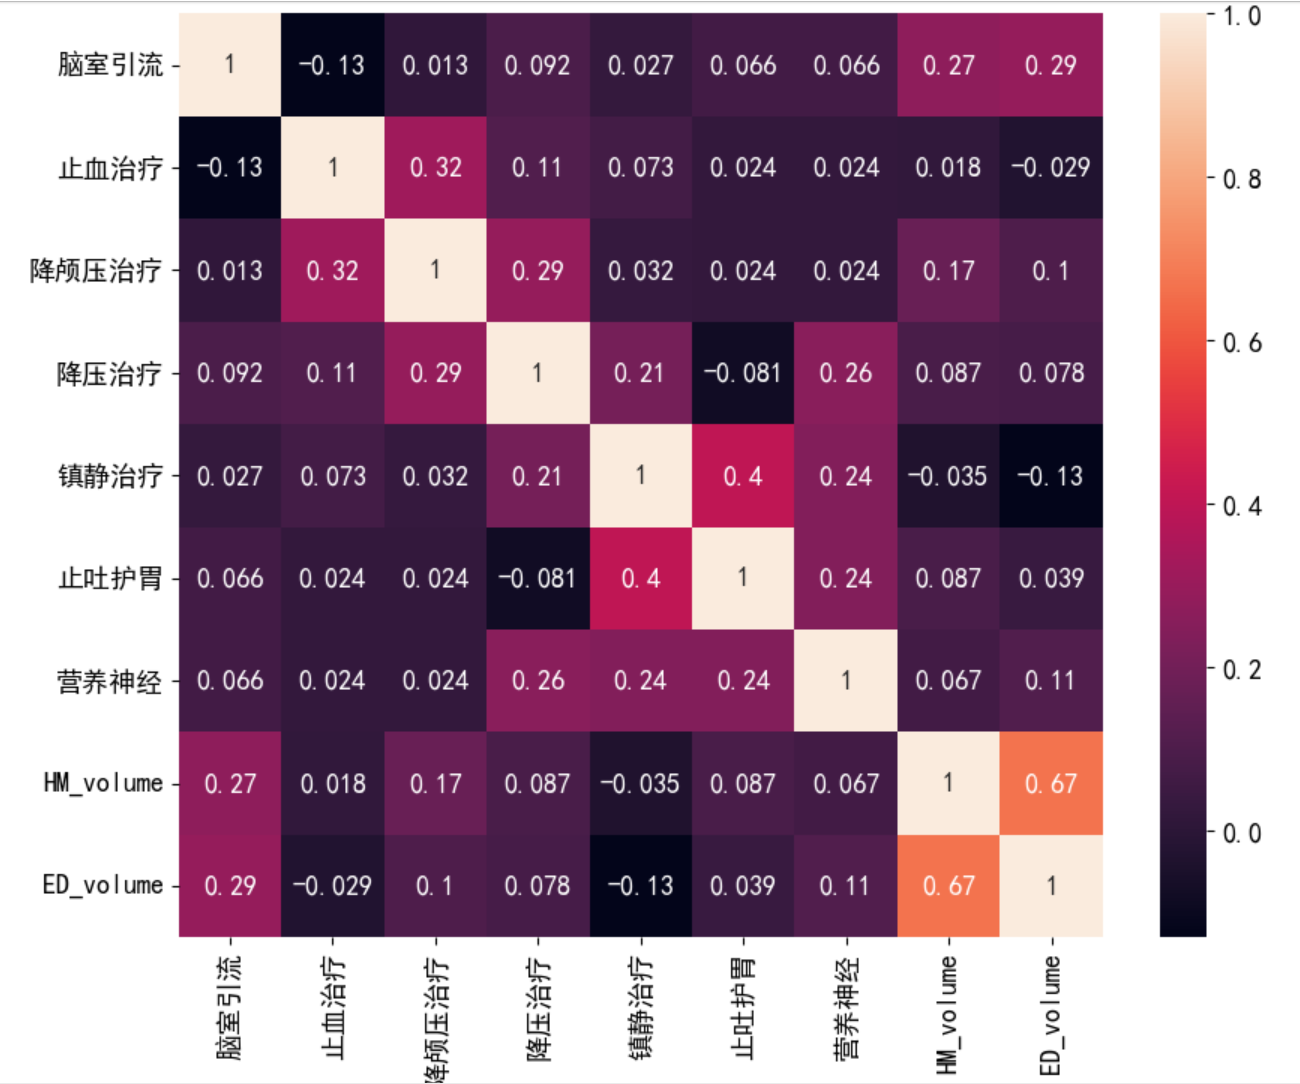
\includegraphics[width=.70\textwidth]{2d热力图.png}
					\label{fig:13}
				\end{figure}
				
				结合对上述结果的总结,我们能够得到如下分析:
				
				\begin{table}[H]
					\centering
					\rowcolors{1}{blue!8}{white}
					\begin{tabularx}{\textwidth}{|X|}
						\hline
						\begin{enumerate}
							\item 单因素变量(ANOVA)分析:
							
							水肿:
							脑室引流与水肿之间显著性水平较低,二者可能存在显著影响,其余方案与水肿之间显著性水平较高,可能不存在显著影响。
							
							血肿:
							脑室引流与血肿之间显著性水平较低,二者可能存在显著影响,其余方案与血肿之间显著性水平较高,可能不存在显著影响。
							
							\item 多因素变量(MANOVA)分析:
							
							治疗方案对水肿的影响:
							脑室引流与水肿之间显著性水平较低,二者可能存在显著影响,镇静、镇痛治疗与水肿之间显著性水平较低,二者可能存在显著影响,其余方案与水肿之间显著性水平较高,可能不存在显著影响。
							
							各种治疗方案对血肿的影响:
							脑室引流与水肿之间显著性水平较低,二者可能存在显著影响,其余方案与水肿之间显著性水平较高,可能不存在显著影响。
							\item 热力图分析:
							
							通过观察热力图发现:血肿体积和水肿体积之间具有较强的相关性。
							
						\end{enumerate}\\
						\hline
					\end{tabularx}
				\end{table}
		
		\subsection{【问题三】患者预后预测及关键因素探索}
			\subsubsection{问题分析3a:患者90天mRS预测}
				该问要求我们根据100个患者(sub001至sub100)个人史、疾病史、发病相关及首次影像结果构建预测模型,预测全部患者90天mRS评分,限制条件为训练数据仅可使用首次影像结果而不能使用后续影像检查结果,mRS分为6级,我们需要先按照限制要求拼接出训练所需的数据集,并完成数据的处理和转换。
				
				该题为一个多分类预测问题,我们仍然可以使用章节\ref{lilun}中的\textbf{LightGBM、XGBoost、随机森林、MLP},同时我们还可以加上\textbf{KNN聚类}方法,通过多个方法进行投票,选出得票数量高的结果作为最终的结果。并完成对所有患者90天mRS评分的多分类预测。
				
			\subsubsection{问题分析3b:增强数据的患者90天mRS预测}
				该问为前一问基础上,增加后续所有随访检测结果,扩大数据量的前提情况下,再一次对患者的90天mRS评分进行多分类预测。我们需要重新凭借训练所需数据集,并且处理好部分患者因无后续随访而导致随访结果缺失的情况。
			
				对于该问的解答,我们希望在拥有更多数据量的情况下,同时\textbf{对前一问的解决算法进行网格搜索,优化模型参数},在数据量和模型性能双双提升的效果过,整体模型投票效果增强,最终获得一个更好预测结果。
			
			\subsubsection{问题分析3c:患者多因素关联关系分析与建议}
				该问要求我们分析出血性脑卒中患者的预后(90天mRS)和个人史、疾病史、治疗方法及影像特征(包括血肿/水肿体积、血肿/水肿位置、信号强度特征、形状特征)等关联关系,为临床相关决策提出建议。
				
				首先我们需要对各个特征变量本身进行特征工程分析,对特征进行\textbf{频率频数以及分布分析},同时也要对特征之间进行分布关系关联对比,需要输出一些分布结果。
				
				与问题二中几个分析类似,我们考虑对多因素进行\textbf{热力图分析、相关系数分析以及通过随机森林对多因素进行重要性排序},通过对分析结果进行解读,我们就可以得到多因素之间的关联关系。
				
				问题三整体流程图如图\ref{fig:17}所示:
				
				\begin{figure}[H]
					\centering
					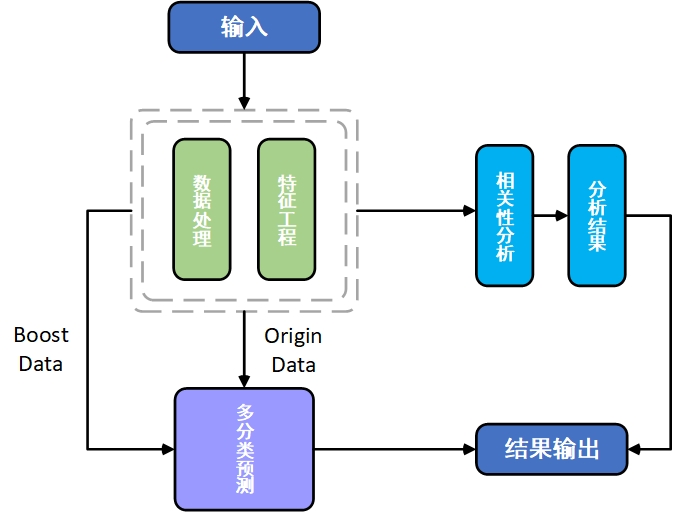
\includegraphics[width=.60\textwidth]{问题三流程图.jpg}
					\caption{问题三流程图}
					\label{fig:17}
				\end{figure}
			
			\subsubsection{模型建立与求解}
				\textbf{一、患者90天mRS预测}

				按照分析,我们获得了限制要求条件下的训练数据,我们将训练数据分别输入到五个模型中进行预测,五个模型的预测结果评估指标如下表所示:
				
				\begin{table}[H]
					\centering
					\caption{3a模型训练结果对比}
					\label{tab:13}
					\setlength{\tabcolsep}{7mm}
					\begin{tabular}{|c|c|c|c|c|}
						\hline
						\rowcolor{green!30} Model & Accuracy & Precision &Recall & F1 \\ \hline
						\rowcolor{green!5}LightGBM & 0.2  & \textbf{0.31428} & 0.17142& 0.1630\\ \hline
						\rowcolor{white!5}MLP & 0.15  & 0.16326
						& 0.12380 & 0.1265\\ \hline
						\rowcolor{green!5}RF & 0.2  & 0.15476
						& 0.17142 & 0.1403\\ \hline
						\rowcolor{white!5}KNN & \textbf{0.3}  & 0.18367
						& \textbf{0.24761} & \textbf{0.19202}\\ \hline
						\rowcolor{green!5}XGBoost& 0.15 & 0.17857  & 0.12380 & 0.0995 \\ \hline
					\end{tabular}
				\end{table}
				
				分析表我们可以发现,KNN模型在这个多分类预测中性能要稍好于其他模型,其中效果不理想的随机森林RF模型在训练集和测试集上学习曲线对比如下,可以看到明显发生了过拟合现象:
				
			
				\begin{figure}[H]
				\centering
				\caption{随机森林学习曲线}
				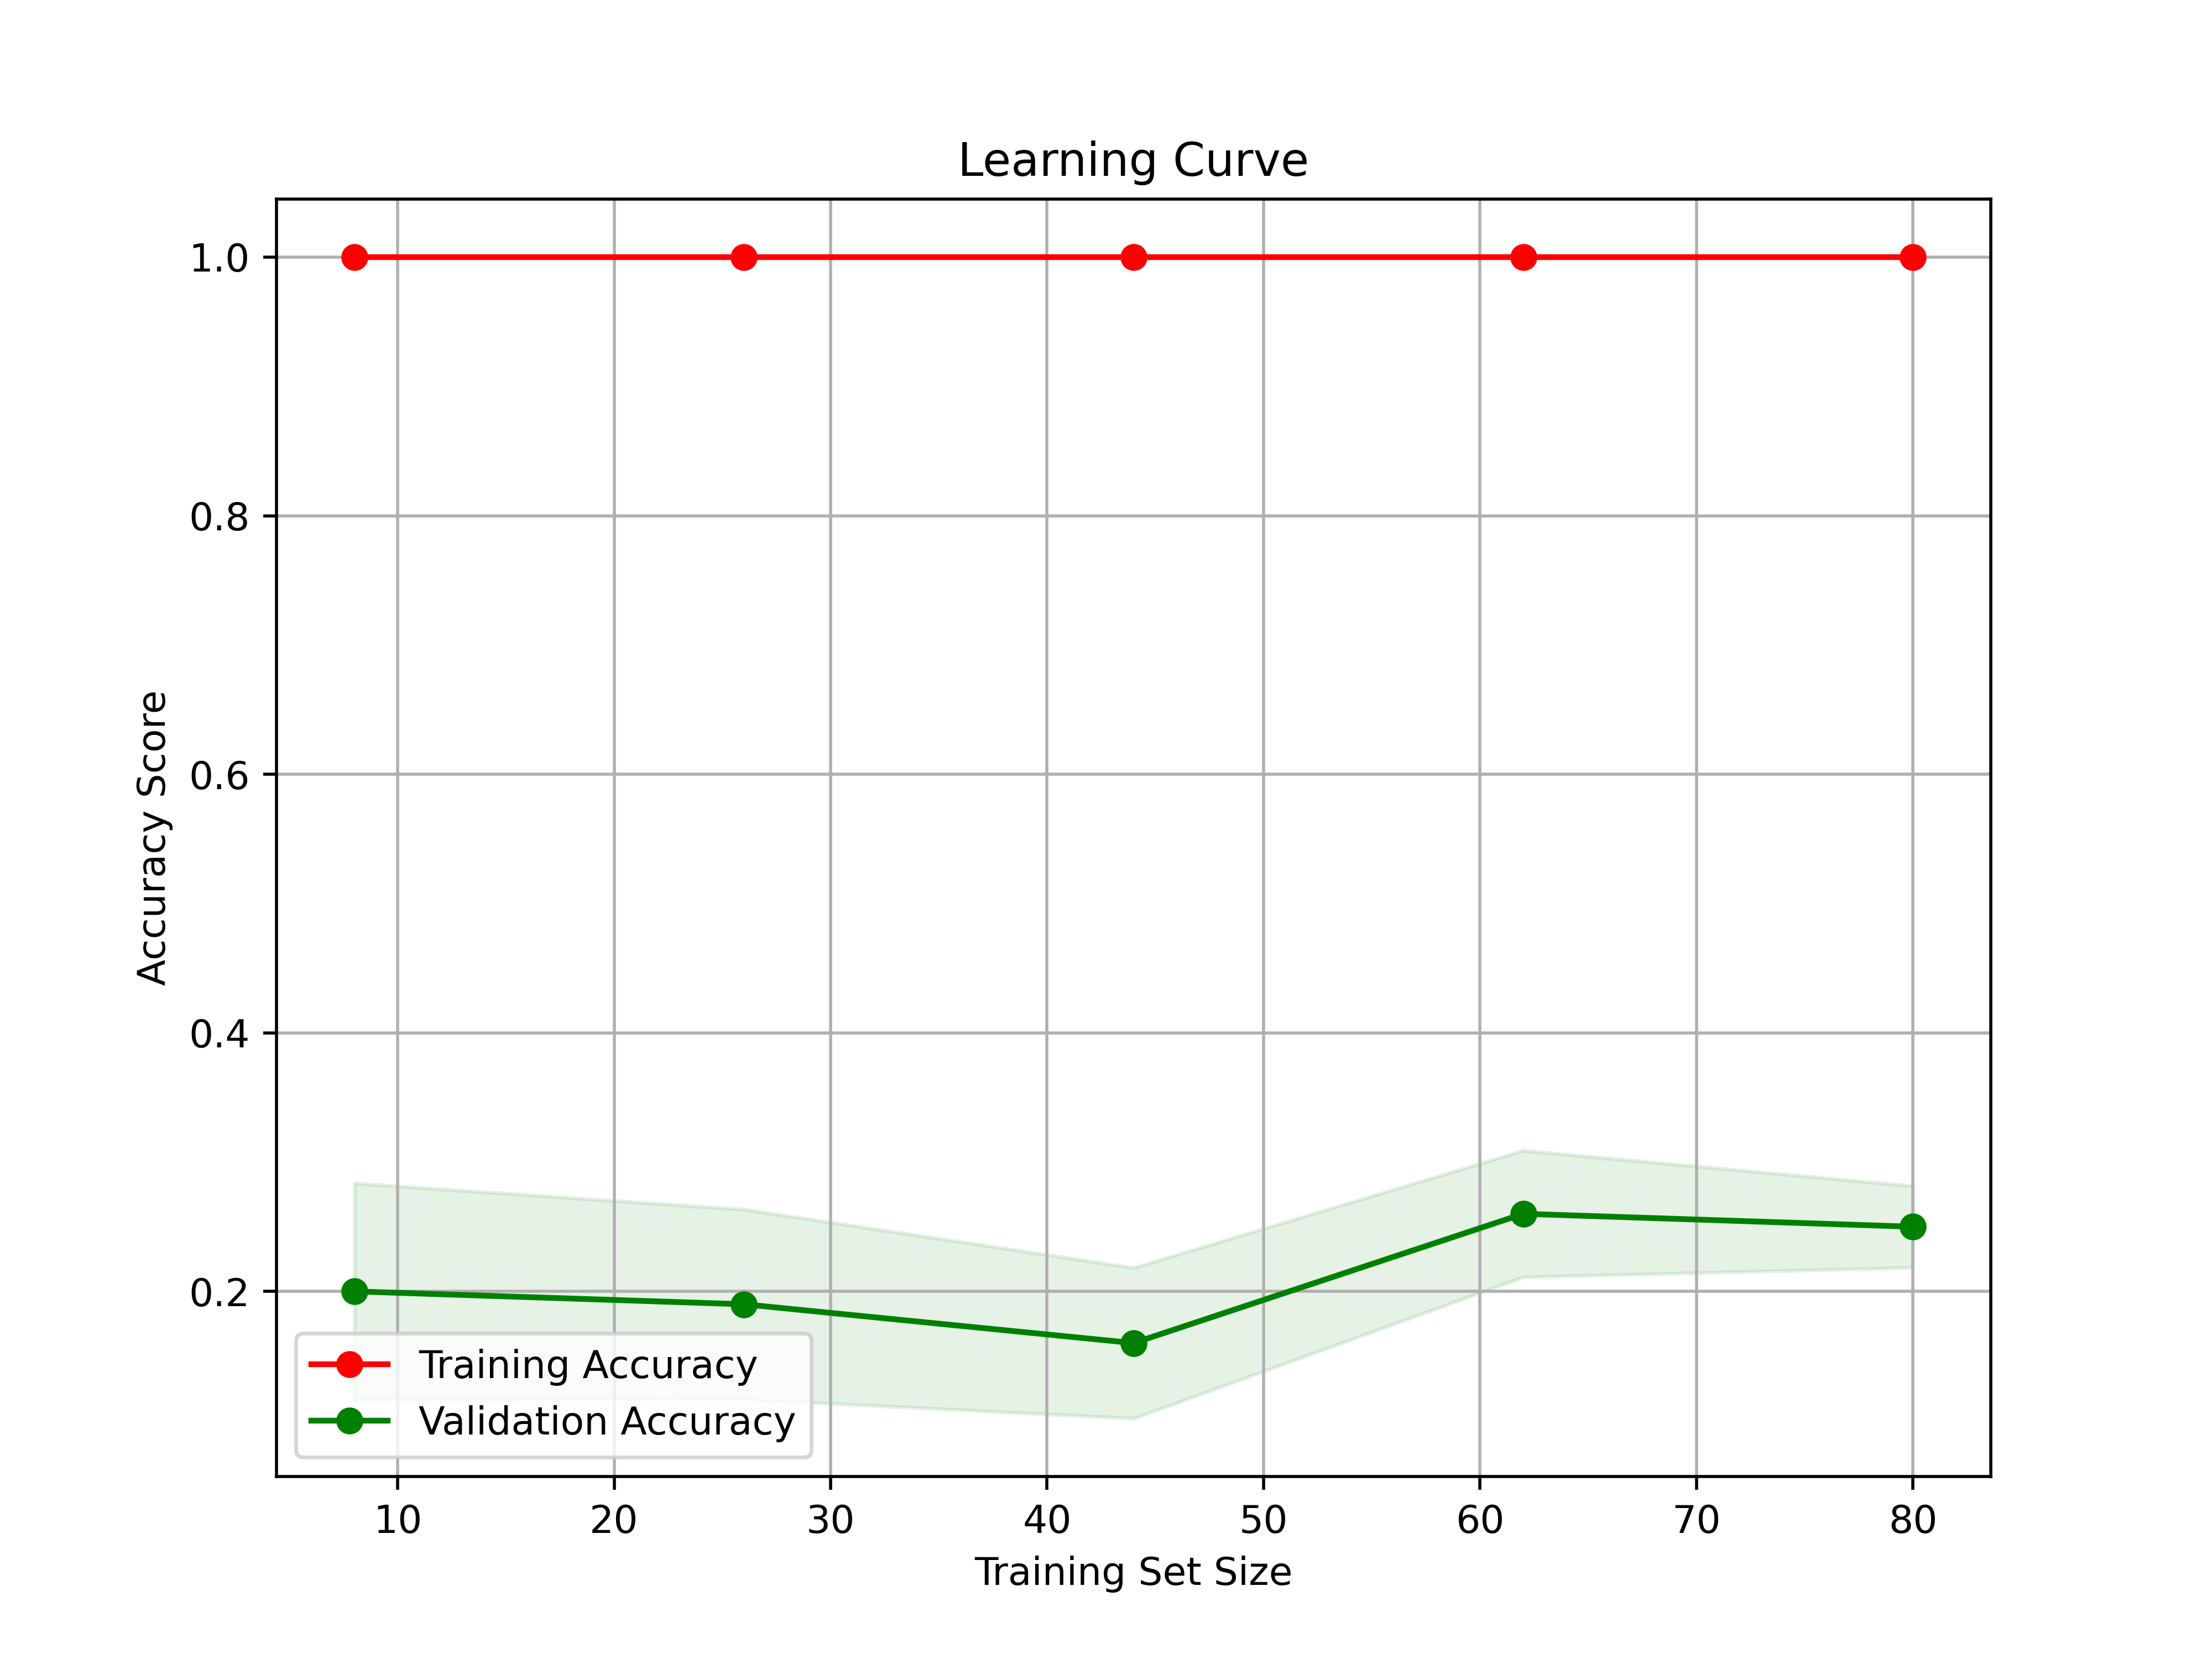
\includegraphics[width=.65\textwidth]{RF学习曲线.png}
				\label{fig:15}
				\end{figure}
				
				经过多模型投票预测结果,我们能得到如下答案:
				
				\begin{table}[H]
					\centering
					\label{tab:14}
					\caption{患者90天mRS预测结果(部分数据)}
					\setlength{\tabcolsep}{17mm}
					\begin{tabular}{|c|c|}
						\hline
						\rowcolor{blue!25} ID & mRS \\ \hline
						\rowcolor{blue!5}sub001 & 4 \\ \hline
						\rowcolor{white!5}sub003 & 3\\ \hline
						\rowcolor{blue!5}sub008 & 3 \\ \hline
						\rowcolor{white!5}sub011 & 1  \\ \hline
						\rowcolor{blue!5}sub002 & 0  \\ \hline
					\end{tabular}
				\end{table}
				
				\textbf{二、增强数据的患者90天mRS预测}
				
				如前文分析所述,我们通过拼接数据表,发现有大量空缺值需要处理,空缺值基本位于患者后续随访次数导致的随访记录的缺失,这将导致特征的维度发生变化,通常有两种方式解决这个问题:\textbf{1、做特征转换,将多次随访数据转换为纵向样本方向的特征,相当于数据增广;2、将多次随访数据进行特征提取,整合成一个或多个定量特征}。
				
				我们采取第二种方式对数据进行处理,生成了新的训练数据表,并且我们重新对前一问模型全部进行了网格搜索,迭代优化了模型的参数,并且训练过程中采用\textbf{交叉验证}的方式进行数据集划分,最终得到的各模型评估指标结果如下:
				
				\begin{table}[H]
					\centering
					\caption{3b优化后模型训练结果对比}
					\label{tab:15}
					\setlength{\tabcolsep}{7mm}
					\begin{tabular}{|c|c|c|c|c|}
						\hline
						\rowcolor{green!30} Model & Accuracy & Precision &Recall & F1 \\ \hline
						\rowcolor{green!5}LightGBM & 0.35  & \textbf{0.41428} & 0.16142 & 0.1826\\ \hline
						\rowcolor{white!5}MLP & 0.3  & 0.30235
						& 0.26662 & 0.2352\\ \hline
						\rowcolor{green!5}RF & \textbf{0.4}  & 0.35883
						& \textbf{0.36194} & \textbf{0.3034}\\ \hline
						\rowcolor{white!5}KNN & 0.32  & 0.17931
						& 0.17262 & 0.1507\\ \hline
						\rowcolor{green!5}XGBoost& 0.15 & 0.17857  & 0.12380 & 0.0995 \\ \hline
					\end{tabular}
				\end{table}
				
				优化后,我们对所有患者的90天mRS重新进行了预测,同上一问中部分结果如下;
				
				\begin{table}[H]
					\centering
					\label{tab:16}
					\caption{优化后患者90天mRS预测结果(部分数据)}
					\setlength{\tabcolsep}{17mm}
					\begin{tabular}{|c|c|}
						\hline
						\rowcolor{blue!25} ID & mRS \\ \hline
						\rowcolor{blue!5}sub001 & 4 \\ \hline
						\rowcolor{white!5}\textbf{sub003} & \textbf{0}\\ \hline
						\rowcolor{blue!5}sub008 & 3 \\ \hline
						\rowcolor{white!5}sub011 & 1  \\ \hline
						\rowcolor{blue!5}sub002 & 0  \\ \hline
					\end{tabular}
				\end{table}
				
				其中,优化后的同一个算法学习曲线能够看到明显的性能提高,如下图所示:
				
				\begin{figure}[H]
					\centering
					\caption{随机森林学习曲线(优化后)}
					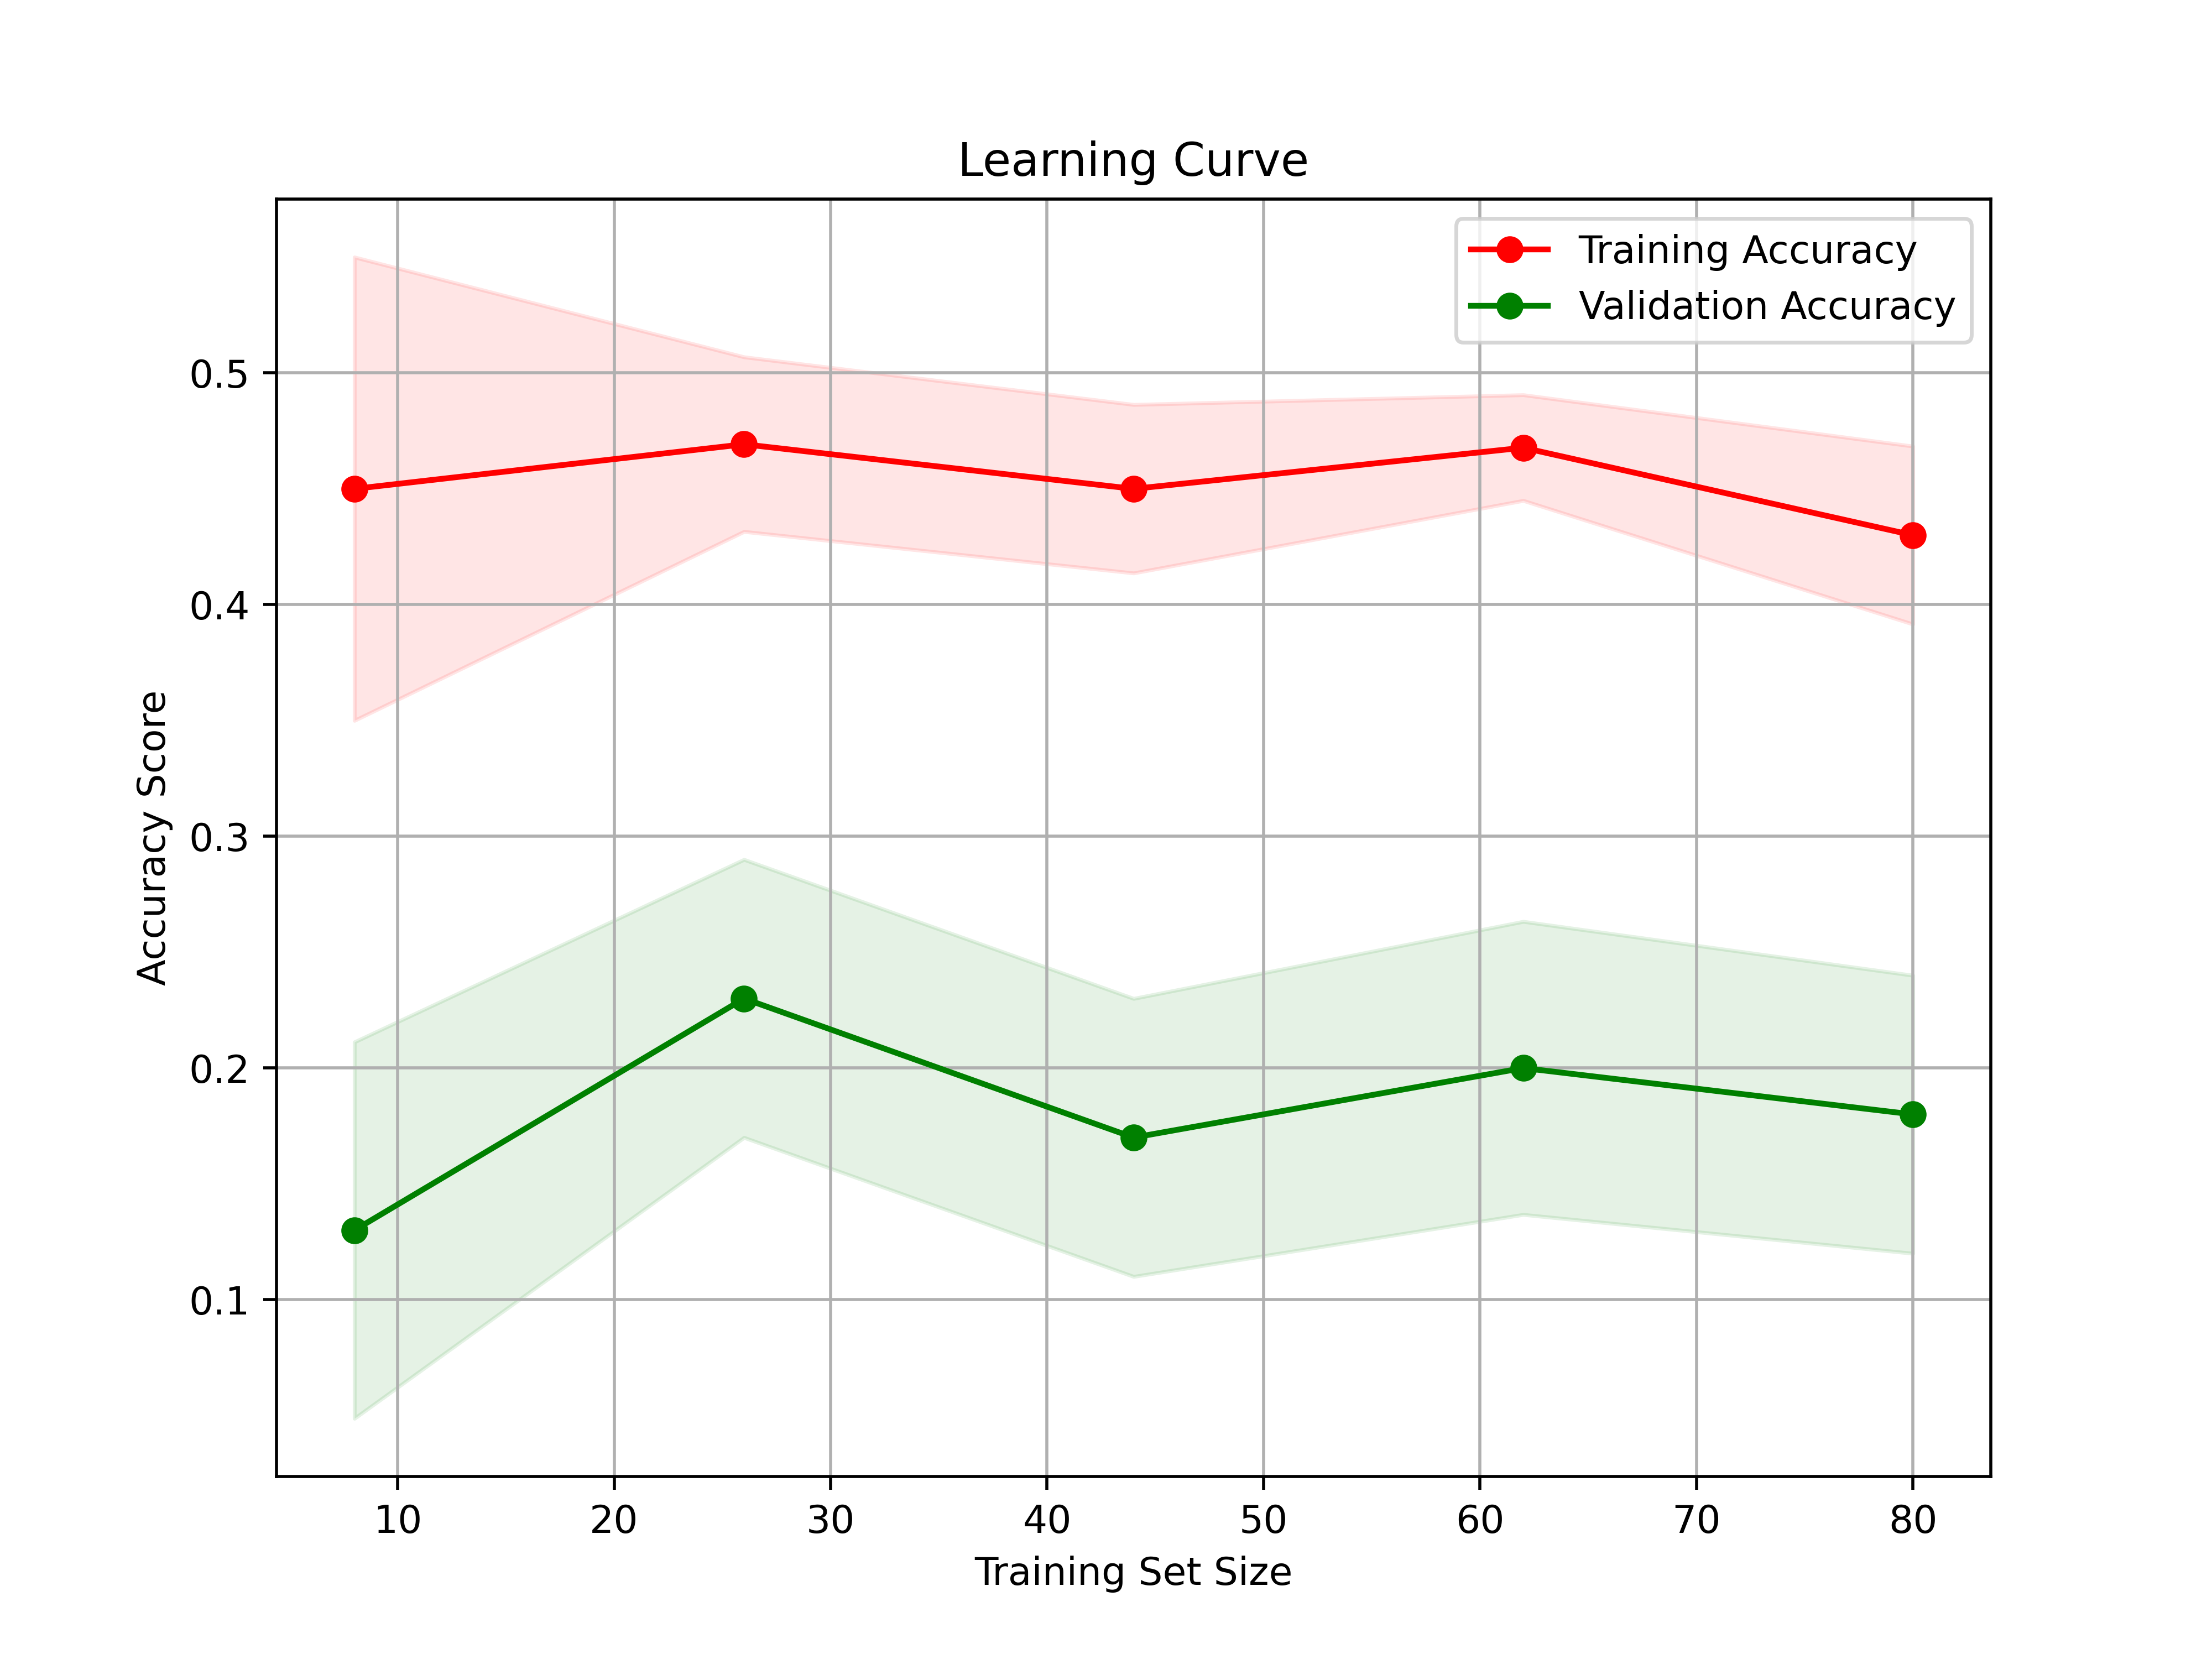
\includegraphics[width=.65\textwidth]{KNN学习曲线.png}
					\label{fig:14}
				\end{figure}
				
				\textbf{三、患者多因素关联关系及分析建议}
				
				首先,我们按照分析,先分别看看各个特征的相关统计学结果,比如说我们分析患者的疾病史,可以得到各项疾病在患者中的占比大小,占比如图所示:
				
				\begin{figure}[H]
					\centering
					\subfloat[房颤史]{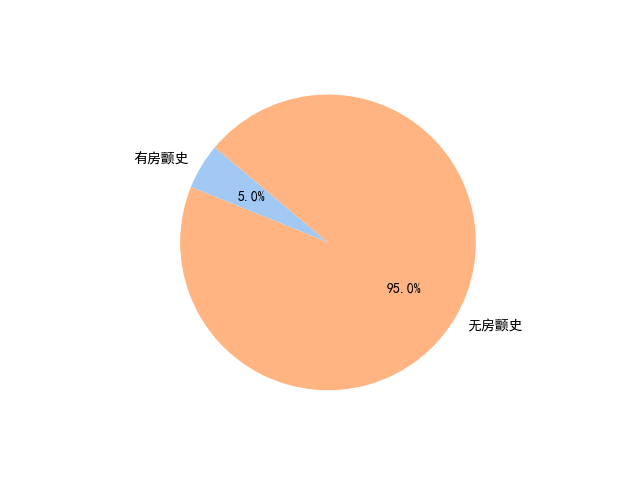
\includegraphics[width=0.30\textwidth]{房颤史占比图.png}}\qquad
					\subfloat[高血压史]{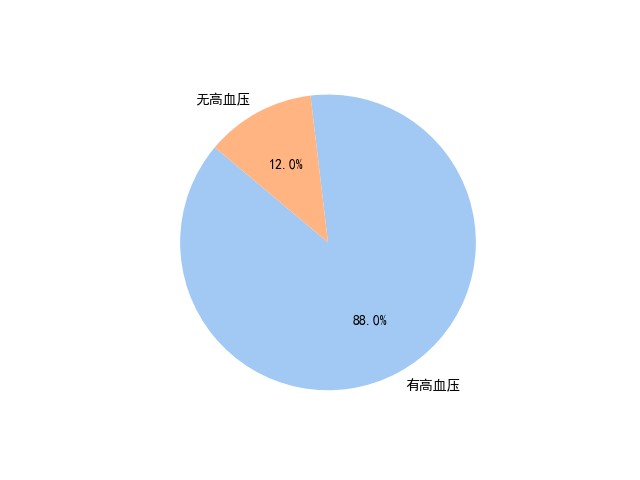
\includegraphics[width=0.30\textwidth]{高血压占比图.png}} \qquad
					\subfloat[糖尿病史]{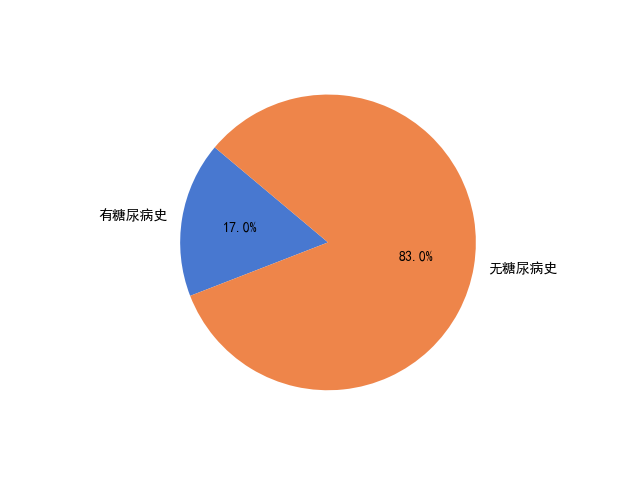
\includegraphics[width=0.30\textwidth]{糖尿病占比图.png}}\\
					\subfloat[吸烟史]{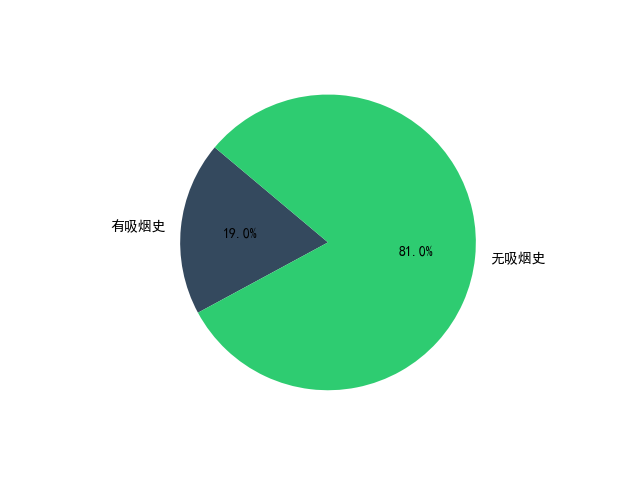
\includegraphics[width=0.30\textwidth]{吸烟史占比图.png}}\qquad
					\subfloat[饮酒史]{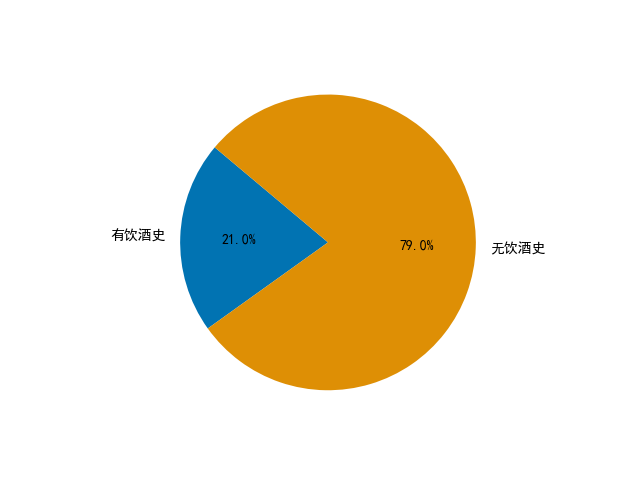
\includegraphics[width=0.30\textwidth]{饮酒史占比图.png}}\qquad
					\subfloat[冠心病史]{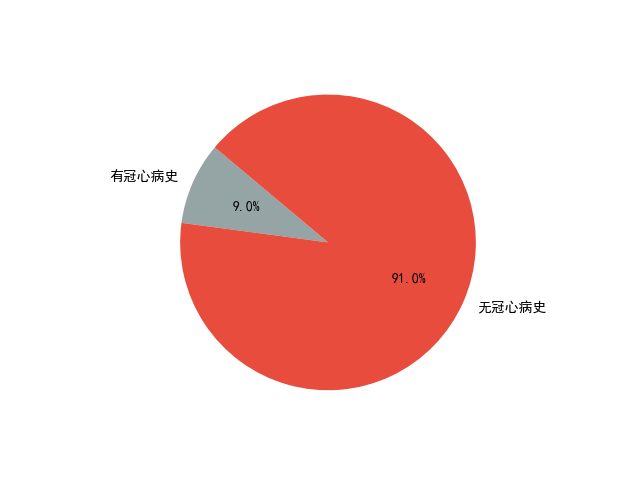
\includegraphics[width=0.30\textwidth]{有无冠心病史占比图.png}}\qquad
					\subfloat[卒中病史]{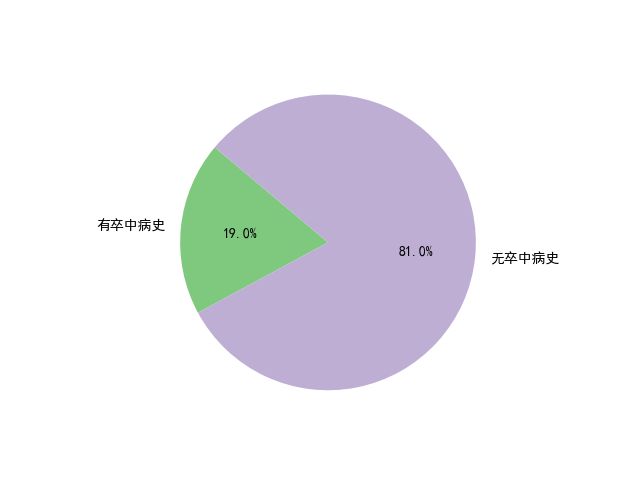
\includegraphics[width=0.30\textwidth]{有无卒中病史.png}}
					\caption{多方法拟合曲线对比}
				\end{figure}
				
				同时,我们也充分分析了变量与变量之间的相关特征,比如血肿体积、水肿体积与mRS之间的关系:
				
				\begin{figure}[H]
					\centering
					\subfloat[HM与mRS小提琴图]{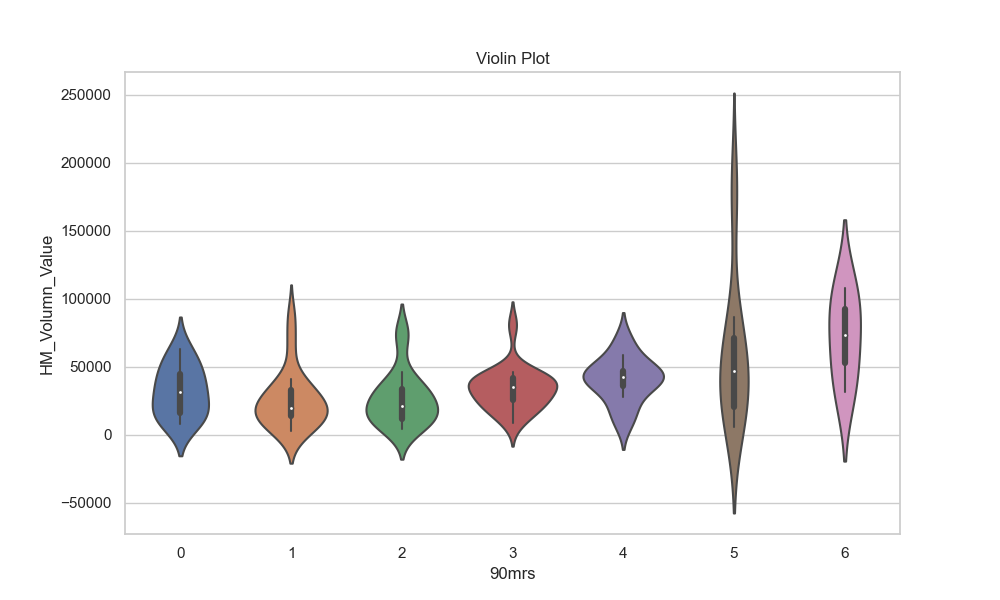
\includegraphics[width=0.45\textwidth]{HMVolume与target小提琴图.png}}\qquad
					\subfloat[ED与mRS小提琴图]{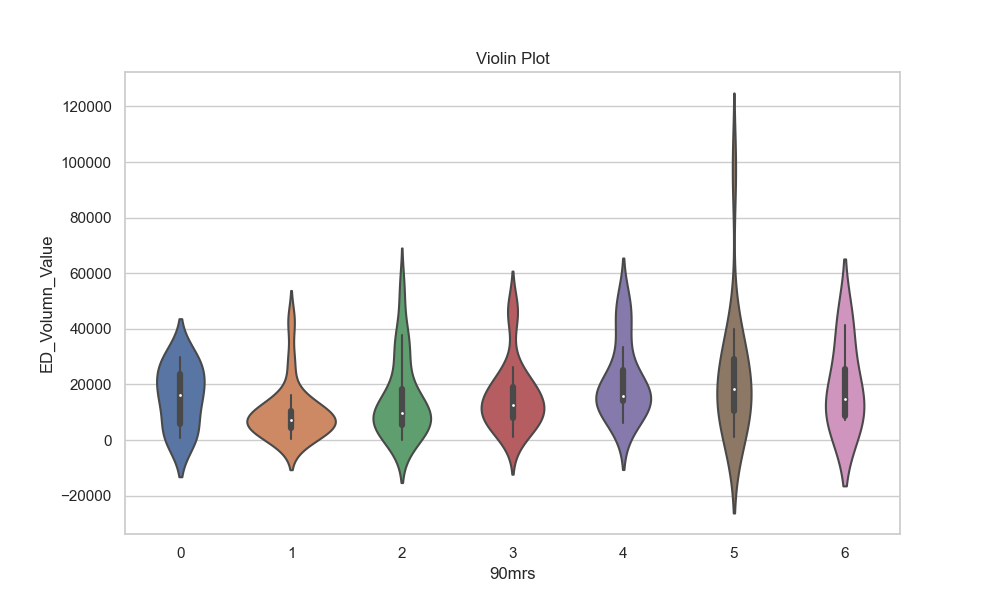
\includegraphics[width=0.45\textwidth]{EDVolume与target小提琴图.png}}
					\caption{多变量之间关系分析}
				\end{figure}
				
				分析完变量本身与变量间的统计学信息后,我们就可以将训练数据输入到相关性系数计算、热力图、以及随机森林特征重要性排序的算法中了。多因素间相关性热力图如下:
				
				\begin{figure}[H]
					\centering
					\caption{多因素之间相关性热力图}
					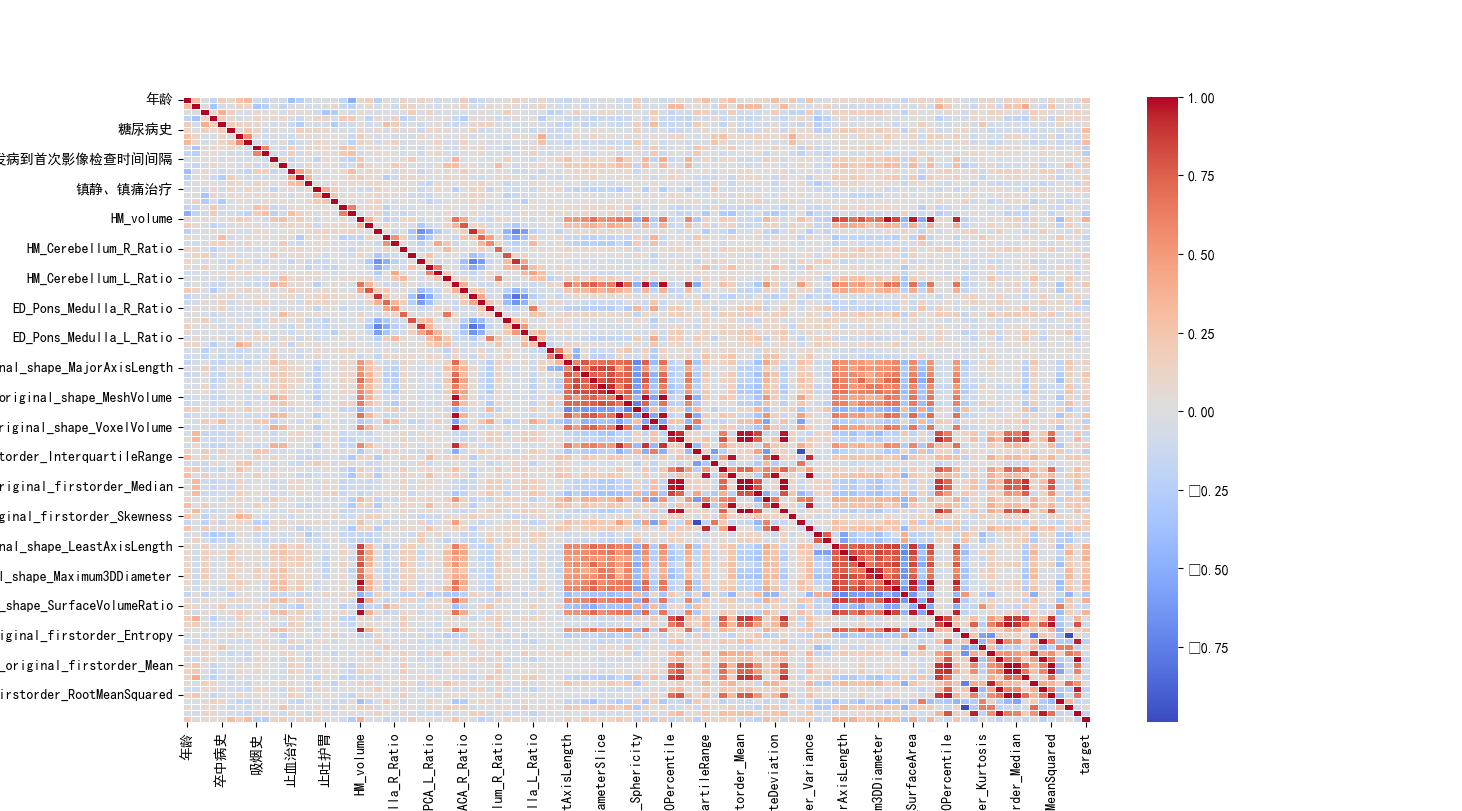
\includegraphics[width=.90\textwidth]{所有列与target之间热力图.png}
				\end{figure}
				
				同样我们还计算了灰色关联系数、斯皮尔曼相关系数以及肯德尔相关系数,计算结果将加入附件中统一上交,这里不在做赘述。此外,我们还计算了多因素对mRS影响的重要性排序,他们从高到底排列展示如图所示:
				
				\begin{figure}[H]
					\centering
					\caption{多因素对mRS影响重要性排序}
					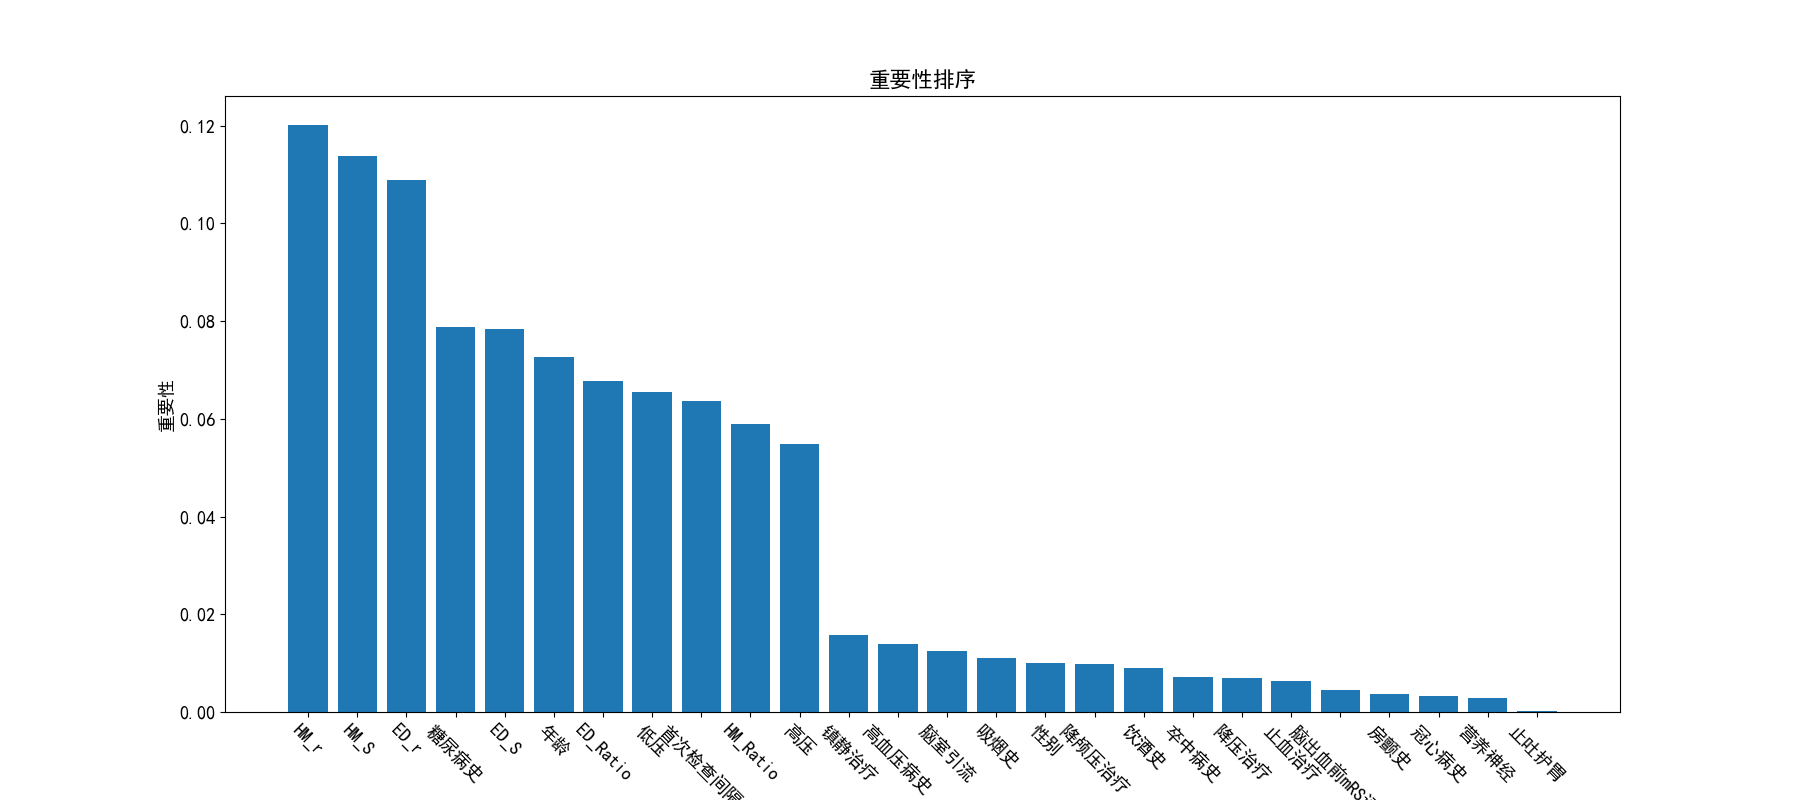
\includegraphics[width=.90\textwidth]{重要性排序.png}
				\end{figure}
				
				通过对上述多个结果的总结分析,我们得出以下结论,并提出以下建议:
				
				\begin{table}[H]
					\centering
					\rowcolors{1}{blue!8}{white}
					\begin{tabularx}{\textwidth}{|X|}
						\hline
						\begin{enumerate}
							\item 血肿体积和形状:血肿的大小和形状对脑出血后的预后影响最大。因此,在治疗过程中应尽快评估和监测血肿的体积和形状,并根据情况采取相应的处理措施。
							
							\item 水肿的体积和形状:水肿是脑出血后常见的并发症之一,对预后产生一定的影响。因此,需要密切关注患者的水肿情况,并及时采取必要的措施进行控制和处理。
							
							\item 糖尿病史:糖尿病与脑出血的预后有一定的关联。对于已知或疑似患有糖尿病的患者,需要加强糖尿病的管理和控制,以减少对预后的不良影响。
							
							\item 年龄和高血压病史:年龄和高血压病史是脑出血的危险因素,也与预后相关。对于年龄较大或有高血压病史的患者,需要更加重视预后评估和治疗,并根据具体情况进行个体化的管理。
							
						\end{enumerate}\\
						\hline
					\end{tabularx}
				\end{table}
				
				
	\section{模型的评价}
		\subsection{模型的优点}
			本次解决赛题过程中使用到了非常多的模型,是我们充分考虑赛题数据量以及问题域从大量模型中筛选出来的,并且我们这次在解决问题一时使用了一个创新性的Channel Attention注意力机制集成学习模型,通过自动学习权重,不断优化权重参数,为模型集成最后的结果提供了排除人因因素的神经网络方法,解放了我们的工作量,我们还在解决问题三的预测问题时,通过投票法整合多个模型之间的预测结果,投票的方式使得单个模型的缺陷或错误会稀释在多模型的投票中,使得模型表达能力更强,具有更好的泛化能力与更强的健壮性。
		\subsection{模型的缺点}
			本次数据集样本数量较少,许多模型在训练过程中存在过拟合的问题,我们在模型建立中加入了很多对模型特征的抽象概括,这使得数据量进一步下降,这将影响到模型训练中的参数优化,更会导致最终的预测结果一定程度上降低,后续应该优先考虑扩张数据的样本量,同时优化我们抽象特征的算法,使得模型能够训练出更好的结果。
	
	
	\begin{thebibliography}{9}%宽度9
	 \bibitem{ma2021temporal} Ma Q , Li R , Wang L ,et al.Temporal trend and attributable risk factors of stroke burden in China, 1990–2019: an analysis for the Global Burden of Disease Study 2019[J].The Lancet Public Health, 2021, 6(12):e897-e906.DOI:10.1016/S2468-2667(21)00228-0.
	 \bibitem{feigin2014global}Feigin V L , Forouzanfar M H , Krishnamurthi R ,et al.Global and regional burden of stroke during 1990-2010: findings from the Global Burden of Disease Study 2010.[J].Lancet, 2014, 383(9913):245-255.DOI:10.1016/S0140-6736(13)61953-4.
	 \bibitem{strock2019bib}朱遂强,刘鸣,等.中国脑出血诊治指南(2019)[J].中华神经科杂志, 2019, 52(12):12.DOI:10.3760/cma.j.issn.1006-7876.2019.12.003.
	 \bibitem{temp1}Chen T , Guestrin C .XGBoost: A Scalable Tree Boosting System[C]//Knowledge Discovery and Data Mining.ACM, 2016.DOI:10.1145/2939672.2939785.
	 \bibitem{temp2}Wang D , Zhang Y , Zhao Y .LightGBM: An Effective miRNA Classification Method in Breast Cancer Patients[C]//Proceedings of the 2017 International Conference on Computational Biology and Bioinformatics.ACM, 2017.DOI:10.1145/3155077.3155079.
	 \bibitem{temp3}Breiman L .Random forest[J].Machine Learning, 2001, 45:5-32.
	\end{thebibliography}
	%\bibliographystyle{gmcm}
	%\bibliography{reference}
	
	
	\clearpage


\end{document}
